\documentclass[review,authoryear]{elsarticle}

\usepackage[utf8]{inputenc}
\usepackage{graphicx}
\usepackage{booktabs}
\usepackage{amsmath}
\usepackage{hyperref}
\usepackage{xcolor}
\usepackage[margin=2.5cm]{geometry}
\usepackage{siunitx}
\sisetup{group-separator={,}, group-minimum-digits=4}

% Auto-generated by generate_macros.py — do not edit by hand.
% Re-run: cd paper_research/code && python generate_macros.py

% ────────────────────────────────────────────────────────────
% Global counts
% ────────────────────────────────────────────────────────────
\newcommand{\nCities}{626}
\newcommand{\nCountries}{28}
\newcommand{\nTotalM}{12.3}
\newcommand{\nClassifiedM}{11.0}
\newcommand{\pctClassified}{89.3}
\newcommand{\pctExcluded}{10.7}
\newcommand{\nMLRestrictedCities}{268}

% ────────────────────────────────────────────────────────────
% Plate 1 — Octant counts and shares
% ────────────────────────────────────────────────────────────
\newcommand{\octHHHcountM}{0.2}
\newcommand{\octHHHpct}{2.2}
\newcommand{\octHHLcountM}{0.4}
\newcommand{\octHHLpct}{4.1}
\newcommand{\octHLHcountM}{0.5}
\newcommand{\octHLHpct}{4.3}
\newcommand{\octHLLcountM}{0.9}
\newcommand{\octHLLpct}{7.9}
\newcommand{\octLHHcountM}{0.4}
\newcommand{\octLHHpct}{3.3}
\newcommand{\octLHLcountM}{0.8}
\newcommand{\octLHLpct}{7.7}
\newcommand{\octLLHcountM}{2.8}
\newcommand{\octLLHpct}{25.4}
\newcommand{\octLLLcountM}{4.9}
\newcommand{\octLLLpct}{45.0}
\newcommand{\octIntensePct}{18.6}
\newcommand{\pctLightTypes}{81}
\newcommand{\pctIntenseAttached}{6}

% ────────────────────────────────────────────────────────────
% Plate 1 — Octant median metric values (Table 1)
% ────────────────────────────────────────────────────────────
\newcommand{\octHHHfsi}{1.81}
\newcommand{\octHHHcont}{0.913}
\newcommand{\octHHHmad}{6.64}
\newcommand{\octHHHretail}{64}
\newcommand{\octHHLfsi}{1.72}
\newcommand{\octHHLcont}{0.902}
\newcommand{\octHHLmad}{1.23}
\newcommand{\octHHLretail}{79}
\newcommand{\octHLHfsi}{1.52}
\newcommand{\octHLHcont}{0.129}
\newcommand{\octHLHmad}{6.86}
\newcommand{\octHLHretail}{98}
\newcommand{\octHLLfsi}{1.47}
\newcommand{\octHLLcont}{0.117}
\newcommand{\octHLLmad}{1.10}
\newcommand{\octHLLretail}{111}
\newcommand{\octLHHfsi}{0.45}
\newcommand{\octLHHcont}{0.872}
\newcommand{\octLHHmad}{6.66}
\newcommand{\octLHHretail}{174}
\newcommand{\octLHLfsi}{0.45}
\newcommand{\octLHLcont}{0.872}
\newcommand{\octLHLmad}{1.00}
\newcommand{\octLHLretail}{189}
\newcommand{\octLLHfsi}{0.30}
\newcommand{\octLLHcont}{0.188}
\newcommand{\octLLHmad}{6.79}
\newcommand{\octLLHretail}{252}
\newcommand{\octLLLfsi}{0.33}
\newcommand{\octLLLcont}{0.221}
\newcommand{\octLLLmad}{1.27}
\newcommand{\octLLLretail}{240}

% ────────────────────────────────────────────────────────────
% Plate 1 — Axis correlations and independence
% ────────────────────────────────────────────────────────────
\newcommand{\nAxesM}{11.0}
\newcommand{\rIntCont}{0.18}
\newcommand{\rIntIrreg}{-0.01}
\newcommand{\rContIrreg}{-0.05}
\newcommand{\rFrontageFSIcity}{0.34}
\newcommand{\maxVIF}{1.0}
\newcommand{\obsExpMin}{0.67}
\newcommand{\obsExpMax}{1.97}
\newcommand{\cramersV}{0.21}

% ────────────────────────────────────────────────────────────
% Plate 1 — Discrimination (eta-squared)
% ────────────────────────────────────────────────────────────
\newcommand{\etaSqGsi}{0.41}
\newcommand{\etaSqHeight}{0.35}
\newcommand{\etaSqMeanFloors}{0.43}
\newcommand{\etaSqBldgDensity}{0.03}
\newcommand{\etaSqCandFsi}{0.58}
\newcommand{\etaSqCandHeight}{0.35}
\newcommand{\etaSqCandHeightVar}{0.15}
\newcommand{\etaSqCandGsiCand}{0.41}
\newcommand{\maxRIntensityCandidates}{0.69}
\newcommand{\pcaTopThree}{49}
\newcommand{\nMorphVars}{20}

% ────────────────────────────────────────────────────────────
% Plate 1 — Missing data rates
% ────────────────────────────────────────────────────────────
\newcommand{\pctMissingFSIfourHundred}{19}
\newcommand{\pctNaNFSIfourHundred}{11}

% ────────────────────────────────────────────────────────────
% Plate 2/3 — City-level axis values
% ────────────────────────────────────────────────────────────
\newcommand{\fsiBarcelona}{1.12}
\newcommand{\fsiAthens}{1.23}
\newcommand{\fsiMadrid}{1.08}
\newcommand{\fsiOslo}{0.26}
\newcommand{\madOslo}{4.8}
\newcommand{\fsiBergen}{0.37}
\newcommand{\madBergen}{6.0}
\newcommand{\fsiHelsinki}{0.35}
\newcommand{\madHelsinki}{3.0}
\newcommand{\fsiStockholm}{0.34}
\newcommand{\madStockholm}{4.2}
\newcommand{\madLiege}{4.7}
\newcommand{\madBrussels}{4.3}
\newcommand{\contNLmed}{0.42}
\newcommand{\contBEmed}{0.39}
\newcommand{\madNLmin}{0.1}
\newcommand{\madNLmax}{4.3}
\newcommand{\madNLmed}{0.8}
\newcommand{\madBEmin}{2.4}
\newcommand{\madBEmax}{6.0}
\newcommand{\madBEmed}{3.9}
\newcommand{\fsiCtryES}{0.79}
\newcommand{\contCtryES}{0.31}
\newcommand{\madCtryES}{2.5}
\newcommand{\fsiCtryBG}{0.70}
\newcommand{\contCtryBG}{0.33}
\newcommand{\madCtryBG}{2.6}
\newcommand{\fsiCtrySK}{0.60}
\newcommand{\contCtrySK}{0.17}
\newcommand{\madCtrySK}{1.6}
\newcommand{\fsiCtryPT}{0.56}
\newcommand{\contCtryPT}{0.37}
\newcommand{\madCtryPT}{4.4}
\newcommand{\fsiCtryAT}{0.53}
\newcommand{\contCtryAT}{0.37}
\newcommand{\madCtryAT}{3.2}
\newcommand{\fsiCtryIT}{0.53}
\newcommand{\contCtryIT}{0.35}
\newcommand{\madCtryIT}{2.7}
\newcommand{\fsiCtryEL}{0.45}
\newcommand{\contCtryEL}{0.49}
\newcommand{\madCtryEL}{3.4}
\newcommand{\fsiCtryLV}{0.56}
\newcommand{\contCtryLV}{0.14}
\newcommand{\madCtryLV}{2.1}
\newcommand{\fsiCtryEE}{0.48}
\newcommand{\contCtryEE}{0.12}
\newcommand{\madCtryEE}{1.7}
\newcommand{\fsiCtryFR}{0.28}
\newcommand{\contCtryFR}{0.31}
\newcommand{\madCtryFR}{3.2}
\newcommand{\fsiCtryIE}{0.35}
\newcommand{\contCtryIE}{0.33}
\newcommand{\madCtryIE}{3.3}
\newcommand{\fsiCtryDE}{0.38}
\newcommand{\contCtryDE}{0.37}
\newcommand{\madCtryDE}{2.8}
\newcommand{\fsiCtryNO}{0.27}
\newcommand{\contCtryNO}{0.28}
\newcommand{\madCtryNO}{4.7}
\newcommand{\fsiCtryCH}{0.35}
\newcommand{\contCtryCH}{0.37}
\newcommand{\madCtryCH}{4.1}
\newcommand{\fsiCtryHR}{0.36}
\newcommand{\contCtryHR}{0.29}
\newcommand{\madCtryHR}{2.9}
\newcommand{\pctContBarcelona}{27}
\newcommand{\pctContAthens}{33}
\newcommand{\pctContMadrid}{21}
\newcommand{\pctContAmsterdam}{22}
\newcommand{\pctContBrussels}{23}
\newcommand{\cvNLcont}{0.18}
\newcommand{\madPolandAvg}{1.9}
\newcommand{\distTreesCoolMed}{34}
\newcommand{\distTreesWarmMed}{101}
\newcommand{\distEatDrinkSouthMed}{187}
\newcommand{\distEatDrinkNorthMed}{383}

% ────────────────────────────────────────────────────────────
% Plate 4 — Building morphometrics by octant
% ────────────────────────────────────────────────────────────
\newcommand{\octHHHfsiFull}{1.81}
\newcommand{\octHHHcontFull}{0.91}
\newcommand{\octHHHheight}{11.2}
\newcommand{\octHHHarea}{161}
\newcommand{\octHHHperim}{56}
\newcommand{\octHHHcorners}{6}
\newcommand{\octHHHcompact}{0.49}
\newcommand{\octHHHvolume}{1849}
\newcommand{\octHHHgsi}{0.55}
\newcommand{\octHHHosr}{0.24}
\newcommand{\octHHHfloors}{3.7}
\newcommand{\octHHHblkPerim}{332}
\newcommand{\octHHHbldgCount}{346}
\newcommand{\octHHHblkCount}{20}
\newcommand{\octHHLfsiFull}{1.72}
\newcommand{\octHHLcontFull}{0.90}
\newcommand{\octHHLheight}{11.7}
\newcommand{\octHHLarea}{190}
\newcommand{\octHHLperim}{61}
\newcommand{\octHHLcorners}{5}
\newcommand{\octHHLcompact}{0.50}
\newcommand{\octHHLvolume}{2388}
\newcommand{\octHHLgsi}{0.51}
\newcommand{\octHHLosr}{0.27}
\newcommand{\octHHLfloors}{3.9}
\newcommand{\octHHLblkPerim}{351}
\newcommand{\octHHLbldgCount}{248}
\newcommand{\octHHLblkCount}{18}
\newcommand{\octHLHfsiFull}{1.52}
\newcommand{\octHLHcontFull}{0.13}
\newcommand{\octHLHheight}{11.3}
\newcommand{\octHLHarea}{178}
\newcommand{\octHLHperim}{59}
\newcommand{\octHLHcorners}{5}
\newcommand{\octHLHcompact}{0.50}
\newcommand{\octHLHvolume}{2130}
\newcommand{\octHLHgsi}{0.42}
\newcommand{\octHLHosr}{0.37}
\newcommand{\octHLHfloors}{4.0}
\newcommand{\octHLHblkPerim}{391}
\newcommand{\octHLHbldgCount}{195}
\newcommand{\octHLHblkCount}{13}
\newcommand{\octHLLfsiFull}{1.47}
\newcommand{\octHLLcontFull}{0.12}
\newcommand{\octHLLheight}{11.9}
\newcommand{\octHLLarea}{217}
\newcommand{\octHLLperim}{65}
\newcommand{\octHLLcorners}{4}
\newcommand{\octHLLcompact}{0.50}
\newcommand{\octHLLvolume}{2850}
\newcommand{\octHLLgsi}{0.39}
\newcommand{\octHLLosr}{0.40}
\newcommand{\octHLLfloors}{4.2}
\newcommand{\octHLLblkPerim}{426}
\newcommand{\octHLLbldgCount}{133}
\newcommand{\octHLLblkCount}{11}
\newcommand{\octLHHfsiFull}{0.45}
\newcommand{\octLHHcontFull}{0.87}
\newcommand{\octLHHheight}{6.0}
\newcommand{\octLHHarea}{96}
\newcommand{\octLHHperim}{42}
\newcommand{\octLHHcorners}{4}
\newcommand{\octLHHcompact}{0.53}
\newcommand{\octLHHvolume}{556}
\newcommand{\octLHHgsi}{0.27}
\newcommand{\octLHHosr}{1.48}
\newcommand{\octLHHfloors}{1.6}
\newcommand{\octLHHblkPerim}{471}
\newcommand{\octLHHbldgCount}{261}
\newcommand{\octLHHblkCount}{9}
\newcommand{\octLHLfsiFull}{0.45}
\newcommand{\octLHLcontFull}{0.87}
\newcommand{\octLHLheight}{6.0}
\newcommand{\octLHLarea}{103}
\newcommand{\octLHLperim}{44}
\newcommand{\octLHLcorners}{4}
\newcommand{\octLHLcompact}{0.52}
\newcommand{\octLHLvolume}{604}
\newcommand{\octLHLgsi}{0.27}
\newcommand{\octLHLosr}{1.47}
\newcommand{\octLHLfloors}{1.6}
\newcommand{\octLHLblkPerim}{509}
\newcommand{\octLHLbldgCount}{216}
\newcommand{\octLHLblkCount}{8}
\newcommand{\octLLHfsiFull}{0.30}
\newcommand{\octLLHcontFull}{0.19}
\newcommand{\octLLHheight}{5.5}
\newcommand{\octLLHarea}{93}
\newcommand{\octLLHperim}{41}
\newcommand{\octLLHcorners}{4}
\newcommand{\octLLHcompact}{0.54}
\newcommand{\octLLHvolume}{527}
\newcommand{\octLLHgsi}{0.21}
\newcommand{\octLLHosr}{2.30}
\newcommand{\octLLHfloors}{1.4}
\newcommand{\octLLHblkPerim}{490}
\newcommand{\octLLHbldgCount}{172}
\newcommand{\octLLHblkCount}{7}
\newcommand{\octLLLfsiFull}{0.33}
\newcommand{\octLLLcontFull}{0.22}
\newcommand{\octLLLheight}{5.7}
\newcommand{\octLLLarea}{97}
\newcommand{\octLLLperim}{42}
\newcommand{\octLLLcorners}{4}
\newcommand{\octLLLcompact}{0.54}
\newcommand{\octLLLvolume}{559}
\newcommand{\octLLLgsi}{0.22}
\newcommand{\octLLLosr}{2.01}
\newcommand{\octLLLfloors}{1.4}
\newcommand{\octLLLblkPerim}{518}
\newcommand{\octLLLbldgCount}{156}
\newcommand{\octLLLblkCount}{6}
\newcommand{\businessSpan}{114}
\newcommand{\octHHHreach}{137}
\newcommand{\octHHLreach}{126}
\newcommand{\octHLHreach}{123}
\newcommand{\octHLLreach}{120}
\newcommand{\octLHHreach}{94}
\newcommand{\octLHLreach}{100}
\newcommand{\octLLHreach}{72}
\newcommand{\octLLLreach}{78}

% ────────────────────────────────────────────────────────────
% Plate 5 — Service distances
% ────────────────────────────────────────────────────────────
\newcommand{\svcTreesMed}{44}
\newcommand{\svcTreesHHH}{97}
\newcommand{\svcTreesHHL}{97}
\newcommand{\svcTreesHLH}{55}
\newcommand{\svcTreesHLL}{58}
\newcommand{\svcTreesLHH}{47}
\newcommand{\svcTreesLHL}{56}
\newcommand{\svcTreesLLH}{33}
\newcommand{\svcTreesLLL}{41}
\newcommand{\svcGreenMed}{129}
\newcommand{\svcGreenHHH}{218}
\newcommand{\svcGreenHHL}{213}
\newcommand{\svcGreenHLH}{156}
\newcommand{\svcGreenHLL}{160}
\newcommand{\svcGreenLHH}{161}
\newcommand{\svcGreenLHL}{168}
\newcommand{\svcGreenLLH}{95}
\newcommand{\svcGreenLLL}{117}
\newcommand{\svcRetailMed}{200}
\newcommand{\svcRetailHHH}{64}
\newcommand{\svcRetailHHL}{79}
\newcommand{\svcRetailHLH}{98}
\newcommand{\svcRetailHLL}{111}
\newcommand{\svcRetailLHH}{174}
\newcommand{\svcRetailLHL}{189}
\newcommand{\svcRetailLLH}{252}
\newcommand{\svcRetailLLL}{240}
\newcommand{\svcBusinessMed}{122}
\newcommand{\svcBusinessHHH}{40}
\newcommand{\svcBusinessHHL}{47}
\newcommand{\svcBusinessHLH}{65}
\newcommand{\svcBusinessHLL}{73}
\newcommand{\svcBusinessLHH}{107}
\newcommand{\svcBusinessLHL}{113}
\newcommand{\svcBusinessLLH}{154}
\newcommand{\svcBusinessLLL}{144}
\newcommand{\svcEatDrinkMed}{279}
\newcommand{\svcEatdrinkHHH}{74}
\newcommand{\svcEatdrinkHHL}{98}
\newcommand{\svcEatdrinkHLH}{112}
\newcommand{\svcEatdrinkHLL}{135}
\newcommand{\svcEatdrinkLHH}{238}
\newcommand{\svcEatdrinkLHL}{278}
\newcommand{\svcEatdrinkLLH}{338}
\newcommand{\svcEatdrinkLLL}{347}
\newcommand{\svcHealthMed}{301}
\newcommand{\svcHealthHHH}{119}
\newcommand{\svcHealthHHL}{133}
\newcommand{\svcHealthHLH}{150}
\newcommand{\svcHealthHLL}{170}
\newcommand{\svcHealthLHH}{267}
\newcommand{\svcHealthLHL}{285}
\newcommand{\svcHealthLLH}{371}
\newcommand{\svcHealthLLL}{358}
\newcommand{\svcEducationMed}{310}
\newcommand{\svcEducationHHH}{136}
\newcommand{\svcEducationHHL}{151}
\newcommand{\svcEducationHLH}{168}
\newcommand{\svcEducationHLL}{185}
\newcommand{\svcEducationLHH}{282}
\newcommand{\svcEducationLHL}{295}
\newcommand{\svcEducationLLH}{379}
\newcommand{\svcEducationLLL}{367}
\newcommand{\svcTransportMed}{237}
\newcommand{\svcTransportHHH}{175}
\newcommand{\svcTransportHHL}{185}
\newcommand{\svcTransportHLH}{160}
\newcommand{\svcTransportHLL}{185}
\newcommand{\svcTransportLHH}{216}
\newcommand{\svcTransportLHL}{252}
\newcommand{\svcTransportLLH}{239}
\newcommand{\svcTransportLLL}{267}
\newcommand{\svcAccommodationMed}{564}
\newcommand{\svcAccommodationHHH}{202}
\newcommand{\svcAccommodationHHL}{270}
\newcommand{\svcAccommodationHLH}{279}
\newcommand{\svcAccommodationHLL}{346}
\newcommand{\svcAccommodationLHH}{529}
\newcommand{\svcAccommodationLHL}{595}
\newcommand{\svcAccommodationLLH}{630}
\newcommand{\svcAccommodationLLL}{662}
\newcommand{\svcArtsMed}{491}
\newcommand{\svcArtsHHH}{183}
\newcommand{\svcArtsHHL}{221}
\newcommand{\svcArtsHLH}{241}
\newcommand{\svcArtsHLL}{281}
\newcommand{\svcArtsLHH}{462}
\newcommand{\svcArtsLHL}{499}
\newcommand{\svcArtsLLH}{579}
\newcommand{\svcArtsLLL}{580}
\newcommand{\svcAttractionsMed}{445}
\newcommand{\svcAttractionsHHH}{166}
\newcommand{\svcAttractionsHHL}{214}
\newcommand{\svcAttractionsHLH}{216}
\newcommand{\svcAttractionsHLL}{260}
\newcommand{\svcAttractionsLHH}{422}
\newcommand{\svcAttractionsLHL}{458}
\newcommand{\svcAttractionsLLH}{514}
\newcommand{\svcAttractionsLLL}{528}
\newcommand{\svcReligiousMed}{577}
\newcommand{\svcReligiousHHH}{234}
\newcommand{\svcReligiousHHL}{297}
\newcommand{\svcReligiousHLH}{327}
\newcommand{\svcReligiousHLL}{396}
\newcommand{\svcReligiousLHH}{511}
\newcommand{\svcReligiousLHL}{576}
\newcommand{\svcReligiousLLH}{654}
\newcommand{\svcReligiousLLL}{677}
\newcommand{\retailFoldHHHtoLLL}{3.8}
\newcommand{\eatDrinkFoldHHHtoLLL}{4.7}
\newcommand{\transportFoldHHHtoLLL}{1.5}
\newcommand{\eatDrinkOslo}{415}
\newcommand{\eatDrinkBergen}{396}
\newcommand{\eatDrinkBarcelona}{136}
\newcommand{\eatDrinkAthens}{169}

% ────────────────────────────────────────────────────────────
% Plate 8 — Demographics by octant
% ────────────────────────────────────────────────────────────
\newcommand{\octHHHpopDens}{9964}
\newcommand{\octHHHyouth}{12}
\newcommand{\octHHHelderly}{20}
\newcommand{\octHHLpopDens}{10423}
\newcommand{\octHHLyouth}{13}
\newcommand{\octHHLelderly}{20}
\newcommand{\octHLHpopDens}{8469}
\newcommand{\octHLHyouth}{13}
\newcommand{\octHLHelderly}{20}
\newcommand{\octHLLpopDens}{8366}
\newcommand{\octHLLyouth}{13}
\newcommand{\octHLLelderly}{20}
\newcommand{\octLHHpopDens}{4078}
\newcommand{\octLHHyouth}{15}
\newcommand{\octLHHelderly}{20}
\newcommand{\octLHLpopDens}{4174}
\newcommand{\octLHLyouth}{15}
\newcommand{\octLHLelderly}{19}
\newcommand{\octLLHpopDens}{2953}
\newcommand{\octLLHyouth}{15}
\newcommand{\octLLHelderly}{20}
\newcommand{\octLLLpopDens}{3187}
\newcommand{\octLLLyouth}{15}
\newcommand{\octLLLelderly}{20}
\newcommand{\octHHHemploy}{42}
\newcommand{\octHHHworkAge}{67}
\newcommand{\octHHLemploy}{43}
\newcommand{\octHHLworkAge}{67}
\newcommand{\octHLHemploy}{43}
\newcommand{\octHLHworkAge}{66}
\newcommand{\octHLLemploy}{45}
\newcommand{\octHLLworkAge}{66}
\newcommand{\octLHHemploy}{45}
\newcommand{\octLHHworkAge}{65}
\newcommand{\octLHLemploy}{47}
\newcommand{\octLHLworkAge}{65}
\newcommand{\octLLHemploy}{46}
\newcommand{\octLLHworkAge}{64}
\newcommand{\octLLLemploy}{47}
\newcommand{\octLLLworkAge}{65}
\newcommand{\youthIntense}{13}
\newcommand{\youthLight}{15}
\newcommand{\elderlyMin}{19}
\newcommand{\elderlyMax}{20}
\newcommand{\workAgeIntenseMin}{66}
\newcommand{\workAgeIntenseMax}{67}
\newcommand{\workAgeLightMin}{64}
\newcommand{\workAgeLightMax}{65}
\newcommand{\employIntenseMin}{42}
\newcommand{\employIntenseMax}{45}
\newcommand{\employLightMin}{45}
\newcommand{\employLightMax}{47}
\newcommand{\popDensIntenseMin}{8366}
\newcommand{\popDensLightMax}{4174}

% ────────────────────────────────────────────────────────────
% Appendix — within-city demographic robustness
% ────────────────────────────────────────────────────────────
\newcommand{\demoChildGap}{+2.0}
\newcommand{\demoChildDelta}{+0.32}
\newcommand{\demoChildPct}{86}
\newcommand{\demoWorkGap}{-1.8}
\newcommand{\demoWorkDelta}{-0.24}
\newcommand{\demoWorkPct}{63}
\newcommand{\demoElderGap}{+0.1}
\newcommand{\demoElderDelta}{+0.06}
\newcommand{\demoElderPct}{50}
\newcommand{\demoEmpGap}{+2.9}
\newcommand{\demoEmpDelta}{-0.04}
\newcommand{\demoEmpPct}{53}

% ────────────────────────────────────────────────────────────
% Plate 9 — Green vs retail correlation
% ────────────────────────────────────────────────────────────
\newcommand{\rGreenRetail}{-0.08}
\newcommand{\pGreenRetail}{0.05}
\newcommand{\rhoGreenRetail}{-0.04}
\newcommand{\pRhoGreenRetail}{0.39}
\newcommand{\nGreenRetail}{602}
\newcommand{\leverageGreenRetailCity}{Maasvlakte}
\newcommand{\leverageGreenRetailDelta}{0.039}
\newcommand{\leverageGreenRetailRwithout}{-0.12}

% ────────────────────────────────────────────────────────────
% Plate 10 — Paired comparisons
% ────────────────────────────────────────────────────────────
\newcommand{\compNordicFSI}{0.35}
\newcommand{\compMedFSI}{1.08}
\newcommand{\compNordicHeight}{6.2}
\newcommand{\compMedHeight}{8.5}
\newcommand{\compNordicGSI}{0.20}
\newcommand{\compMedGSI}{0.41}
\newcommand{\compNordicCont}{0.26}
\newcommand{\compMedCont}{0.44}
\newcommand{\compNordicMAD}{4.2}
\newcommand{\compMedMAD}{2.5}
\newcommand{\compNordicStreetDens}{349}
\newcommand{\compMedStreetDens}{399}
\newcommand{\compNordicRetail}{258}
\newcommand{\compMedRetail}{122}
\newcommand{\compNordicEatDrink}{365}
\newcommand{\compMedEatDrink}{169}
\newcommand{\compNordicTrees}{30}
\newcommand{\compMedTrees}{105}
\newcommand{\compNordicGreen}{112}
\newcommand{\compMedGreen}{174}
\newcommand{\compNLFSI}{0.49}
\newcommand{\compBEFSI}{0.41}
\newcommand{\compNLHeight}{6.2}
\newcommand{\compBEHeight}{5.9}
\newcommand{\compNLGSI}{0.31}
\newcommand{\compBEGSI}{0.30}
\newcommand{\compNLCont}{0.43}
\newcommand{\compBECont}{0.39}
\newcommand{\compNLMAD}{0.3}
\newcommand{\compBEMAD}{3.9}
\newcommand{\compNLStreetDens}{472}
\newcommand{\compBEStreetDens}{223}
\newcommand{\compNLRetail}{217}
\newcommand{\compBERetail}{205}
\newcommand{\compNLEatDrink}{304}
\newcommand{\compBEEatDrink}{266}
\newcommand{\compNLTrees}{52}
\newcommand{\compBETrees}{46}
\newcommand{\compNLGreen}{126}
\newcommand{\compBEGreen}{173}
\newcommand{\compLCFSI}{0.35}
\newcommand{\compBalticFSI}{0.47}
\newcommand{\compLCHeight}{5.1}
\newcommand{\compBalticHeight}{6.6}
\newcommand{\compLCGSI}{0.28}
\newcommand{\compBalticGSI}{0.20}
\newcommand{\compLCCont}{0.41}
\newcommand{\compBalticCont}{0.17}
\newcommand{\compLCMAD}{1.4}
\newcommand{\compBalticMAD}{1.6}
\newcommand{\compLCStreetDens}{394}
\newcommand{\compBalticStreetDens}{432}
\newcommand{\compLCRetail}{233}
\newcommand{\compBalticRetail}{218}
\newcommand{\compLCEatDrink}{360}
\newcommand{\compBalticEatDrink}{338}
\newcommand{\compLCTrees}{46}
\newcommand{\compBalticTrees}{33}
\newcommand{\compLCGreen}{117}
\newcommand{\compBalticGreen}{123}
\newcommand{\compPLFSI}{0.36}
\newcommand{\compROFSI}{0.39}
\newcommand{\compPLHeight}{5.2}
\newcommand{\compROHeight}{5.0}
\newcommand{\compPLGSI}{0.19}
\newcommand{\compROGSI}{0.26}
\newcommand{\compPLCont}{0.18}
\newcommand{\compROCont}{0.37}
\newcommand{\compPLMAD}{1.9}
\newcommand{\compROMAD}{3.0}
\newcommand{\compPLStreetDens}{460}
\newcommand{\compROStreetDens}{216}
\newcommand{\compPLRetail}{163}
\newcommand{\compRORetail}{169}
\newcommand{\compPLEatDrink}{307}
\newcommand{\compROEatDrink}{250}
\newcommand{\compPLTrees}{42}
\newcommand{\compROTrees}{53}
\newcommand{\compPLGreen}{116}
\newcommand{\compROGreen}{207}

% ────────────────────────────────────────────────────────────
% Plate 11 — Density quintile form gaps
% ────────────────────────────────────────────────────────────
\newcommand{\dqMedianOne}{922}
\newcommand{\dqMedianTwo}{2370}
\newcommand{\dqMedianThree}{3848}
\newcommand{\dqMedianFour}{5864}
\newcommand{\dqMedianFive}{10678}
\newcommand{\dqRetailQOnelo}{145}
\newcommand{\dqRetailQOnehi}{405}
\newcommand{\dqRetailQOnegap}{260}
\newcommand{\dqRetailQOnebest}{HHH}
\newcommand{\dqRetailQOneworst}{LLH}
\newcommand{\dqRetailQTwolo}{98}
\newcommand{\dqRetailQTwohi}{287}
\newcommand{\dqRetailQTwogap}{189}
\newcommand{\dqRetailQTwobest}{HHH}
\newcommand{\dqRetailQTwoworst}{LLH}
\newcommand{\dqRetailQThreelo}{77}
\newcommand{\dqRetailQThreehi}{232}
\newcommand{\dqRetailQThreegap}{155}
\newcommand{\dqRetailQThreebest}{HHH}
\newcommand{\dqRetailQThreeworst}{LLL}
\newcommand{\dqRetailQFourlo}{63}
\newcommand{\dqRetailQFourhi}{188}
\newcommand{\dqRetailQFourgap}{124}
\newcommand{\dqRetailQFourbest}{HHH}
\newcommand{\dqRetailQFourworst}{LLL}
\newcommand{\dqRetailQFivelo}{61}
\newcommand{\dqRetailQFivehi}{152}
\newcommand{\dqRetailQFivegap}{91}
\newcommand{\dqRetailQFivebest}{HHH}
\newcommand{\dqRetailQFiveworst}{LLH}
\newcommand{\dqEducationQOnelo}{340}
\newcommand{\dqEducationQOnehi}{697}
\newcommand{\dqEducationQOnegap}{357}
\newcommand{\dqEducationQOnebest}{HHH}
\newcommand{\dqEducationQOneworst}{LLL}
\newcommand{\dqEducationQTwolo}{210}
\newcommand{\dqEducationQTwohi}{441}
\newcommand{\dqEducationQTwogap}{231}
\newcommand{\dqEducationQTwobest}{HHH}
\newcommand{\dqEducationQTwoworst}{LLL}
\newcommand{\dqEducationQThreelo}{158}
\newcommand{\dqEducationQThreehi}{333}
\newcommand{\dqEducationQThreegap}{175}
\newcommand{\dqEducationQThreebest}{HHH}
\newcommand{\dqEducationQThreeworst}{LLH}
\newcommand{\dqEducationQFourlo}{140}
\newcommand{\dqEducationQFourhi}{268}
\newcommand{\dqEducationQFourgap}{128}
\newcommand{\dqEducationQFourbest}{HHH}
\newcommand{\dqEducationQFourworst}{LLL}
\newcommand{\dqEducationQFivelo}{131}
\newcommand{\dqEducationQFivehi}{225}
\newcommand{\dqEducationQFivegap}{93}
\newcommand{\dqEducationQFivebest}{HHH}
\newcommand{\dqEducationQFiveworst}{LLH}
\newcommand{\dqTransportQOnelo}{227}
\newcommand{\dqTransportQOnehi}{359}
\newcommand{\dqTransportQOnegap}{132}
\newcommand{\dqTransportQOnebest}{HHH}
\newcommand{\dqTransportQOneworst}{LLL}
\newcommand{\dqTransportQTwolo}{187}
\newcommand{\dqTransportQTwohi}{278}
\newcommand{\dqTransportQTwogap}{92}
\newcommand{\dqTransportQTwobest}{HHH}
\newcommand{\dqTransportQTwoworst}{LLL}
\newcommand{\dqTransportQThreelo}{185}
\newcommand{\dqTransportQThreehi}{248}
\newcommand{\dqTransportQThreegap}{63}
\newcommand{\dqTransportQThreebest}{HLH}
\newcommand{\dqTransportQThreeworst}{LLL}
\newcommand{\dqTransportQFourlo}{168}
\newcommand{\dqTransportQFourhi}{240}
\newcommand{\dqTransportQFourgap}{72}
\newcommand{\dqTransportQFourbest}{HLH}
\newcommand{\dqTransportQFourworst}{LHL}
\newcommand{\dqTransportQFivelo}{148}
\newcommand{\dqTransportQFivehi}{228}
\newcommand{\dqTransportQFivegap}{80}
\newcommand{\dqTransportQFivebest}{HLH}
\newcommand{\dqTransportQFiveworst}{LHL}
\newcommand{\dqGreenQOnelo}{41}
\newcommand{\dqGreenQOnehi}{231}
\newcommand{\dqGreenQOnegap}{189}
\newcommand{\dqGreenQOnebest}{LLH}
\newcommand{\dqGreenQOneworst}{HHL}
\newcommand{\dqGreenQTwolo}{88}
\newcommand{\dqGreenQTwohi}{164}
\newcommand{\dqGreenQTwogap}{76}
\newcommand{\dqGreenQTwobest}{HLH}
\newcommand{\dqGreenQTwoworst}{HHL}
\newcommand{\dqGreenQThreelo}{119}
\newcommand{\dqGreenQThreehi}{177}
\newcommand{\dqGreenQThreegap}{58}
\newcommand{\dqGreenQThreebest}{HLH}
\newcommand{\dqGreenQThreeworst}{HHH}
\newcommand{\dqGreenQFourlo}{139}
\newcommand{\dqGreenQFourhi}{203}
\newcommand{\dqGreenQFourgap}{64}
\newcommand{\dqGreenQFourbest}{LLH}
\newcommand{\dqGreenQFourworst}{HHH}
\newcommand{\dqGreenQFivelo}{159}
\newcommand{\dqGreenQFivehi}{232}
\newcommand{\dqGreenQFivegap}{73}
\newcommand{\dqGreenQFivebest}{LLH}
\newcommand{\dqGreenQFiveworst}{HHH}
\newcommand{\retailContMed}{203}
\newcommand{\dqRetailQThreegapPct}{76}

% ────────────────────────────────────────────────────────────
% Plate 6 — Desert fractions (no service within 400m)
% ────────────────────────────────────────────────────────────
\newcommand{\desertTreesHHH}{2}
\newcommand{\desertTreesHHL}{2}
\newcommand{\desertTreesHLH}{1}
\newcommand{\desertTreesHLL}{2}
\newcommand{\desertTreesLHH}{1}
\newcommand{\desertTreesLHL}{2}
\newcommand{\desertTreesLLH}{1}
\newcommand{\desertTreesLLL}{2}
\newcommand{\desertGreenHHH}{17}
\newcommand{\desertGreenHHL}{17}
\newcommand{\desertGreenHLH}{13}
\newcommand{\desertGreenHLL}{14}
\newcommand{\desertGreenLHH}{11}
\newcommand{\desertGreenLHL}{12}
\newcommand{\desertGreenLLH}{7}
\newcommand{\desertGreenLLL}{9}
\newcommand{\desertRetailHHH}{1}
\newcommand{\desertRetailHHL}{2}
\newcommand{\desertRetailHLH}{3}
\newcommand{\desertRetailHLL}{5}
\newcommand{\desertRetailLHH}{14}
\newcommand{\desertRetailLHL}{15}
\newcommand{\desertRetailLLH}{28}
\newcommand{\desertRetailLLL}{26}
\newcommand{\desertBusinessHHH}{0}
\newcommand{\desertBusinessHHL}{1}
\newcommand{\desertBusinessHLH}{1}
\newcommand{\desertBusinessHLL}{1}
\newcommand{\desertBusinessLHH}{3}
\newcommand{\desertBusinessLHL}{4}
\newcommand{\desertBusinessLLH}{12}
\newcommand{\desertBusinessLLL}{10}
\newcommand{\desertEatDrinkHHH}{2}
\newcommand{\desertEatDrinkHHL}{4}
\newcommand{\desertEatDrinkHLH}{6}
\newcommand{\desertEatDrinkHLL}{9}
\newcommand{\desertEatDrinkLHH}{26}
\newcommand{\desertEatDrinkLHL}{32}
\newcommand{\desertEatDrinkLLH}{42}
\newcommand{\desertEatDrinkLLL}{43}
\newcommand{\desertHealthHHH}{5}
\newcommand{\desertHealthHHL}{8}
\newcommand{\desertHealthHLH}{10}
\newcommand{\desertHealthHLL}{15}
\newcommand{\desertHealthLHH}{30}
\newcommand{\desertHealthLHL}{33}
\newcommand{\desertHealthLLH}{46}
\newcommand{\desertHealthLLL}{45}
\newcommand{\desertEducationHHH}{4}
\newcommand{\desertEducationHHL}{7}
\newcommand{\desertEducationHLH}{10}
\newcommand{\desertEducationHLL}{14}
\newcommand{\desertEducationLHH}{31}
\newcommand{\desertEducationLHL}{33}
\newcommand{\desertEducationLLH}{47}
\newcommand{\desertEducationLLL}{46}
\newcommand{\desertTransportHHH}{8}
\newcommand{\desertTransportHHL}{10}
\newcommand{\desertTransportHLH}{9}
\newcommand{\desertTransportHLL}{12}
\newcommand{\desertTransportLHH}{16}
\newcommand{\desertTransportLHL}{22}
\newcommand{\desertTransportLLH}{25}
\newcommand{\desertTransportLLL}{28}
\newcommand{\desertAccommodationHHH}{23}
\newcommand{\desertAccommodationHHL}{34}
\newcommand{\desertAccommodationHLH}{34}
\newcommand{\desertAccommodationHLL}{43}
\newcommand{\desertAccommodationLHH}{63}
\newcommand{\desertAccommodationLHL}{70}
\newcommand{\desertAccommodationLLH}{72}
\newcommand{\desertAccommodationLLL}{75}
\newcommand{\desertArtsHHH}{15}
\newcommand{\desertArtsHHL}{21}
\newcommand{\desertArtsHLH}{25}
\newcommand{\desertArtsHLL}{32}
\newcommand{\desertArtsLHH}{58}
\newcommand{\desertArtsLHL}{62}
\newcommand{\desertArtsLLH}{69}
\newcommand{\desertArtsLLL}{70}
\newcommand{\desertAttractionsHHH}{13}
\newcommand{\desertAttractionsHHL}{20}
\newcommand{\desertAttractionsHLH}{21}
\newcommand{\desertAttractionsHLL}{28}
\newcommand{\desertAttractionsLHH}{53}
\newcommand{\desertAttractionsLHL}{57}
\newcommand{\desertAttractionsLLH}{63}
\newcommand{\desertAttractionsLLL}{65}
\newcommand{\desertReligiousHHH}{22}
\newcommand{\desertReligiousHHL}{33}
\newcommand{\desertReligiousHLH}{38}
\newcommand{\desertReligiousHLL}{49}
\newcommand{\desertReligiousLHH}{63}
\newcommand{\desertReligiousLHL}{70}
\newcommand{\desertReligiousLLH}{75}
\newcommand{\desertReligiousLLL}{77}

% ────────────────────────────────────────────────────────────
% Plate 7 — P25/P75 unevenness
% ────────────────────────────────────────────────────────────
\newcommand{\iqrTreesHHH}{128}
\newcommand{\ptwofiveTreesHHH}{41}
\newcommand{\psevenfiveTreesHHH}{169}
\newcommand{\iqrTreesHHL}{132}
\newcommand{\ptwofiveTreesHHL}{39}
\newcommand{\psevenfiveTreesHHL}{170}
\newcommand{\iqrTreesHLH}{103}
\newcommand{\ptwofiveTreesHLH}{16}
\newcommand{\psevenfiveTreesHLH}{119}
\newcommand{\iqrTreesHLL}{113}
\newcommand{\ptwofiveTreesHLL}{16}
\newcommand{\psevenfiveTreesHLL}{130}
\newcommand{\iqrTreesLHH}{77}
\newcommand{\ptwofiveTreesLHH}{20}
\newcommand{\psevenfiveTreesLHH}{97}
\newcommand{\iqrTreesLHL}{89}
\newcommand{\ptwofiveTreesLHL}{23}
\newcommand{\psevenfiveTreesLHL}{111}
\newcommand{\iqrTreesLLH}{74}
\newcommand{\ptwofiveTreesLLH}{10}
\newcommand{\psevenfiveTreesLLH}{83}
\newcommand{\iqrTreesLLL}{89}
\newcommand{\ptwofiveTreesLLL}{12}
\newcommand{\psevenfiveTreesLLL}{101}
\newcommand{\iqrGreenHHH}{224}
\newcommand{\ptwofiveGreenHHH}{119}
\newcommand{\psevenfiveGreenHHH}{343}
\newcommand{\iqrGreenHHL}{225}
\newcommand{\ptwofiveGreenHHL}{116}
\newcommand{\psevenfiveGreenHHL}{342}
\newcommand{\iqrGreenHLH}{242}
\newcommand{\ptwofiveGreenHLH}{50}
\newcommand{\psevenfiveGreenHLH}{292}
\newcommand{\iqrGreenHLL}{242}
\newcommand{\ptwofiveGreenHLL}{54}
\newcommand{\psevenfiveGreenHLL}{296}
\newcommand{\iqrGreenLHH}{194}
\newcommand{\ptwofiveGreenLHH}{81}
\newcommand{\psevenfiveGreenLHH}{275}
\newcommand{\iqrGreenLHL}{197}
\newcommand{\ptwofiveGreenLHL}{87}
\newcommand{\psevenfiveGreenLHL}{284}
\newcommand{\iqrGreenLLH}{201}
\newcommand{\ptwofiveGreenLLH}{13}
\newcommand{\psevenfiveGreenLLH}{214}
\newcommand{\iqrGreenLLL}{215}
\newcommand{\ptwofiveGreenLLL}{25}
\newcommand{\psevenfiveGreenLLL}{241}
\newcommand{\iqrRetailHHH}{96}
\newcommand{\ptwofiveRetailHHH}{22}
\newcommand{\psevenfiveRetailHHH}{118}
\newcommand{\iqrRetailHHL}{110}
\newcommand{\ptwofiveRetailHHL}{29}
\newcommand{\psevenfiveRetailHHL}{139}
\newcommand{\iqrRetailHLH}{122}
\newcommand{\ptwofiveRetailHLH}{50}
\newcommand{\psevenfiveRetailHLH}{172}
\newcommand{\iqrRetailHLL}{135}
\newcommand{\ptwofiveRetailHLL}{58}
\newcommand{\psevenfiveRetailHLL}{193}
\newcommand{\iqrRetailLHH}{206}
\newcommand{\ptwofiveRetailLHH}{90}
\newcommand{\psevenfiveRetailLHH}{296}
\newcommand{\iqrRetailLHL}{213}
\newcommand{\ptwofiveRetailLHL}{102}
\newcommand{\psevenfiveRetailLHL}{315}
\newcommand{\iqrRetailLLH}{295}
\newcommand{\ptwofiveRetailLLH}{135}
\newcommand{\psevenfiveRetailLLH}{431}
\newcommand{\iqrRetailLLL}{277}
\newcommand{\ptwofiveRetailLLL}{130}
\newcommand{\psevenfiveRetailLLL}{407}
\newcommand{\iqrBusinessHHH}{65}
\newcommand{\ptwofiveBusinessHHH}{16}
\newcommand{\psevenfiveBusinessHHH}{81}
\newcommand{\iqrBusinessHHL}{76}
\newcommand{\ptwofiveBusinessHHL}{18}
\newcommand{\psevenfiveBusinessHHL}{93}
\newcommand{\iqrBusinessHLH}{81}
\newcommand{\ptwofiveBusinessHLH}{33}
\newcommand{\psevenfiveBusinessHLH}{114}
\newcommand{\iqrBusinessHLL}{90}
\newcommand{\ptwofiveBusinessHLL}{37}
\newcommand{\psevenfiveBusinessHLL}{127}
\newcommand{\iqrBusinessLHH}{130}
\newcommand{\ptwofiveBusinessLHH}{51}
\newcommand{\psevenfiveBusinessLHH}{181}
\newcommand{\iqrBusinessLHL}{130}
\newcommand{\ptwofiveBusinessLHL}{57}
\newcommand{\psevenfiveBusinessLHL}{188}
\newcommand{\iqrBusinessLLH}{186}
\newcommand{\ptwofiveBusinessLLH}{82}
\newcommand{\psevenfiveBusinessLLH}{268}
\newcommand{\iqrBusinessLLL}{172}
\newcommand{\ptwofiveBusinessLLL}{77}
\newcommand{\psevenfiveBusinessLLL}{249}
\newcommand{\iqrEatDrinkHHH}{110}
\newcommand{\ptwofiveEatDrinkHHH}{27}
\newcommand{\psevenfiveEatDrinkHHH}{138}
\newcommand{\iqrEatDrinkHHL}{129}
\newcommand{\ptwofiveEatDrinkHHL}{42}
\newcommand{\psevenfiveEatDrinkHHL}{171}
\newcommand{\iqrEatDrinkHLH}{143}
\newcommand{\ptwofiveEatDrinkHLH}{56}
\newcommand{\psevenfiveEatDrinkHLH}{200}
\newcommand{\iqrEatDrinkHLL}{169}
\newcommand{\ptwofiveEatDrinkHLL}{69}
\newcommand{\psevenfiveEatDrinkHLL}{239}
\newcommand{\iqrEatDrinkLHH}{287}
\newcommand{\ptwofiveEatDrinkLHH}{124}
\newcommand{\psevenfiveEatDrinkLHH}{411}
\newcommand{\iqrEatDrinkLHL}{304}
\newcommand{\ptwofiveEatDrinkLHL}{155}
\newcommand{\psevenfiveEatDrinkLHL}{459}
\newcommand{\iqrEatDrinkLLH}{383}
\newcommand{\ptwofiveEatDrinkLLH}{184}
\newcommand{\psevenfiveEatDrinkLLH}{567}
\newcommand{\iqrEatDrinkLLL}{376}
\newcommand{\ptwofiveEatDrinkLLL}{195}
\newcommand{\psevenfiveEatDrinkLLL}{571}
\newcommand{\iqrHealthHHH}{132}
\newcommand{\ptwofiveHealthHHH}{65}
\newcommand{\psevenfiveHealthHHH}{197}
\newcommand{\iqrHealthHHL}{151}
\newcommand{\ptwofiveHealthHHL}{73}
\newcommand{\psevenfiveHealthHHL}{223}
\newcommand{\iqrHealthHLH}{171}
\newcommand{\ptwofiveHealthHLH}{84}
\newcommand{\psevenfiveHealthHLH}{255}
\newcommand{\iqrHealthHLL}{200}
\newcommand{\ptwofiveHealthHLL}{94}
\newcommand{\psevenfiveHealthHLL}{294}
\newcommand{\iqrHealthLHH}{301}
\newcommand{\ptwofiveHealthLHH}{148}
\newcommand{\psevenfiveHealthLHH}{449}
\newcommand{\iqrHealthLHL}{309}
\newcommand{\ptwofiveHealthLHL}{163}
\newcommand{\psevenfiveHealthLHL}{472}
\newcommand{\iqrHealthLLH}{416}
\newcommand{\ptwofiveHealthLLH}{207}
\newcommand{\psevenfiveHealthLLH}{623}
\newcommand{\iqrHealthLLL}{404}
\newcommand{\ptwofiveHealthLLL}{202}
\newcommand{\psevenfiveHealthLLL}{606}
\newcommand{\iqrEducationHHH}{129}
\newcommand{\ptwofiveEducationHHH}{81}
\newcommand{\psevenfiveEducationHHH}{210}
\newcommand{\iqrEducationHHL}{145}
\newcommand{\ptwofiveEducationHHL}{90}
\newcommand{\psevenfiveEducationHHL}{235}
\newcommand{\iqrEducationHLH}{168}
\newcommand{\ptwofiveEducationHLH}{99}
\newcommand{\psevenfiveEducationHLH}{267}
\newcommand{\iqrEducationHLL}{189}
\newcommand{\ptwofiveEducationHLL}{109}
\newcommand{\psevenfiveEducationHLL}{297}
\newcommand{\iqrEducationLHH}{288}
\newcommand{\ptwofiveEducationLHH}{165}
\newcommand{\psevenfiveEducationLHH}{454}
\newcommand{\iqrEducationLHL}{298}
\newcommand{\ptwofiveEducationLHL}{176}
\newcommand{\psevenfiveEducationLHL}{474}
\newcommand{\iqrEducationLLH}{406}
\newcommand{\ptwofiveEducationLLH}{219}
\newcommand{\psevenfiveEducationLLH}{625}
\newcommand{\iqrEducationLLL}{400}
\newcommand{\ptwofiveEducationLLL}{212}
\newcommand{\psevenfiveEducationLLL}{612}
\newcommand{\iqrTransportHHH}{153}
\newcommand{\ptwofiveTransportHHH}{109}
\newcommand{\psevenfiveTransportHHH}{262}
\newcommand{\iqrTransportHHL}{159}
\newcommand{\ptwofiveTransportHHL}{118}
\newcommand{\psevenfiveTransportHHL}{277}
\newcommand{\iqrTransportHLH}{170}
\newcommand{\ptwofiveTransportHLH}{89}
\newcommand{\psevenfiveTransportHLH}{259}
\newcommand{\iqrTransportHLL}{188}
\newcommand{\ptwofiveTransportHLL}{105}
\newcommand{\psevenfiveTransportHLL}{293}
\newcommand{\iqrTransportLHH}{202}
\newcommand{\ptwofiveTransportLHH}{130}
\newcommand{\psevenfiveTransportLHH}{332}
\newcommand{\iqrTransportLHL}{218}
\newcommand{\ptwofiveTransportLHL}{159}
\newcommand{\psevenfiveTransportLHL}{378}
\newcommand{\iqrTransportLLH}{268}
\newcommand{\ptwofiveTransportLLH}{131}
\newcommand{\psevenfiveTransportLLH}{399}
\newcommand{\iqrTransportLLL}{276}
\newcommand{\ptwofiveTransportLLL}{154}
\newcommand{\psevenfiveTransportLLL}{430}
\newcommand{\iqrAccommodationHHH}{283}
\newcommand{\ptwofiveAccommodationHHH}{98}
\newcommand{\psevenfiveAccommodationHHH}{381}
\newcommand{\iqrAccommodationHHL}{362}
\newcommand{\ptwofiveAccommodationHHL}{137}
\newcommand{\psevenfiveAccommodationHHL}{499}
\newcommand{\iqrAccommodationHLH}{346}
\newcommand{\ptwofiveAccommodationHLH}{148}
\newcommand{\psevenfiveAccommodationHLH}{494}
\newcommand{\iqrAccommodationHLL}{426}
\newcommand{\ptwofiveAccommodationHLL}{184}
\newcommand{\psevenfiveAccommodationHLL}{610}
\newcommand{\iqrAccommodationLHH}{554}
\newcommand{\ptwofiveAccommodationLHH}{297}
\newcommand{\psevenfiveAccommodationLHH}{850}
\newcommand{\iqrAccommodationLHL}{566}
\newcommand{\ptwofiveAccommodationLHL}{349}
\newcommand{\psevenfiveAccommodationLHL}{915}
\newcommand{\iqrAccommodationLLH}{593}
\newcommand{\ptwofiveAccommodationLLH}{370}
\newcommand{\psevenfiveAccommodationLLH}{963}
\newcommand{\iqrAccommodationLLL}{599}
\newcommand{\ptwofiveAccommodationLLL}{396}
\newcommand{\psevenfiveAccommodationLLL}{995}
\newcommand{\iqrArtsHHH}{200}
\newcommand{\ptwofiveArtsHHH}{105}
\newcommand{\psevenfiveArtsHHH}{305}
\newcommand{\iqrArtsHHL}{235}
\newcommand{\ptwofiveArtsHHL}{128}
\newcommand{\psevenfiveArtsHHL}{364}
\newcommand{\iqrArtsHLH}{263}
\newcommand{\ptwofiveArtsHLH}{137}
\newcommand{\psevenfiveArtsHLH}{400}
\newcommand{\iqrArtsHLL}{302}
\newcommand{\ptwofiveArtsHLL}{161}
\newcommand{\psevenfiveArtsHLL}{463}
\newcommand{\iqrArtsLHH}{458}
\newcommand{\ptwofiveArtsLHH}{272}
\newcommand{\psevenfiveArtsLHH}{731}
\newcommand{\iqrArtsLHL}{466}
\newcommand{\ptwofiveArtsLHL}{302}
\newcommand{\psevenfiveArtsLHL}{768}
\newcommand{\iqrArtsLLH}{539}
\newcommand{\ptwofiveArtsLLH}{348}
\newcommand{\psevenfiveArtsLLH}{887}
\newcommand{\iqrArtsLLL}{530}
\newcommand{\ptwofiveArtsLLL}{353}
\newcommand{\psevenfiveArtsLLL}{882}
\newcommand{\iqrAttractionsHHH}{197}
\newcommand{\ptwofiveAttractionsHHH}{89}
\newcommand{\psevenfiveAttractionsHHH}{286}
\newcommand{\iqrAttractionsHHL}{231}
\newcommand{\ptwofiveAttractionsHHL}{122}
\newcommand{\psevenfiveAttractionsHHL}{353}
\newcommand{\iqrAttractionsHLH}{246}
\newcommand{\ptwofiveAttractionsHLH}{117}
\newcommand{\psevenfiveAttractionsHLH}{363}
\newcommand{\iqrAttractionsHLL}{284}
\newcommand{\ptwofiveAttractionsHLL}{146}
\newcommand{\psevenfiveAttractionsHLL}{429}
\newcommand{\iqrAttractionsLHH}{435}
\newcommand{\ptwofiveAttractionsLHH}{242}
\newcommand{\psevenfiveAttractionsLHH}{677}
\newcommand{\iqrAttractionsLHL}{443}
\newcommand{\ptwofiveAttractionsLHL}{273}
\newcommand{\psevenfiveAttractionsLHL}{717}
\newcommand{\iqrAttractionsLLH}{507}
\newcommand{\ptwofiveAttractionsLLH}{301}
\newcommand{\psevenfiveAttractionsLLH}{808}
\newcommand{\iqrAttractionsLLL}{506}
\newcommand{\ptwofiveAttractionsLLL}{314}
\newcommand{\psevenfiveAttractionsLLL}{821}
\newcommand{\iqrReligiousHHH}{237}
\newcommand{\ptwofiveReligiousHHH}{137}
\newcommand{\psevenfiveReligiousHHH}{374}
\newcommand{\iqrReligiousHHL}{291}
\newcommand{\ptwofiveReligiousHHL}{180}
\newcommand{\psevenfiveReligiousHHL}{470}
\newcommand{\iqrReligiousHLH}{318}
\newcommand{\ptwofiveReligiousHLH}{196}
\newcommand{\psevenfiveReligiousHLH}{514}
\newcommand{\iqrReligiousHLL}{384}
\newcommand{\ptwofiveReligiousHLL}{239}
\newcommand{\psevenfiveReligiousHLL}{623}
\newcommand{\iqrReligiousLHH}{504}
\newcommand{\ptwofiveReligiousLHH}{299}
\newcommand{\psevenfiveReligiousLHH}{803}
\newcommand{\iqrReligiousLHL}{515}
\newcommand{\ptwofiveReligiousLHL}{356}
\newcommand{\psevenfiveReligiousLHL}{871}
\newcommand{\iqrReligiousLLH}{579}
\newcommand{\ptwofiveReligiousLLH}{400}
\newcommand{\psevenfiveReligiousLLH}{979}
\newcommand{\iqrReligiousLLL}{570}
\newcommand{\ptwofiveReligiousLLL}{425}
\newcommand{\psevenfiveReligiousLLL}{995}
\newcommand{\iqrTreesMin}{74}
\newcommand{\iqrTreesMax}{132}
\newcommand{\iqrTransportMin}{153}
\newcommand{\iqrTransportMax}{276}
\newcommand{\iqrAccommodationMin}{283}
\newcommand{\iqrAccommodationMax}{599}
\newcommand{\iqrArtsMin}{200}
\newcommand{\iqrArtsMax}{539}

% ────────────────────────────────────────────────────────────
% POI validation thresholds (derived from data paper outputs)
% ────────────────────────────────────────────────────────────
\newcommand{\nValidationCities}{116}
\newcommand{\poiNearDistGood}{800}
\newcommand{\poiNearDistOther}{800}
\newcommand{\poiNearDistAccom}{1200}

% ────────────────────────────────────────────────────────────
% Threshold sensitivity (±20%) — octant shares
% ────────────────────────────────────────────────────────────
\newcommand{\sensMaxDriftFSILo}{3.4}
\newcommand{\sensMaxDriftFSIHi}{2.1}
\newcommand{\sensMaxDriftCONTLo}{5.8}
\newcommand{\sensMaxDriftCONTHi}{4.5}
\newcommand{\sensMaxDriftMADLo}{5.1}
\newcommand{\sensMaxDriftMADHi}{4.3}


% Auto-generated by supplement_figures.py — do not edit by hand.
% Re-run: cd paper_research/code && python supplement_figures.py

% ── Variance decomposition ───────────────────────────────────────
\newcommand{\rSqMorphMin}{15}
\newcommand{\rSqMorphMax}{20}
\newcommand{\rSqMorphNetMin}{21}
\newcommand{\rSqMorphNetMax}{26}
\newcommand{\rSqPopDensMax}{0.01}
\newcommand{\mNetworkRsqMin}{10}
\newcommand{\mNetworkRsqMax}{14}

% ── Marginal contributions within morphology ─────────────────────
\newcommand{\mFSIshareMin}{77}
\newcommand{\mFSIshareMax}{84}
\newcommand{\mContshareMin}{6}
\newcommand{\mContshareMax}{11}
\newcommand{\mFSIContRatioMin}{7}
\newcommand{\mFSIContRatioMax}{15}
\newcommand{\mContGreenShare}{77}
\newcommand{\mFSIGreenShare}{9}

% ── Matched-pair comparisons ──────────────────────────────────────
\newcommand{\matchedGainMin}{42}
\newcommand{\matchedGainMax}{46}
\newcommand{\matchedDirMin}{98}
\newcommand{\matchedDirMax}{99}
\newcommand{\matchedGreenLoss}{39}

% Author-choice constants for the atlas.
% Every data-derived value comes from atlas_macros.tex (auto-generated by
% paper_research/code/generate_macros.py). Only deliberate analytical
% choices live here.

% ── Grammar thresholds (axis cut-points) ─────────────────────────────
\newcommand{\threshFSI}{1.0}
\newcommand{\threshCont}{0.75}
\newcommand{\threshMADdeg}{4}

% ── Distance parameters ──────────────────────────────────────────────
\newcommand{\kernelDist}{400}           % m, morphological kernel bandwidth
\newcommand{\kernelAlt}{200}            % m, alternative kernel bandwidth
\newcommand{\serviceCatchment}{400}     % m, service-desert catchment
\newcommand{\closenessBandwidth}{800}   % m, harmonic closeness bandwidth
\newcommand{\distDiscretionaryThresh}{450}  % m, discretionary-service prose threshold


\journal{Computers, Environment and Urban Systems}

\begin{document}

\begin{frontmatter}

  \title{A Morphological Atlas of European Urbanism: Eight Types of Urban Fabric Across Six Hundred Cities (SOAR-EU)}

  \author[spacesyntax]{Gareth Simons\corref{cor}}
  \ead{gareth.simons@ucl.ac.uk}
  \cortext[cor]{Corresponding author}

  \author[spacesyntax]{Kayvan Karimi}
  \author[spacesyntax]{Sepehr Zhand}

  \affiliation[spacesyntax]{organization={Space Syntax Laboratory, UCL Bartlett School of Architecture},
    addressline={22 Gordon Street},
    city={London},
    country={United Kingdom}
  }

  \begin{abstract}
    This atlas proposes a framework for describing and comparing European urban fabric, built on three measurable morphological axes (intensity, continuity, and irregularity) whose combinations yield eight fabric types. The framework is applied to the SOAR-EU dataset, which records \nTotalM{} million streets across \nCities{} urban centres in \nCountries{} countries, capturing building form, service accessibility, green-space proximity, and demographics from open sources; results are presented through twelve thematic plates.
    Intense--Attached types, where building mass encloses the street, show the shortest walking distances to commercial services and the widest range of service categories within walking distance; Light--Freestanding types, which account for the majority of European streets, show the longest distances and the highest rates of service absence. Green-space access inverts this gradient, but unlike commercial access the trade-off weakens across cities: compactness and green-space proximity are not mutually exclusive. The association between morphological type and commercial service distance persists at matched population densities.
  \end{abstract}

  \begin{keyword}
    urban morphology \sep pedestrian accessibility \sep service access \sep green infrastructure \sep European cities \sep comparative urbanism
  \end{keyword}

\end{frontmatter}

% ==============================================================================
\section{Introduction}
\label{sec:intro}
% ==============================================================================

Comparative analysis of European urban form at pedestrian scale depends on datasets that link building morphology, service access, green space, and demographic context through consistent methods across national boundaries. It also depends on a shared descriptive framework: measurements from hundreds of cities are of limited use without a common vocabulary for the kinds of fabric they describe. This paper contributes both. The SOAR-EU dataset records \nTotalM{} million streets across \nCities{} urban centres in \nCountries{} countries, each carrying building morphometrics, network-distance accessibility to services in nine categories, green-space and tree-canopy proximity, and interpolated census demographics, all derived from open sources through a reproducible pipeline documented in a companion data paper \citep{simons2024soar}. To our knowledge it is the first pedestrian-scale morphological atlas to cover more than six hundred European urban centres with uniform methods, and the first to integrate morphology, service accessibility, green infrastructure, and demographic composition at street resolution within a single analytical framework. On this empirical basis we propose a classification of urban fabric built from three measurable axes: \emph{intensity} (whether the built environment is dense or sparse), \emph{continuity} (whether buildings line the street or stand apart), and \emph{irregularity} (whether the layout is ordered or organic). The three axes combine to yield eight types of urban fabric, presented through twelve thematic plates; Section~\ref{sec:plate1} argues for this triad over familiar alternatives such as population density, compactness, connectivity, and block size, and the appendices document its statistical validity (\ref{sec:axis-selection}).

The classification is intended as a common language for comparative work. Because every street in every city receives the same three measurements, fabric in Rotterdam and fabric in Thessaloniki can be described in commensurable terms, service access can be benchmarked against continental norms for the same type, and repeated measurement as sources refresh can record how new development shifts a district's position in the classification space. The plates demonstrate these uses at continental scale; the discussion returns to their implications for debates on compact, walkable, and healthy cities.

\subsection{Comparative urban analysis at pedestrian scale}

The study of urban form has long-standing foundations in the Conzenian tradition of town-plan analysis, which examines cities through the layered evolution of street systems, plot patterns, and building fabric \citep{whitehand2001british}, and in the Muratorian tradition of building typology, which classifies urban tissue by the recurring association of building types with their plot and block contexts \citep{caniggia2001architectural, oliveira2016urban}. Large-sample comparative morphology has extended these qualitative traditions through computational measurement: satellite imagery for urban extent and growth trajectories \citep{angel2016atlas}, graph-theoretic analysis of street-network topology and orientation \citep{boeing2019urban, boeing2020multi}, quantitative taxonomy of building footprints and urban tissue \citep{fleischmann2022morphological, dibble2019origin}, and block-geometry approaches to street-pattern classification \citep{louf2014typology}. These computational lines have largely developed around distinct families of spatial features (network graphs, building footprints, land-cover patches); their integration has long been urged \citep{moudon1997urban} and is increasingly realised in recent work \citep{araldi2019street, yap2023global}. The SOAR-EU dataset extends this integration by linking building geometry, street-network structure, land-cover blocks, point-of-interest distributions, and census demographics at street resolution for urban centres across the EU. This approach is a direct extension of \citet{simons2021thesis}, which applied the same approach (integrating street networks, land uses, and census demographics at pedestrian scale) to 931 cities and towns in Great Britain.

Whereas plan-level and satellite-based approaches typically describe cities from above, this atlas computes all metrics relative to street segments using the cityseer \citep{simons2023cityseer} package. Morphological characteristics are aggregated to each edge from surrounding buildings and blocks, and accessibility is measured as the network walking distance to the nearest point of interest, green space, or tree canopy.

\subsection{Data sources}

The dataset draws on six open sources: Overture Maps for street networks, building footprints, and points of interest; the Copernicus Digital Height Model for building heights; the Copernicus Urban Atlas 2021 and Street Tree Layer for block land-cover and tree canopy; the Eurostat Census Grid 2021 for population demographics; and the Global Human Settlement Urban Centre Database (GHS-UCDB) for urban-centre boundaries \citep{florczyk2019ghs}. These were chosen for continental coverage and reproducibility: higher-precision alternatives, where they exist, typically cover individual countries or carry access restrictions. The Copernicus and Eurostat layers are additionally harmonised across nations by design, and the GHS-UCDB delineates urban areas by satellite-derived population density and built-up area rather than municipal boundaries, yielding extents that are consistent across countries.

The one source whose quality varies materially across countries is Overture \citep{overture2026}. Its road networks incorporate OpenStreetMap and are largely complete across urbanised Europe \citep{barringtonleigh2017world}, but its building footprints and points of interest (POI) are more variable: community-mapped building coverage is incomplete in parts of Europe \citep{herfort2023spatio}, so footprints in some countries rely more on geometries derived by machine learning (ML); and points of interest carry incomplete category attribution \citep{ballantyne2024overture} and are undercounted relative to official business registries \citep{simons2024soar}. The analyses are designed to absorb both gaps. Morphological metrics are aggregated across all buildings surrounding each street, so no single missing or modelled footprint drives a value; and service accessibility is measured as the network walking distance to the nearest facility rather than as a count, so POI undercounting shifts a measurement only when the closest facility of a category is the one omitted.

The companion data paper \citep{simons2024soar} quantifies this residual POI risk directly. A source-substitution analysis recomputes accessibility against the French SIRENE and Dutch BAG registries across \nValidationCities{} cities, holding the street network constant so that any difference arises from the POI input alone. It identifies nearest-distance accessibility, the metric family the atlas uses throughout, as the most cross-source consistent: median F1 agreement between Overture and the reference registries reaches 80\% by \poiNearDistGood\,m for the five commercial and institutional categories used here (retail, eat \& drink, business \& services, education, health \& medical), and by \poiNearDistAccom\,m for accommodation. Because the atlas compares broad distributional ordering across morphological types, density bands, and country clusters rather than precise rankings of individual cities, this level of agreement is sufficient for the analyses that follow. The validation covers only France and the Netherlands, both among the best-covered countries in Europe because their national cadastres have been imported into OpenStreetMap. Agreement is likely to be lower where coverage is less mature, notably in parts of southern and eastern Europe, so these figures are best read as an upper bound on cross-source consistency rather than a continental average; the limitations (Section~\ref{sec:discussion}) return to this point.

All data are projected to EPSG:3035 (ETRS89-LAEA Europe); of \nTotalM{} million streets, \nClassifiedM{} million (\pctClassified\%) carry complete values on all three morphological axes and receive a type assignment, with the excluded \pctExcluded\% comprising peripheral streets with sparse building data and streets whose surrounding blocks lack usable building-height data, without which FSI is not computable.

% ==============================================================================
\section{Plate 1 --- A Classification of Form}
\label{sec:plate1}
% ==============================================================================

\begin{figure}[htp]
  \centering
  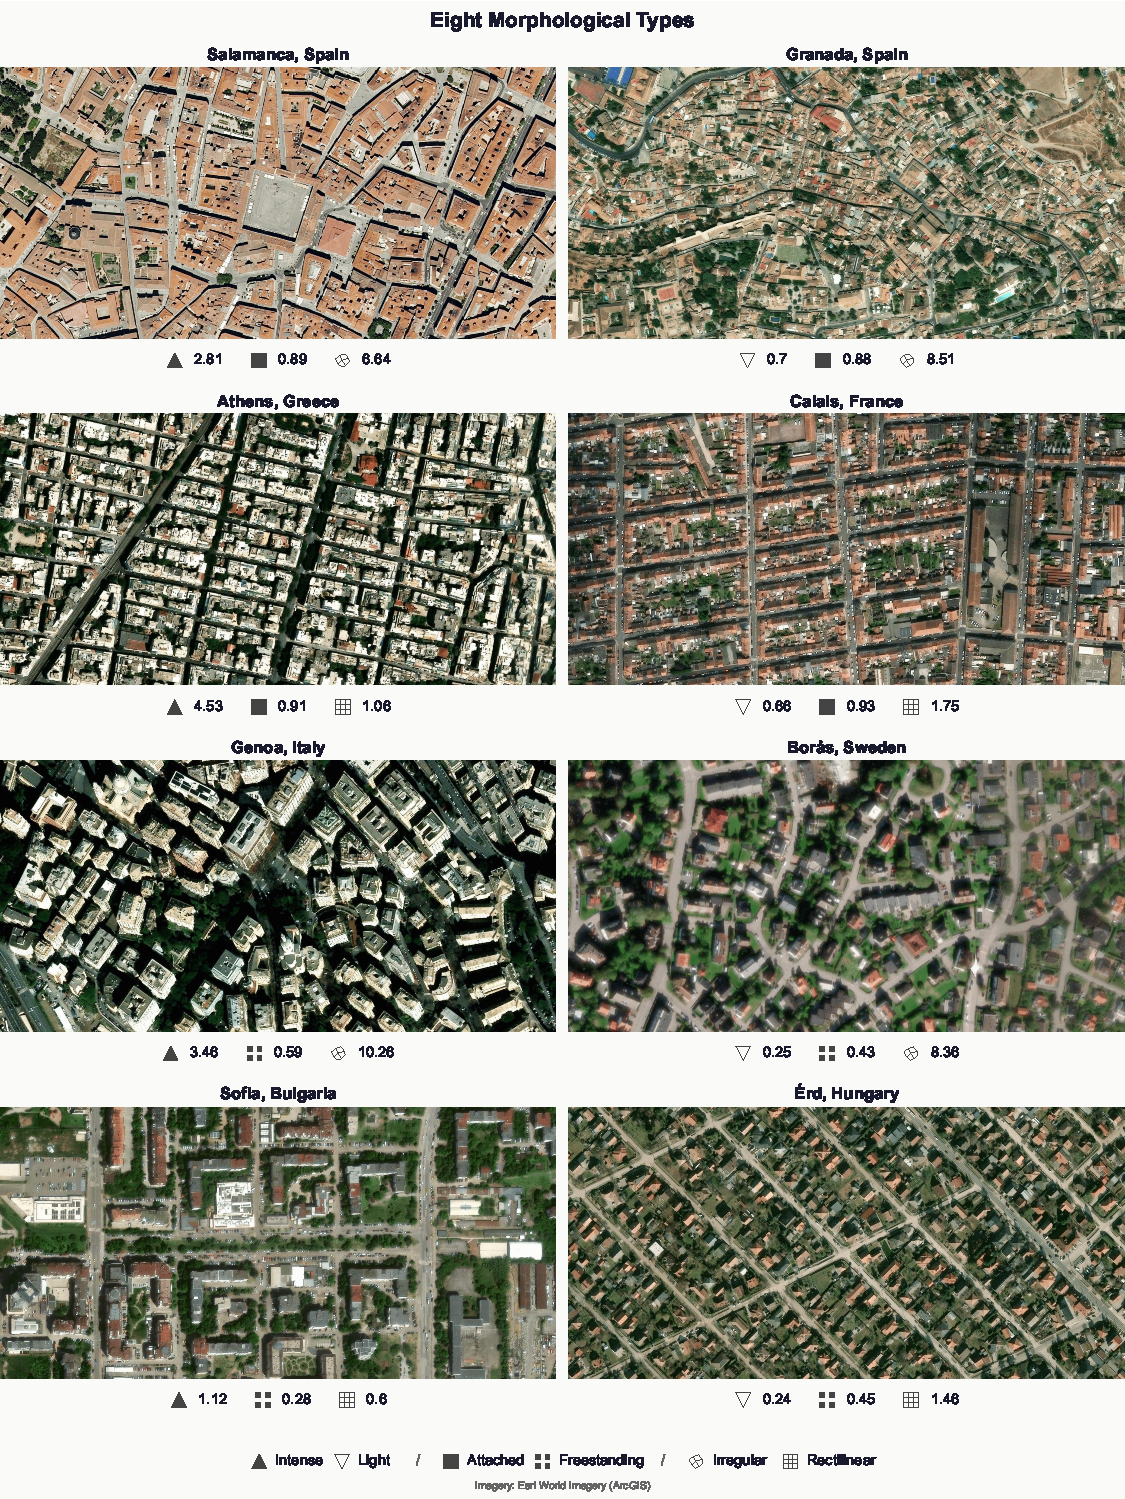
\includegraphics[width=0.98\textwidth]{outputs/atlas/plate1_exemplars.pdf}
  \caption{Satellite imagery of eight representative cities, one per morphological type.}
  \label{fig:plate1}
\end{figure}

The classification captures three independent dimensions (the mass of the built environment, its enclosure of the street, and the irregularity of its layout) whose combination yields eight types; Plate~1 (Figure~\ref{fig:plate1}) shows an exemplar city from each type. We take an intentionally simple approach, departing from the current trend towards data-heavy classification: data-driven clustering of high-dimensional morphological data yields type boundaries sensitive to algorithm and input choices \citep{berghauser2019systematic, fleischmann2022morphological}. Historical morphological traditions, by contrast, interpret urban form through hierarchies of building fabric, plot patterns, and street systems \citep{whitehand2001british, kropf2009aspects}, but these do not straightforwardly operationalise at continental scale from open data. Against this backdrop, we use a small number of building-footprint properties available across open data sources where plot or cadastral boundaries are not.

Three considerations select these axes over familiar alternatives. First, each axis is a property of the built fabric itself rather than of its occupancy or of the measurement apparatus: population density describes residents rather than form and is held out as an outcome dimension (Plates~8 and~11), while connectivity and block size are properties of the street network and are held out so that the classification remains independent of the network used to measure access (Plates~5--7). Second, the axes carry distinct information: intensity summarises how much is built, continuity how the built mass addresses the street, and irregularity how the layout is ordered, and the three are close to uncorrelated across \nClassifiedM{} million streets (\ref{sec:axis-selection}). Compactness in the Spacematrix sense (ground coverage) is not added as a fourth axis, because pairing floor-area intensity with frontage recovers the configurational distinction that ground-space index provides while discriminating types more sharply (\ref{sec:axis-selection}). Third, each axis corresponds to a lever that planning regimes control directly: permitted floor area, build-to lines and street enclosure, and plan geometry. A fixed-threshold classification is coarser than a fitted one, but it has three properties that matter here: a type label means the same thing in every city; the boundaries can be inspected and adjusted, since all thresholds are parameters of the published code; and the classification cannot absorb the network and access variables it is later used to analyse. Table~\ref{tab:positioning} situates the approach among established treatments of urban tissue.

\begin{table}[ht]
  \centering
  \caption{The SOAR-EU classification in relation to established approaches to urban form.}
  \label{tab:positioning}
  \small
  \begin{tabular}{@{}p{2.4cm}p{11.4cm}@{}}
    \toprule
    \multicolumn{2}{@{}l}{\textbf{Conzenian town-plan analysis} \citep{whitehand2001british}} \\
    \quad Unit & Plan units, plots \\
    \quad Basis & Qualitative reading of street, plot, and building layers \\
    \quad Coverage & Individual towns \\
    \quad Application & Historical explanation of townscape \\
    \addlinespace
    \multicolumn{2}{@{}l}{\textbf{Muratorian typology} \citep{caniggia2001architectural}} \\
    \quad Unit & Building type in tissue \\
    \quad Basis & Qualitative reading of type--plot--block associations \\
    \quad Coverage & Individual cities \\
    \quad Application & Typological continuity in design \\
    \addlinespace
    \multicolumn{2}{@{}l}{\textbf{Spacematrix} \citep{berghauser2010spacematrix}} \\
    \quad Unit & Block, island \\
    \quad Basis & FSI, GSI, OSR, storeys \\
    \quad Coverage & Samples of districts \\
    \quad Application & Density benchmarking in design and regulation \\
    \addlinespace
    \multicolumn{2}{@{}l}{\textbf{Numerical taxonomy and clustering} \citep{fleischmann2022morphological, dibble2019origin}} \\
    \quad Unit & Tessellation cells, sanctuary areas \\
    \quad Basis & Tens to hundreds of morphometrics, unsupervised clustering \\
    \quad Coverage & Single cities to countries \\
    \quad Application & Data-driven pattern discovery \\
    \addlinespace
    \multicolumn{2}{@{}l}{\textbf{SOAR-EU (this paper)}} \\
    \quad Unit & Street segment \\
    \quad Basis & Three interpretable axes with fixed thresholds \\
    \quad Coverage & \nCities{} urban centres, \nClassifiedM{}M streets \\
    \quad Application & Comparative description, benchmarking, monitoring \\
    \bottomrule
  \end{tabular}
\end{table}

For \emph{Intensity}, we use floor space index (FSI), computed at the level of Urban Atlas land-cover blocks as the ratio of total building floor area to block land area. Each street receives a distance-weighted mean of block values from immediately surrounding blocks. FSI is the central variable in the Spacematrix framework \citep{berghauser2010spacematrix}, which establishes building density, distinct from population density, as a multi-indicator condition whose components (intensity, compactness, spaciousness) can vary independently \citep{dovey2014urban, godoyshimizu2021density}. FSI integrates vertical extent and horizontal coverage, and discriminates between types more sharply than height or ground coverage alone (\ref{sec:axis-selection}). We adopt FSI\,=\,\threshFSI{} as the threshold separating Intense from Light types, broadly corresponding to the transition between low-rise suburban fabric and contiguous urban development in the Spacematrix typology.

For \emph{Continuity}, we measure street-frontage ratio. FSI alone is degenerate: a ten-storey tower covering 10\% of a block and a two-storey terrace covering 50\% both produce the same ratio. Spacematrix resolves this by pairing FSI with ground-space index (GSI); because this atlas operates at the street, we instead pair FSI with facade continuity: whether buildings form a continuous wall addressing the street or stand apart \citep{hamaina2012towards, vanderhaegen2017mapping}. Frontage ratio scores the fraction of each street's more-covered side that is fronted by building facades within a maximum 35\,m corridor; it is preferred over shared wall ratio because it is more robust to the ML-derived footprints predominant in parts of southern and eastern Europe (\ref{sec:source-robustness}). We set the threshold at \threshCont{}, three-quarters of the more-covered side fronted, which sits well into the upper tail of the distribution; \ref{sec:continuity-calibration} provides background on the measure and calibrates the threshold.

For \emph{Irregularity}, we use median absolute deviation (MAD) of building orientations: the degree to which buildings within the vicinity share a common alignment. Orientation regularity reflects both deliberate geometric order and topographic constraint. Orientation entropy of street networks discriminates planned from organic cities worldwide \citep{boeing2019urban}, and morphometric profiles separate historical periods of development \citep{dibble2019origin}; we measure dispersion of building orientations rather than network entropy, both because it captures finer-grained layout irregularity and because it keeps the classification independent of the network structure used to compute accessibility. The axis discriminates between planned cities (post-war Dutch grids, socialist-era Polish estates) and two distinct sources of irregularity: organic medieval growth (Liège, Brussels) and topographically constrained development (Oslo, Bergen). We set the threshold at \threshMADdeg\textdegree.

The three axes carry largely independent information; all eight types are populated, and type membership also discriminates fabric variables it was not built from: ground-space index and building height (\ref{sec:axis-selection}).

Intensity and Irregularity are aggregated over a \kernelDist\,m distance-weighted neighbourhood around each street; Continuity is measured directly from the maximum 35\,m street-side corridor. \pctNaNFSIfourHundred\% of streets lack a computable FSI within the Intensity kernel and remain unclassified. Types are named by position on each axis in Intensity--Continuity--Irregularity order: HHH denotes Intense--Attached--Irregular; LLL denotes Light--Freestanding--Rectilinear (Table~\ref{tab:types}). The thresholds are author choices intended to mark substantively meaningful breaks rather than statistically optimised splits. Table~\ref{tab:sensitivity} reports how the share of streets falling into each type responds to $\pm$20\% variation in each threshold, holding the other two fixed: the largest share drift is \sensMaxDriftFSILo\% / \sensMaxDriftFSIHi\% under the FSI perturbations, \sensMaxDriftCONTLo\% / \sensMaxDriftCONTHi\% under Continuity, and \sensMaxDriftMADLo\% / \sensMaxDriftMADHi\% under MAD, so the classification is not finely tuned to the specific thresholds adopted.

\begin{table}[ht]
  \centering
  \caption{Summary of the eight morphological types.
    Street counts and percentages are based on \nClassifiedM{} million classified streets.
  FSI, FR (frontage ratio), and MAD are per-type medians.}
  \label{tab:types}
  \small
  \begin{tabular}{llrrrrr}
    \toprule
    Code & Type name & Streets (M) & \% & FSI & FR & MAD ($^{\circ}$) \\
    \midrule
    HHH & Intense--Attached--Irregular      & \octHHHcountM & \octHHHpct & \octHHHfsi & \octHHHcont & \octHHHmad \\
    HHL & Intense--Attached--Rectilinear    & \octHHLcountM & \octHHLpct & \octHHLfsi & \octHHLcont & \octHHLmad \\
    HLH & Intense--Freestanding--Irregular  & \octHLHcountM & \octHLHpct & \octHLHfsi & \octHLHcont & \octHLHmad \\
    HLL & Intense--Freestanding--Rectilinear & \octHLLcountM & \octHLLpct & \octHLLfsi & \octHLLcont & \octHLLmad \\
    LHH & Light--Attached--Irregular        & \octLHHcountM & \octLHHpct & \octLHHfsi & \octLHHcont & \octLHHmad \\
    LHL & Light--Attached--Rectilinear      & \octLHLcountM & \octLHLpct & \octLHLfsi & \octLHLcont & \octLHLmad \\
    LLH & Light--Freestanding--Irregular    & \octLLHcountM & \octLLHpct & \octLLHfsi & \octLLHcont & \octLLHmad \\
    LLL & Light--Freestanding--Rectilinear  & \octLLLcountM & \octLLLpct & \octLLLfsi & \octLLLcont & \octLLLmad \\
    \bottomrule
  \end{tabular}
\end{table}

\begin{table}[ht]
  \centering
  \caption{Type share (\%) under $\pm$20\% threshold perturbation, by axis. Baseline thresholds: FSI = \threshFSI, Continuity = \threshCont, MAD = \threshMADdeg\textdegree.}
  \label{tab:sensitivity}
  \small
  % Auto-generated by generate_macros.py — do not edit by hand.
\begin{tabular}{llrrr}
\toprule
Axis & Type & $-20\%$ share (\%) & Baseline (\%) & $+20\%$ share (\%) \\
\midrule
FSI & HHH & 2.7 & 2.2 & 1.9 \\
 & HHL & 5.1 & 4.1 & 3.4 \\
 & HLH & 5.9 & 4.3 & 3.3 \\
 & HLL & 11.3 & 7.9 & 5.8 \\
 & LHH & 2.9 & 3.3 & 3.7 \\
 & LHL & 6.7 & 7.7 & 8.4 \\
 & LLH & 23.8 & 25.4 & 26.5 \\
 & LLL & 41.7 & 45.0 & 47.1 \\
\midrule
CONT & HHH & 3.0 & 2.2 & 1.2 \\
 & HHL & 5.4 & 4.1 & 2.1 \\
 & HLH & 3.6 & 4.3 & 5.3 \\
 & HLL & 6.6 & 7.9 & 9.9 \\
 & LHH & 6.1 & 3.3 & 1.4 \\
 & LHL & 13.5 & 7.7 & 3.1 \\
 & LLH & 22.7 & 25.4 & 27.4 \\
 & LLL & 39.2 & 45.0 & 49.6 \\
\midrule
MAD & HHH & 2.7 & 2.2 & 1.8 \\
 & HHL & 3.6 & 4.1 & 4.5 \\
 & HLH & 5.2 & 4.3 & 3.6 \\
 & HLL & 7.1 & 7.9 & 8.6 \\
 & LHH & 4.1 & 3.3 & 2.7 \\
 & LHL & 6.9 & 7.7 & 8.3 \\
 & LLH & 30.6 & 25.4 & 21.1 \\
 & LLL & 39.9 & 45.0 & 49.4 \\
\bottomrule
\end{tabular}

\end{table}

% ==============================================================================
\section{Plates 2 \& 3 --- Continental Distribution of the Types}
\label{sec:plate2}
% ==============================================================================

\begin{figure}[p]
  \centering
  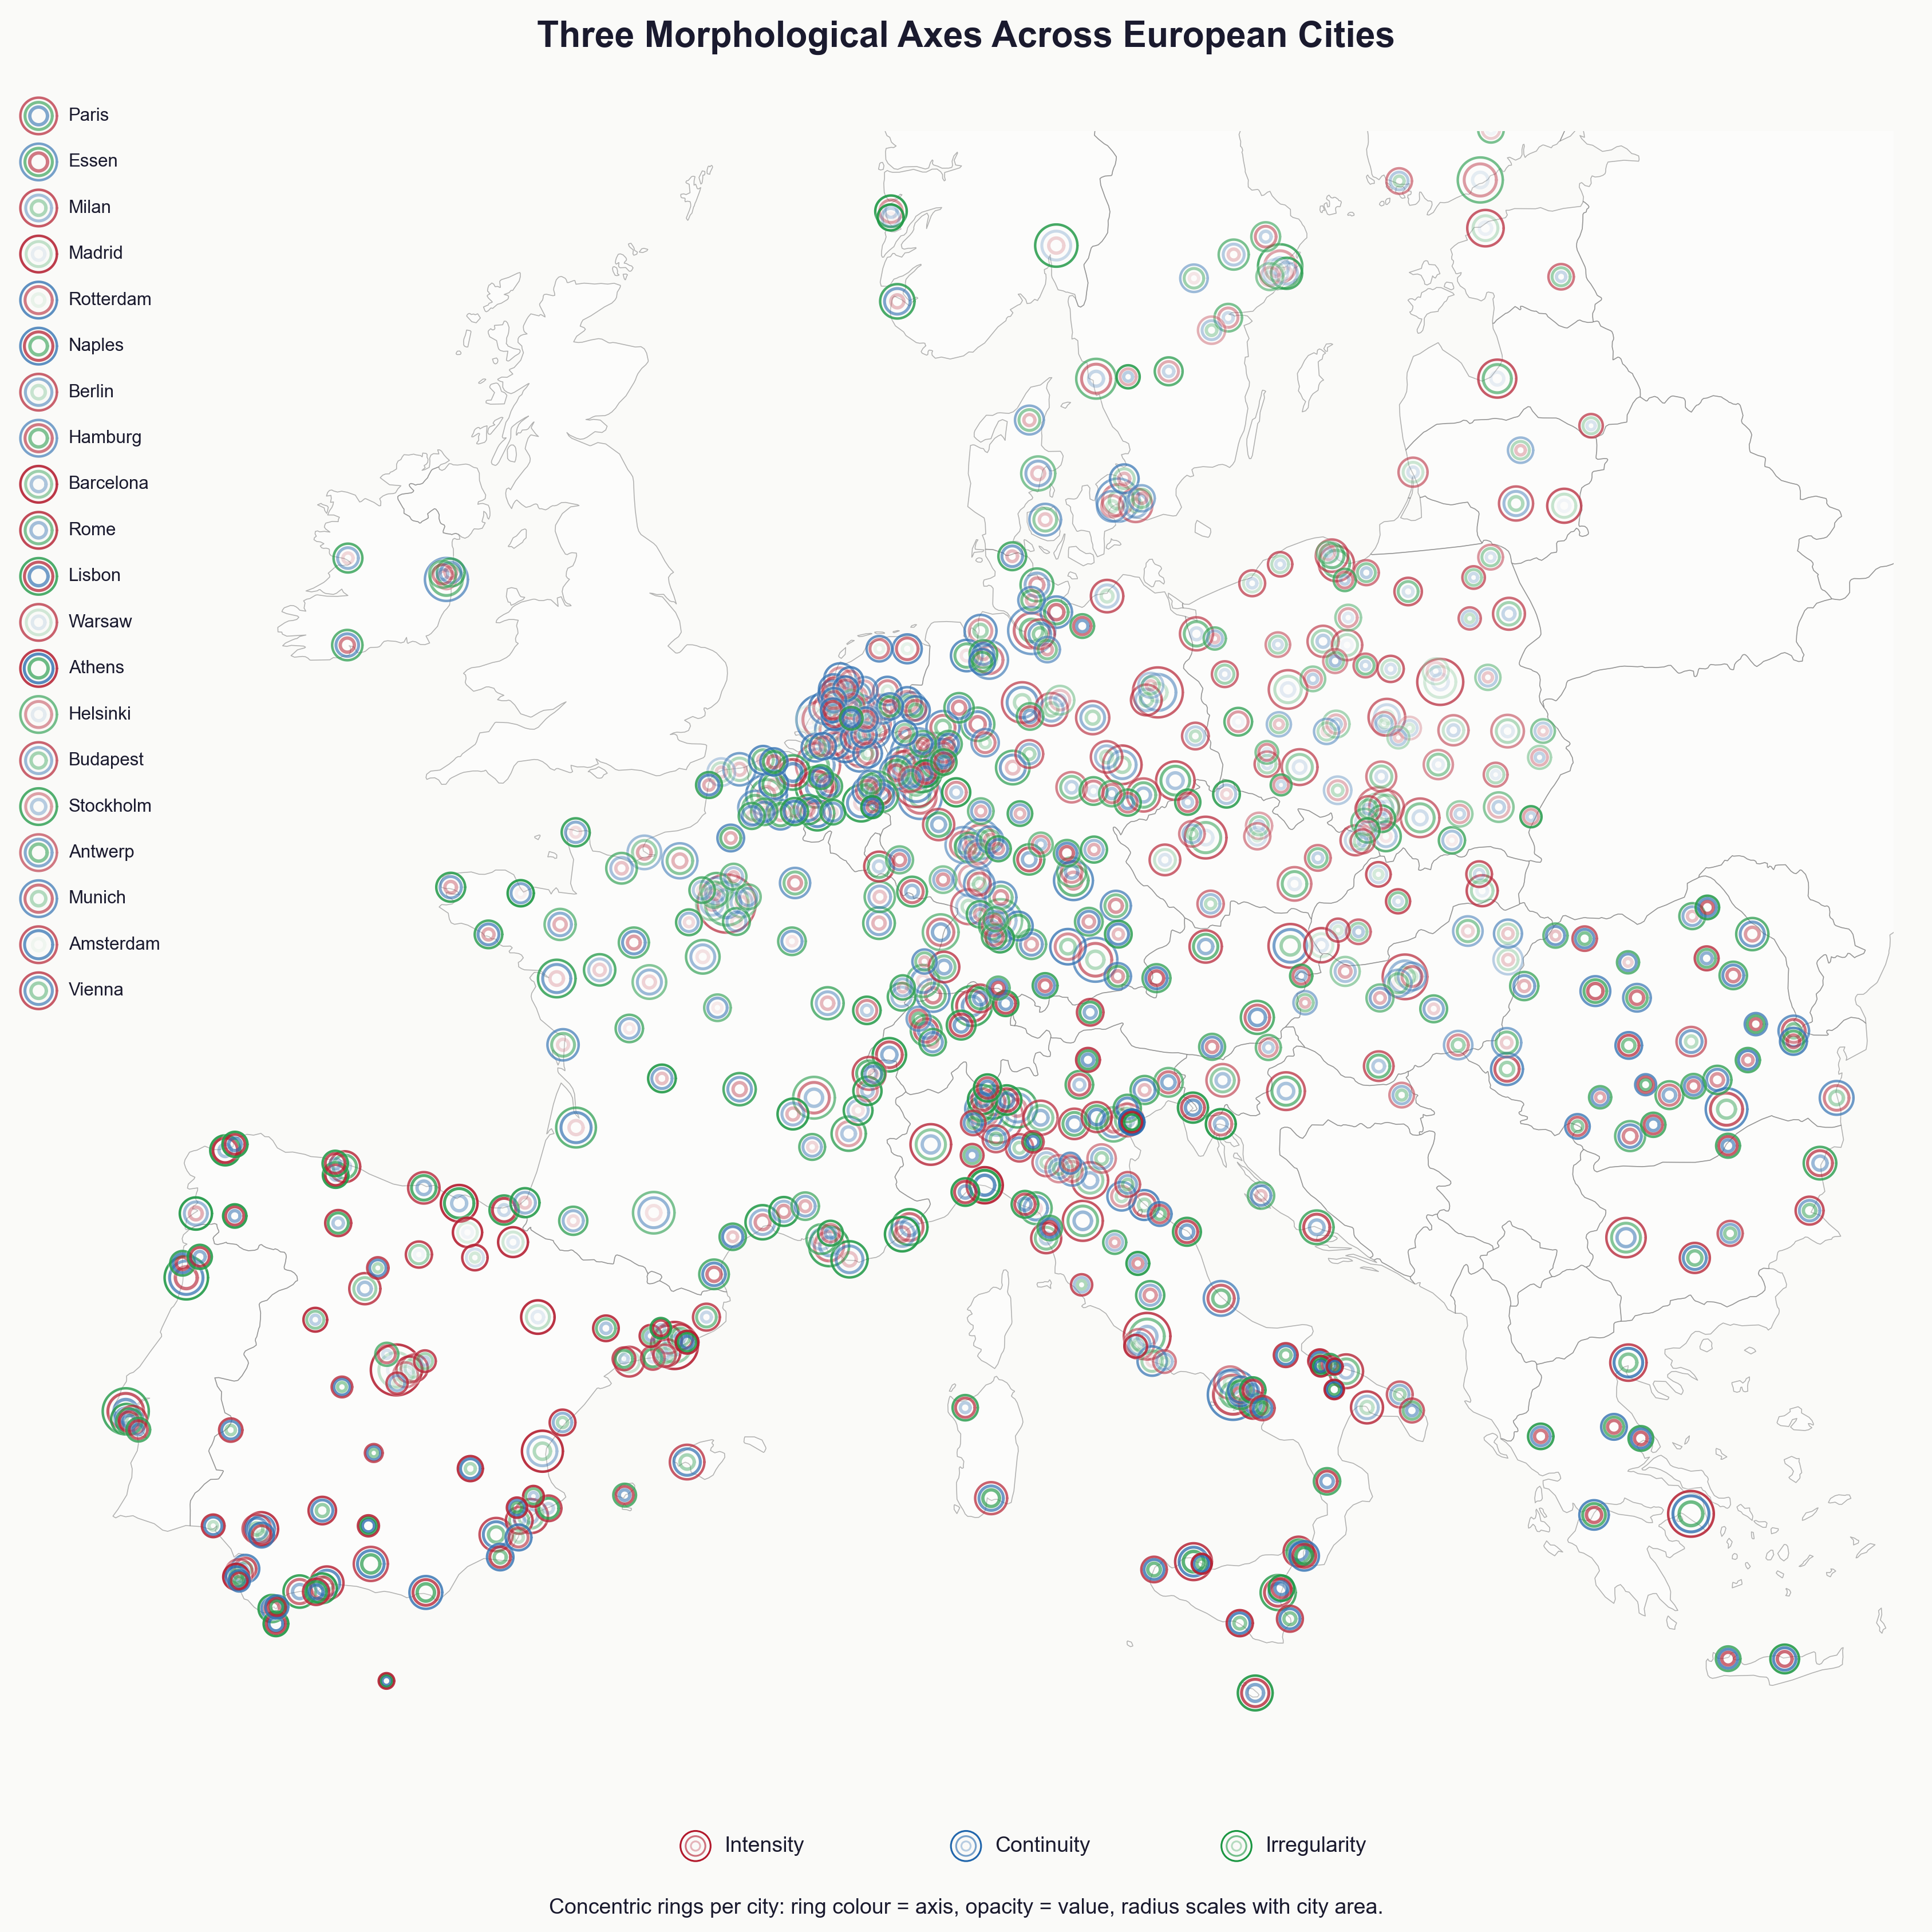
\includegraphics[width=\textwidth]{outputs/atlas/plate2_ripples.png}
  \caption{Continental ring map: three morphological axes across \nCities{} cities. Each city is drawn as three concentric rings, one per axis (colour-coded). For each city, rings are ordered by value (the axis with the lowest score sits innermost, the highest outermost), and opacity scales with value, so low-value axes collapse towards the centre and fade while high-value axes push outward and appear solid. Cluster size scales with city area.}
  \label{fig:plate2}
\end{figure}

\begin{figure}[tb]
  \centering
  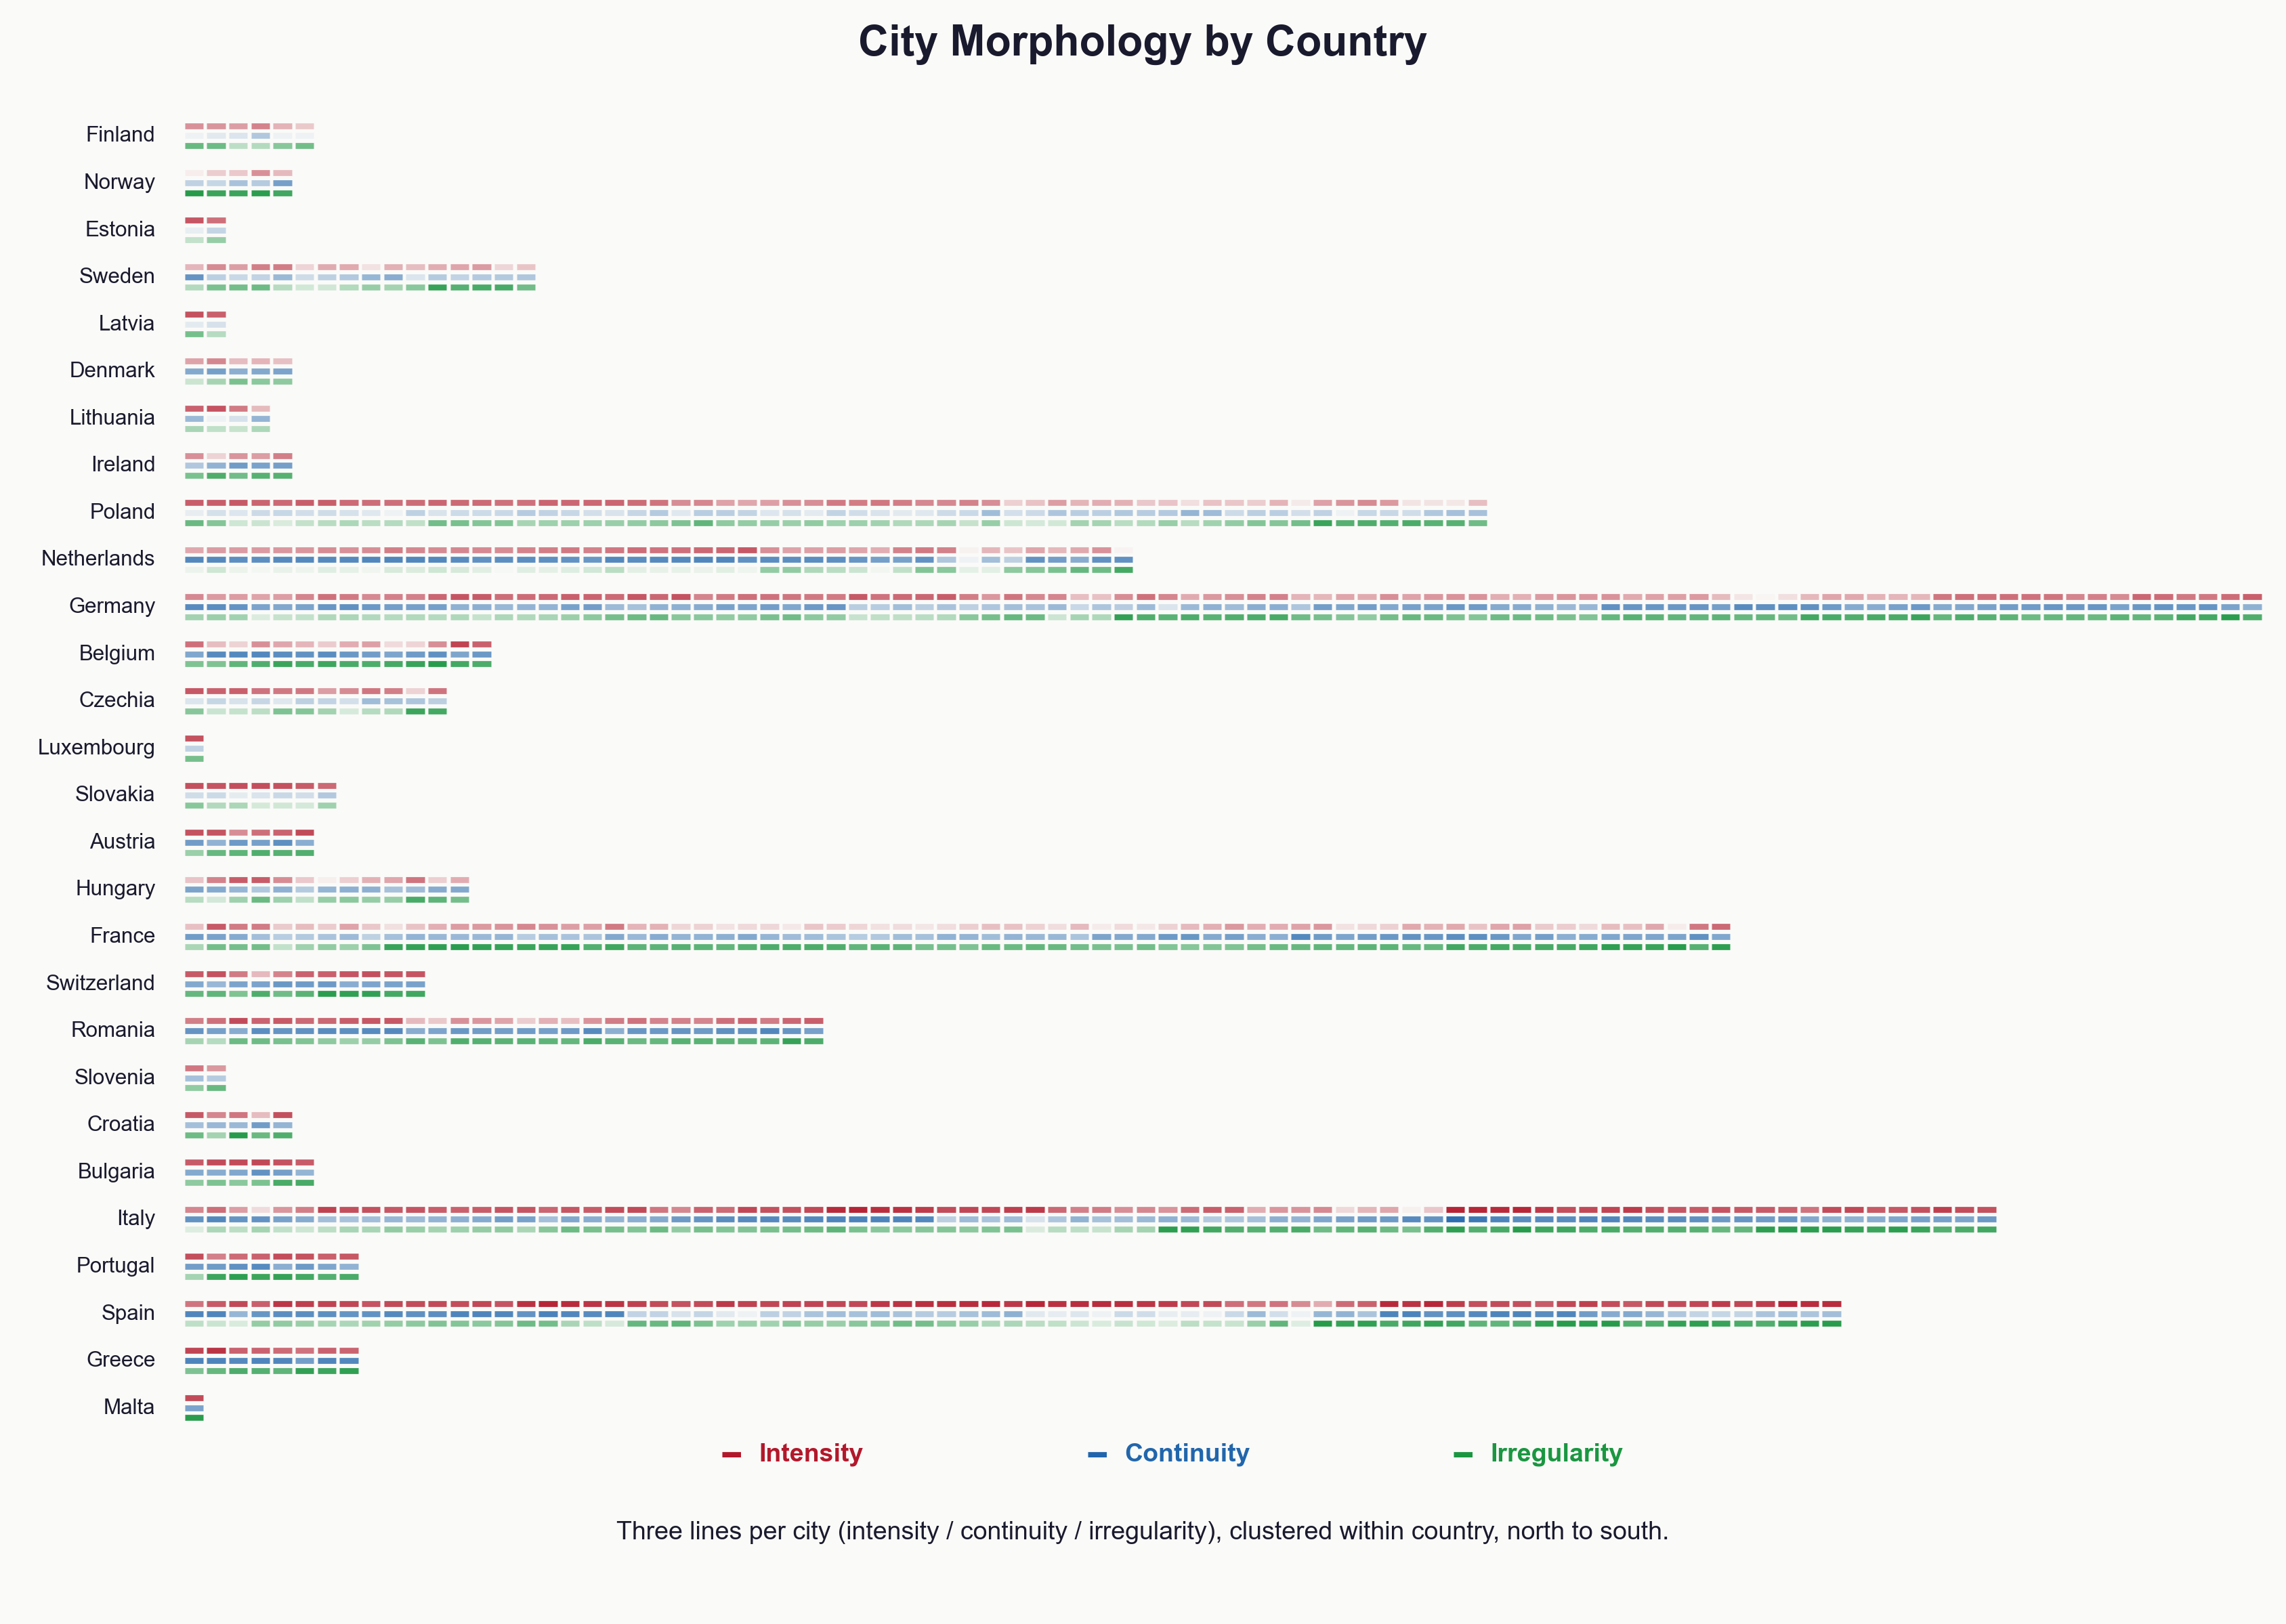
\includegraphics[width=\textwidth]{outputs/atlas/plate3_lines.png}
  \caption{Three-axis country profiles, cities ordered north to south. Each line plots one city's value on one axis (colour-coded); line opacity scales with value, so solid lines mark high-value axes and faint lines low-value axes.}
  \label{fig:plate3}
\end{figure}

Plate~2 (Figure~\ref{fig:plate2}) maps the three axes across Europe at city level using concentric rings; Plate~3 (Figure~\ref{fig:plate3}) disaggregates the same data into country-grouped line profiles. Three broad bands emerge. A \emph{Southern European} band is characterised by high Intensity: Spain has the highest country-median FSI in the sample (\fsiCtryES; Barcelona \fsiBarcelona, Madrid \fsiMadrid), and the band continues through Portugal, Italy, and Austria to Greece, where Athens reaches \fsiAthens. These high floor-area ratios share a morphological outcome (four- to six-storey structures on dense blocks) but arise from distinct national mechanisms. In Spain, nineteenth-century \emph{ensanche} grids permitted deep-lot perimeter blocks whose interior courtyards were progressively filled as twentieth-century legislation raised allowable floor-area ratios \citep{busquets2005barcelona}. In Greece, the \emph{antiparochi} system drove parcel-by-parcel vertical densification across Athens from the 1950s, producing near-total ground coverage through a financial mechanism rather than a planning intention \citep{maloutas2003promoting}. City-level Continuity varies across the band (Spain's country median is \contCtryES{} against Greece's \contCtryEL{}, the highest in the sample), and city medians understate within-city variation: \pctContBarcelona\% of Barcelona's streets and \pctContAthens\% of Athens's exceed the Attached threshold, concentrated in dense historic cores.

A second, \emph{Eastern European} band shows comparable Intensity through a different building stock: Bulgaria, Slovakia, and the Baltic states reach comparable building mass through freestanding apartment blocks and housing estates, fabric that withdraws from the street despite comparable floor-area ratios. Intensity and street enclosure are largely independent at continental scale. The third band is a \emph{Western European} Continuity signature: the Netherlands and Belgium share elevated frontage ratios (NL: $\sim$\contNLmed; BE: $\sim$\contBEmed), consistent with a common Low Countries tradition of terraced and semi-detached dwellings with party walls; within Amsterdam, \pctContAmsterdam\% of streets exceed the Attached threshold, within Brussels \pctContBrussels\%.

The resemblance between the Netherlands and Belgium ends at Continuity. Dutch cities are among the most regular in the sample (median MAD \madNLmed\textdegree), reflecting a strongly plan-led tradition of detailed, binding local land-use plans \citep{faludi1994rule}, reinforced by reclaimed polder land whose rectilinear drainage geometry is echoed in subsequent street layouts. Belgian cities combine near-identical attachment with considerably higher irregularity (median MAD \madBEmed\textdegree), the product of a permissive building-permit regime and individual-plot self-construction along rural roads, a pattern known as \emph{lintbebouwing} \citep{dedecker2008facets}. Within countries, finer gradients reflect topography, wartime disruption, and housing traditions: Norway combines high Irregularity with low Intensity (freestanding buildings on layouts dictated by slopes and valleys), while Portugal and Switzerland pair similar topographically driven Irregularity with greater building mass; Italy's Intensity climbs from north to south but its morphological character remains broadly consistent across the peninsula; Germany's Continuity ranges widely, consistent with divergent post-war reconstruction strategies \citep{diefendorf1993wake}.

% ==============================================================================
\section{Plate 4 --- Building Form and Street Enclosure}
\label{sec:plate4}
% ==============================================================================

\begin{figure}[p]
  \centering
  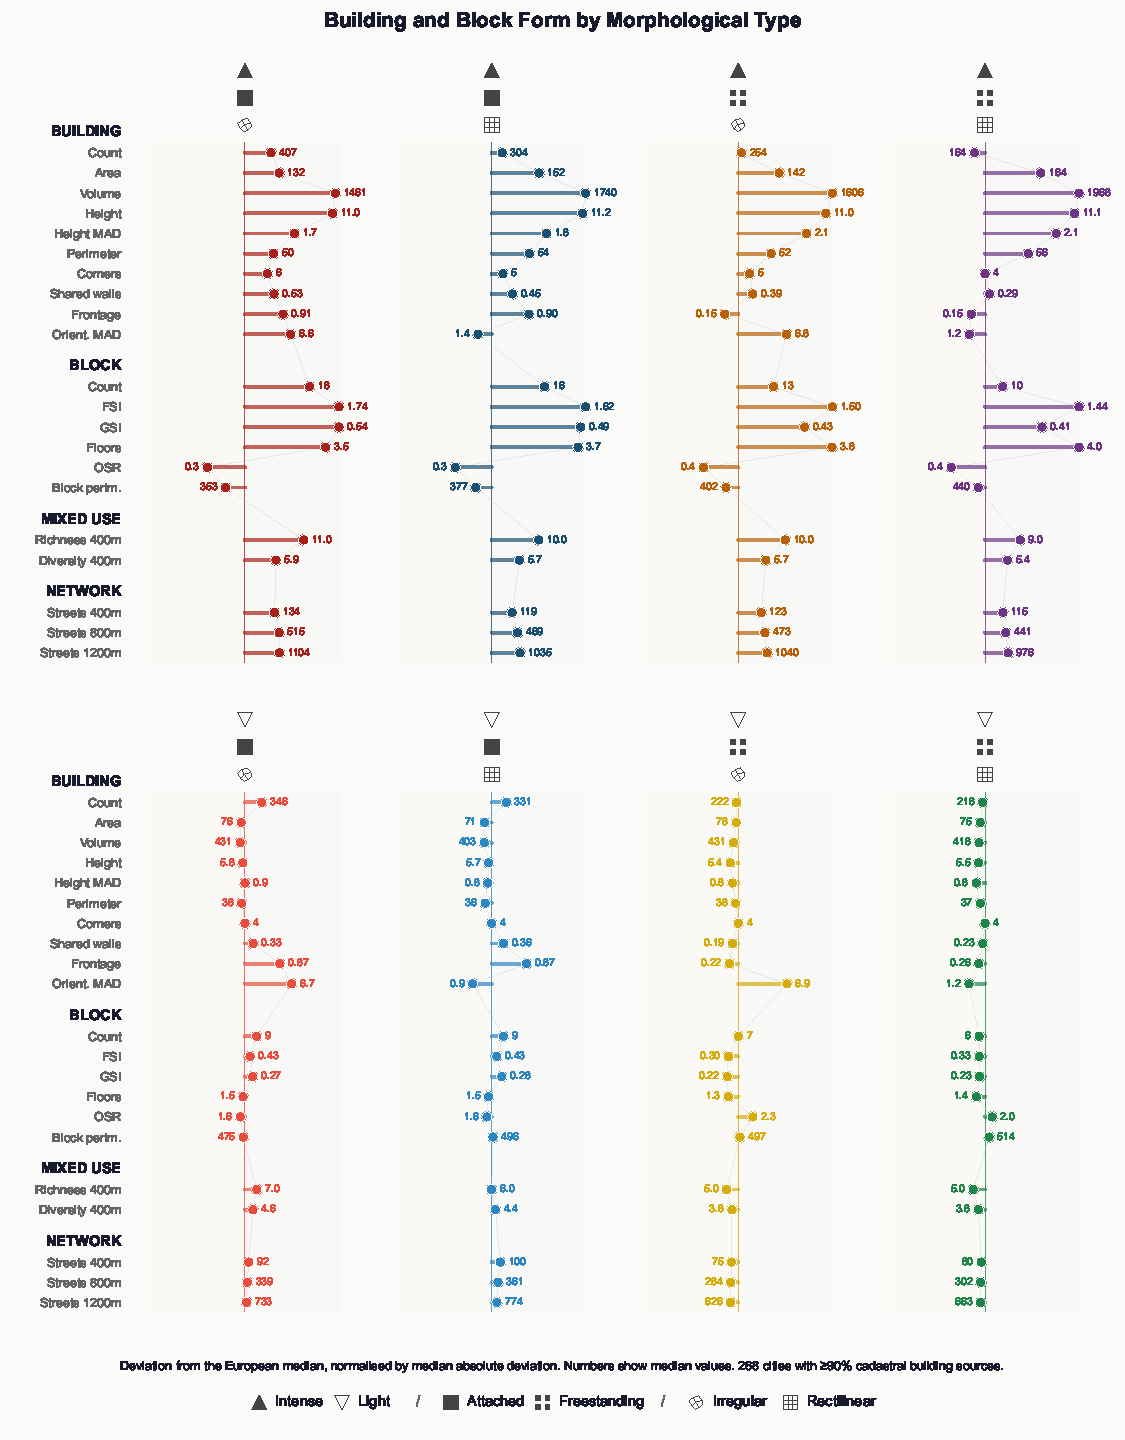
\includegraphics[width=\textwidth]{outputs/atlas/plate4_buildings.pdf}
  \caption{Building, block, and network morphometrics across the eight types, restricted to \nMLRestrictedCities{} cities with less than 10\% ML-derived building footprints (see \ref{sec:source-robustness}). The full \nCities-city version is provided in the Supplementary Material (Figure~\ref{fig:plate4_full}).}
  \label{fig:plate4}
\end{figure}

Plate~4 (Figure~\ref{fig:plate4}) compares building and block indicators (GSI, FSI, open-space ratio [OSR], mean floors), landuse richness, and network density across the eight types, as deviations from the European median.

The Intense types contrast two strategies for accommodating building mass. Intense--Attached (HHH, HHL) are the continuous perimeter-block tissues characteristic of the pre-modern and nineteenth-century European city \citep{panerai2004urban}: high floor area on small blocks, with articulated building plans (bays, setbacks, light wells), as in Barcelona's \emph{ensanche}, Parisian \emph{arrondissements}, and central Amsterdam. Intense--Freestanding (HLH, HLL) reach comparable intensity through a different strategy: fewer, larger buildings with simpler plans set in open space (open-space ratio \octHLHosr--\octHLLosr{} against \octHHHosr{} in HHH). This form is associated with modernist housing estates (slab blocks and point towers in open space) and with post-war reconstruction and socialist-era planned development \citep{stanilov2007post}. The divide broadly reflects the historical shift from pre-modern fabric to mid-twentieth-century development, where the street's role as connective tissue was de-emphasised.

The Light types divide along the same Continuity axis but at lower mass. LHH and LHL (Light--Attached) encompass the suburban terraced house, semi-detached villa, and low-rise row dwelling found across the Netherlands, Belgium, and many German cities: many small buildings forming near-continuous frontage at modest height. LLH and LLL are Light--Freestanding: detached houses on individual plots, the predominant fabric of peripheral and suburban Europe. LLL alone accounts for \octLLLpct\% of all classified streets, and the four Light types together for \pctLightTypes\%. The network thins with mass: an HHH street reaches nearly twice as many other streets within \kernelDist\,m as an LLH one.

Two landuse-mix measures characterise commercial categories near each street: Hill $q_0$ (richness) counts distinct point-of-interest categories within \kernelDist\,m, and Hill $q_1$ (Shannon diversity) weights by category balance. Both are highest in Intense--Attached fabric, which combines building mass with continuous ground-floor frontage, and lowest in Light--Freestanding. Types with only one of the two conditions fall between: Intense--Freestanding estates supply mass without continuous frontage, while Light--Attached terraces supply frontage without mass.

% ==============================================================================
\section{Plates 5, 6 \& 7 --- Service Access from the Street}
\label{sec:plate5}
% ==============================================================================

\begin{figure}[htp]

  \centering
  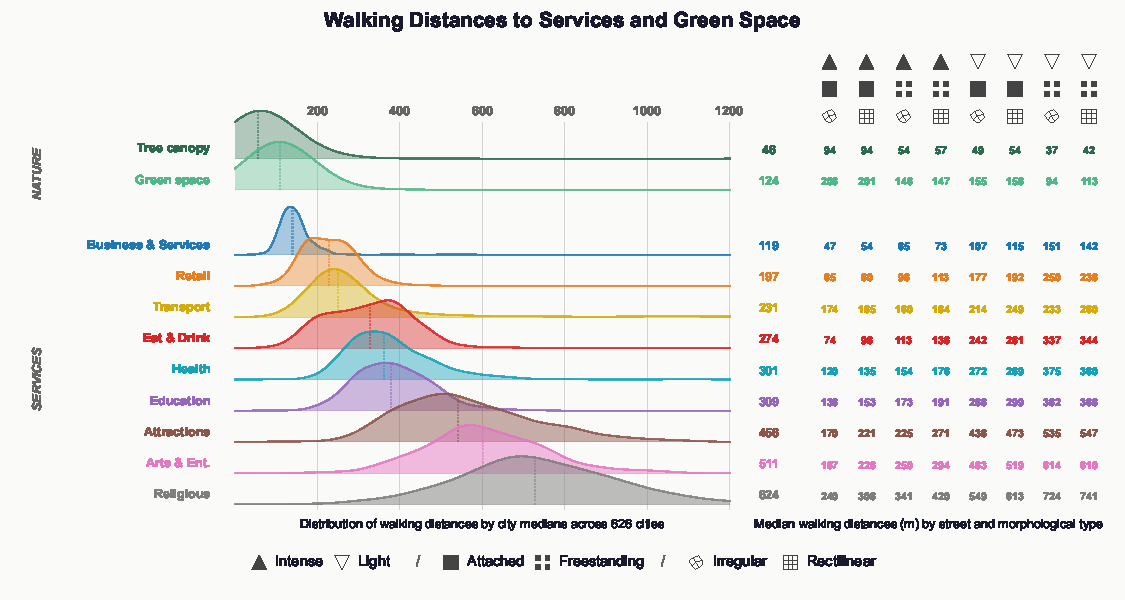
\includegraphics[width=\textwidth]{outputs/atlas/plate5_access.pdf}
  \caption{Walking distances to services and green space, by category and morphological type.}
  \label{fig:plate5}
\end{figure}

These three plates examine three dimensions of service access from each street: the median walking distance to the nearest facility in each category (Plate~5, Figure~\ref{fig:plate5}); the fraction of streets with no facility within walking distance (Plate~6, Figure~\ref{fig:plate6}); and the within-type spread of the first measure (Plate~7, Figure~\ref{fig:plate7}). All three vary systematically across the eight morphological types, and the gradient runs in opposite directions for commercial services and green space.

The continental ranking of median distances places trees closest, followed by business \& services, green space, retail, transport, eat \& drink, health, and education; the discretionary categories (attractions, arts, religious) are farthest of all. The type gradient is steepest for retail and eat \& drink, the categories most dependent on foot traffic and ground-floor premises. From HHH to LLL, retail grows from \octHHHretail\,m to \octLLLretail\,m (a \retailFoldHHHtoLLL-fold difference) and eat \& drink from \svcEatdrinkHHH\,m to \svcEatdrinkLLL\,m (a \eatDrinkFoldHHHtoLLL-fold gap). Because LLL is the most common type, the longer distance applies to more streets than the shorter one.

\begin{figure}[htp]

  \centering
  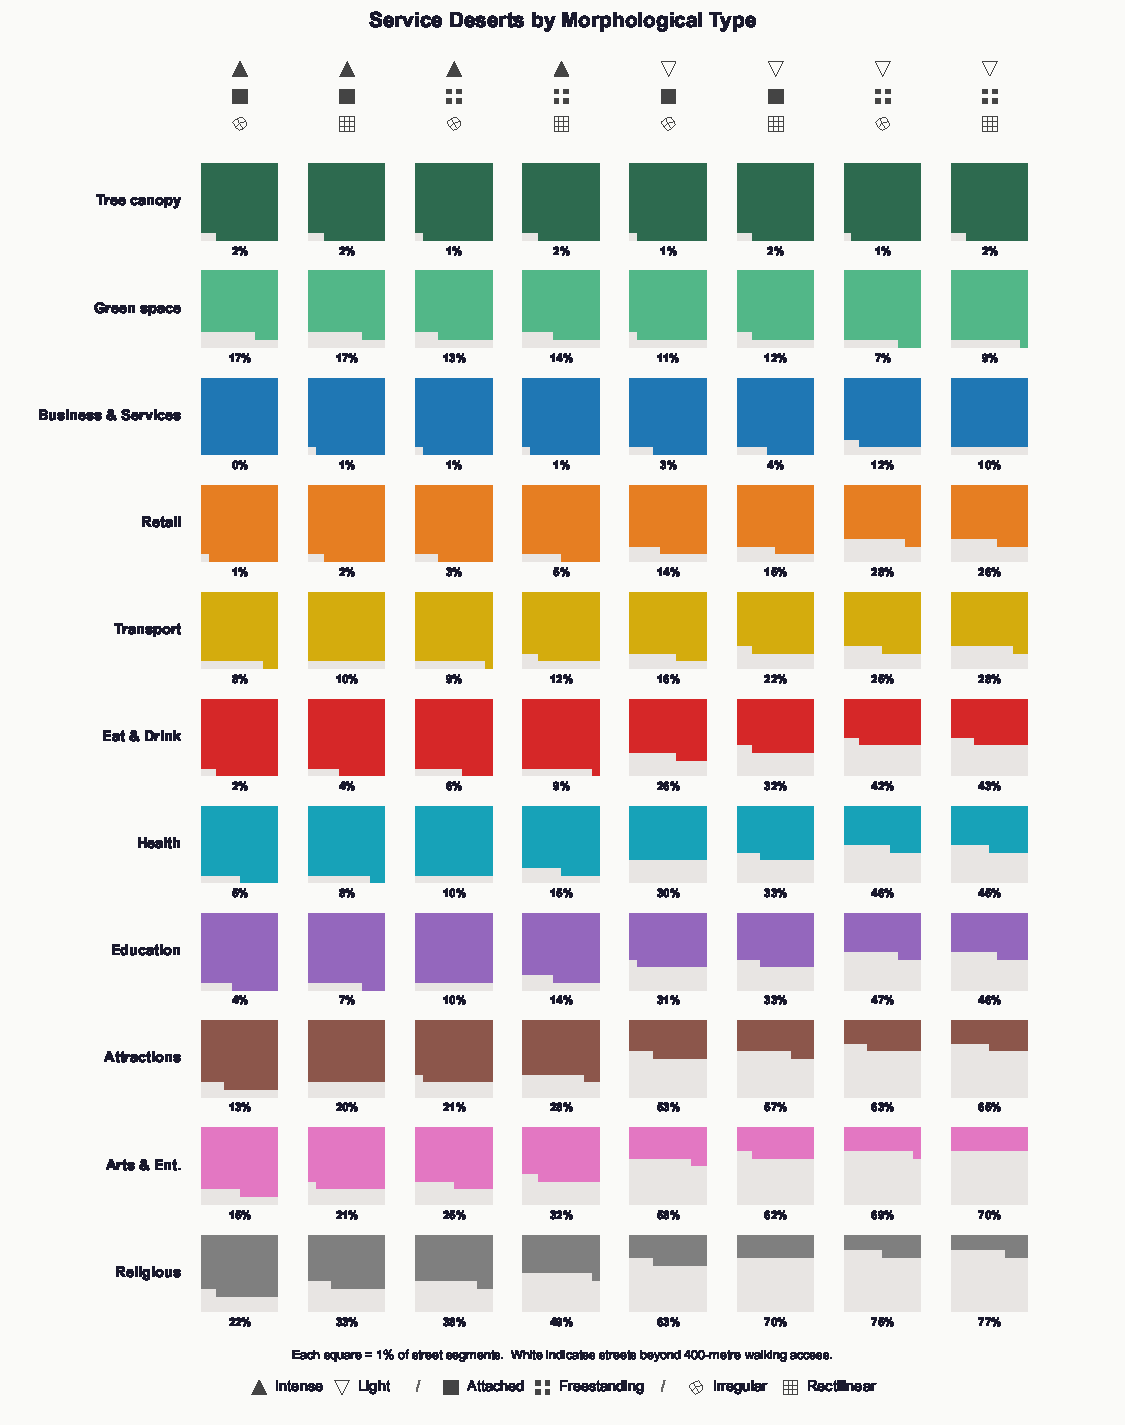
\includegraphics[width=\textwidth]{outputs/atlas/plate6_service_desert.pdf}
  \caption{Service deserts: percentage of streets with no service within \serviceCatchment\,m walking distance.}
  \label{fig:plate6}
\end{figure}

Within \serviceCatchment\,m, roughly five minutes at average walking speed, commercial deserts show that the Continuity axis carries an effect independent of Intensity. In HHH, \desertRetailHHH\% of streets lack retail; in the otherwise similar but Freestanding HLH, the figure is already \desertRetailHLH\%. At Light Intensity the split widens: LHH has \desertRetailLHH\% retail deserts versus \desertRetailLLH\% in LLH, with facade continuity roughly halving the desert fraction at constant Intensity. The same gradient holds for eat \& drink (\desertEatDrinkHHH\% to \desertEatDrinkLLH\%), health \& medical (\desertHealthHHH\% to \desertHealthLLH\%), and education (\desertEducationHHH\% to \desertEducationLLH\%). Within-type spreads (Plate~7) amplify the same gradient: the retail interquartile range (IQR) roughly triples from \iqrRetailHHH\,m in HHH to \iqrRetailLLH\,m in LLH, with the types farthest from services also the least consistent.

\begin{figure}[htp]

  \centering
  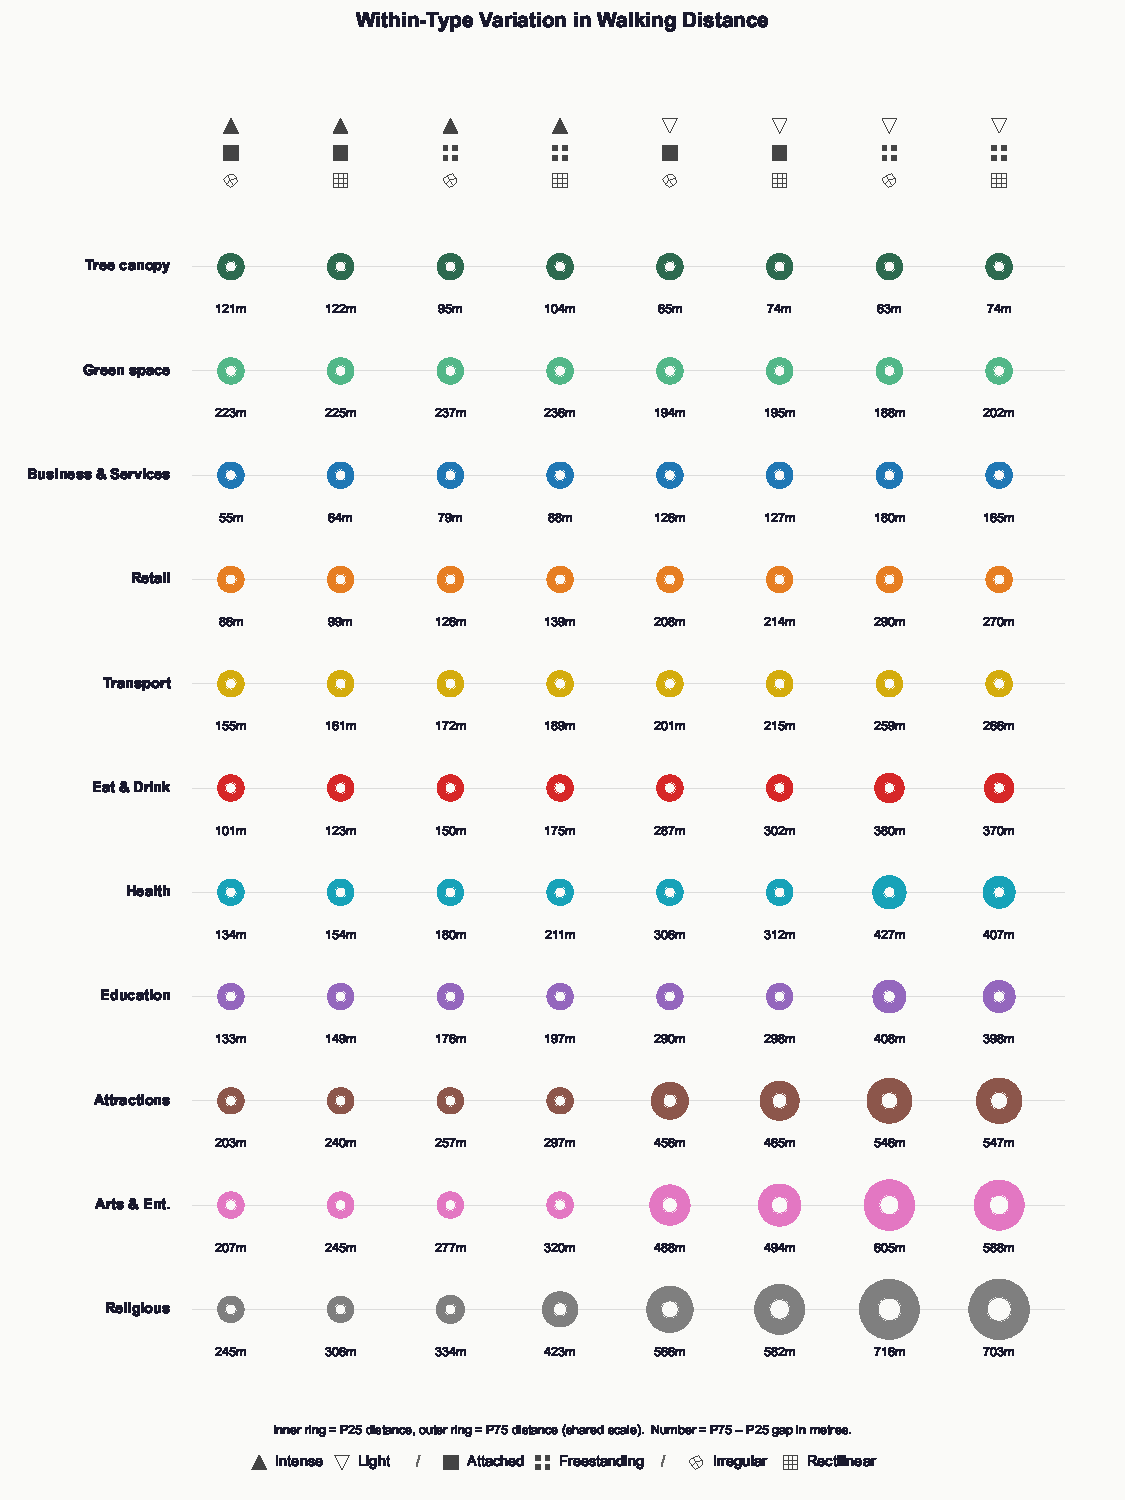
\includegraphics[width=\textwidth]{outputs/atlas/plate7_unevenness.pdf}
  \caption{Within-type variation in walking distance: interquartile range by type and category.}
  \label{fig:plate7}
\end{figure}

Green space reverses the gradient on every dimension. Intense types are farther from green space (\svcGreenHHH\,m in HHH versus \svcGreenLLH\,m in LLH, roughly double), have higher green-space desert fractions (\desertGreenHHH\% in both HHH and HHL versus \desertGreenLLH--\desertGreenLLL\% in LLH--LLL), and show wider within-type spreads. This inversion spans a substantially smaller range than the commercial gradient, however: the green-space difference between Intense and Light fabric is approximately twofold, against the \retailFoldHHHtoLLL-fold retail difference from HHH to LLL. Intense--Freestanding types illustrate the distinction: they carry moderate OSR (\octHLHosr--\octHLLosr) and the most open ground among the Intense types, yet their green-space desert fraction (\desertGreenHLH\% in both HLH and HLL) sits only modestly below HHH--HHL and above every Light type, because block-level open ground is not necessarily designated green space reachable by the walking network. This case carries a broader implication for the assumed trade-off between compactness and green access. If reachable green space followed residual open ground, these estates would approach the Light types' figures; they do not. Reachable green space behaves as a provision decision rather than a by-product of low building coverage, which is consistent with the weakening of the compactness--green trade-off at the city level (Plate~12): where planning allocates green space and connects it to the walking network, compact fabric reaches it. Tree canopy is the one feature distributed evenly: \desertTreesLHH--\desertTreesHLL\% of streets lack a tree-canopy polygon within \serviceCatchment\,m regardless of type. Tree exposure here refers to proximity to tree-canopy polygons from the Copernicus Street Tree Layer, not to individual street trees, which are not mapped as discrete points in this dataset.

Discretionary services depend on city-centre catchments and visitor footfall: even in HHH, \desertArtsHHH\% of streets lack an arts facility and \desertReligiousHHH\% lack a religious facility within \serviceCatchment\,m. The overall desert pattern is sharply asymmetric. In HHH, desert fractions are single digits for all but green space and the most discretionary categories. In LLL, deserts exceed 40\% for eat \& drink, health, and education, and reach 70\% or more for arts and religious facilities. Because the four Light types together account for \pctLightTypes\% of classified streets, the longer walks and higher absence rates apply to most of the European street network.

% ==============================================================================
\section{Plate 8 --- Demographics by Morphological Type}
\label{sec:plate8}
% ==============================================================================

\begin{figure}[htp]

  \centering
  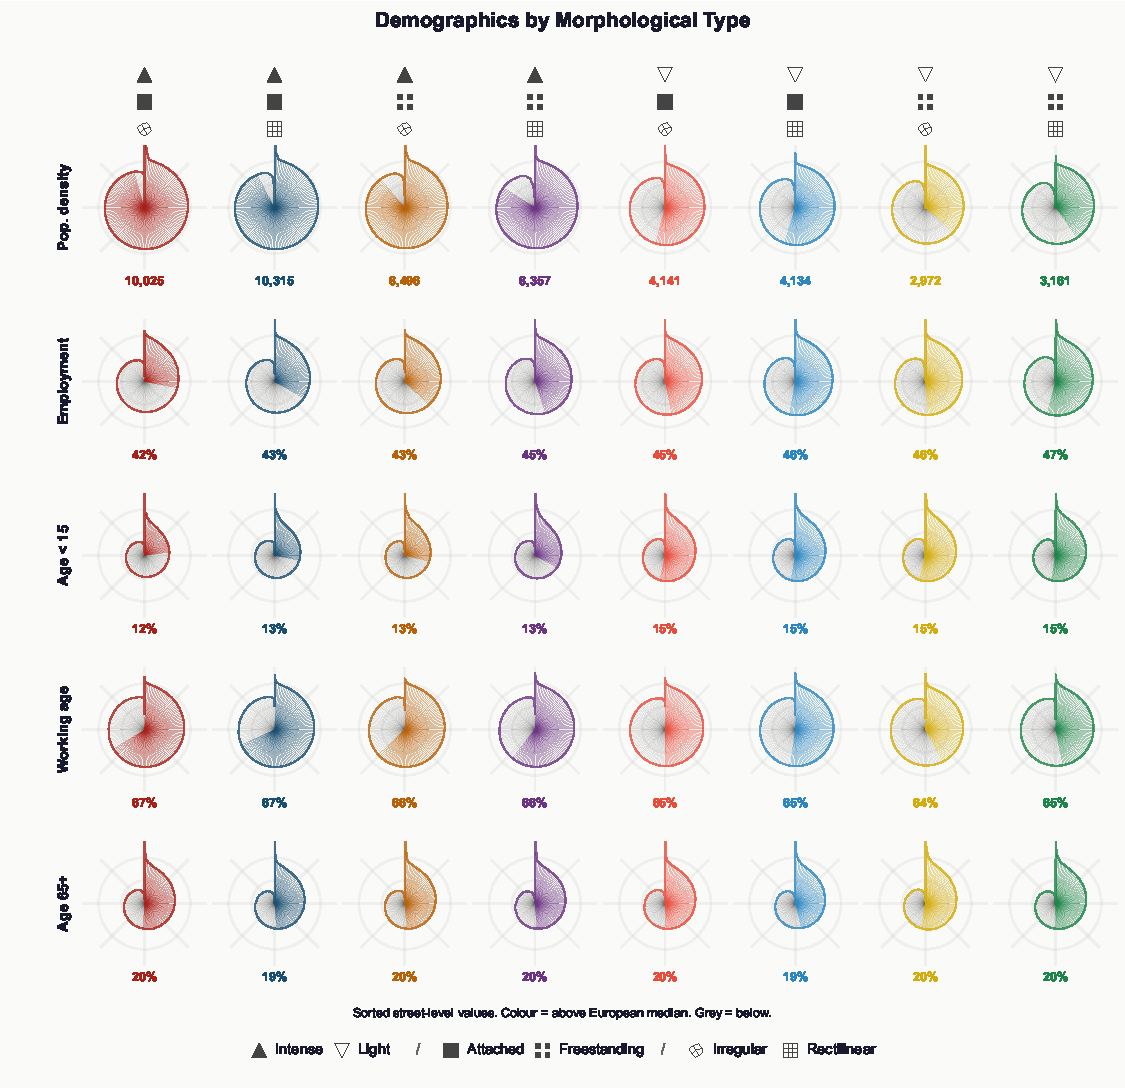
\includegraphics[width=\textwidth]{outputs/atlas/plate8_demographics.pdf}
  \caption{Demographics by morphological type: population density, employment, and age structure.}
  \label{fig:plate8}
\end{figure}

Plate~8 (Figure~\ref{fig:plate8}) cross-tabulates five demographic dimensions from the Eurostat Census Grid against the eight types. The census data are interpolated to streets from 1\,km$^2$ grid cells and describe neighbourhood-scale composition rather than dwelling-level occupancy.

Population density varies more than threefold across types and tracks built intensity: every Intense type has a median of at least \num{\popDensIntenseMin}/km$^2$ and every Light type at most \num{\popDensLightMax}, with no overlap between the two groups. Light types host more children (\youthLight\% under 15 versus \youthIntense\% in Intense types) and a correspondingly smaller working-age share, which peaks in the Intense--Attached types; the elderly share, by contrast, is relatively flat across types (\elderlyMin--\elderlyMax\%).
These higher child shares coincide with the longest service distances and highest absence rates (Plates~5--6). At least three mechanisms could produce this juxtaposition: family-sized and affordable dwellings concentrate in Light fabric; households sort into that fabric at the child-rearing stage of life; and service providers locate by purchasing density rather than by child density. Adjudicating between them is beyond the scope of this atlas, but the dataset supports first tests of each, and the discussion (Section~\ref{sec:discussion}) outlines how.

% ==============================================================================
\section{Plates 9 \& 10 --- Continental Gradients and Paired Comparisons}
\label{sec:plate9}
% ==============================================================================

\begin{figure}[htp]

  \centering
  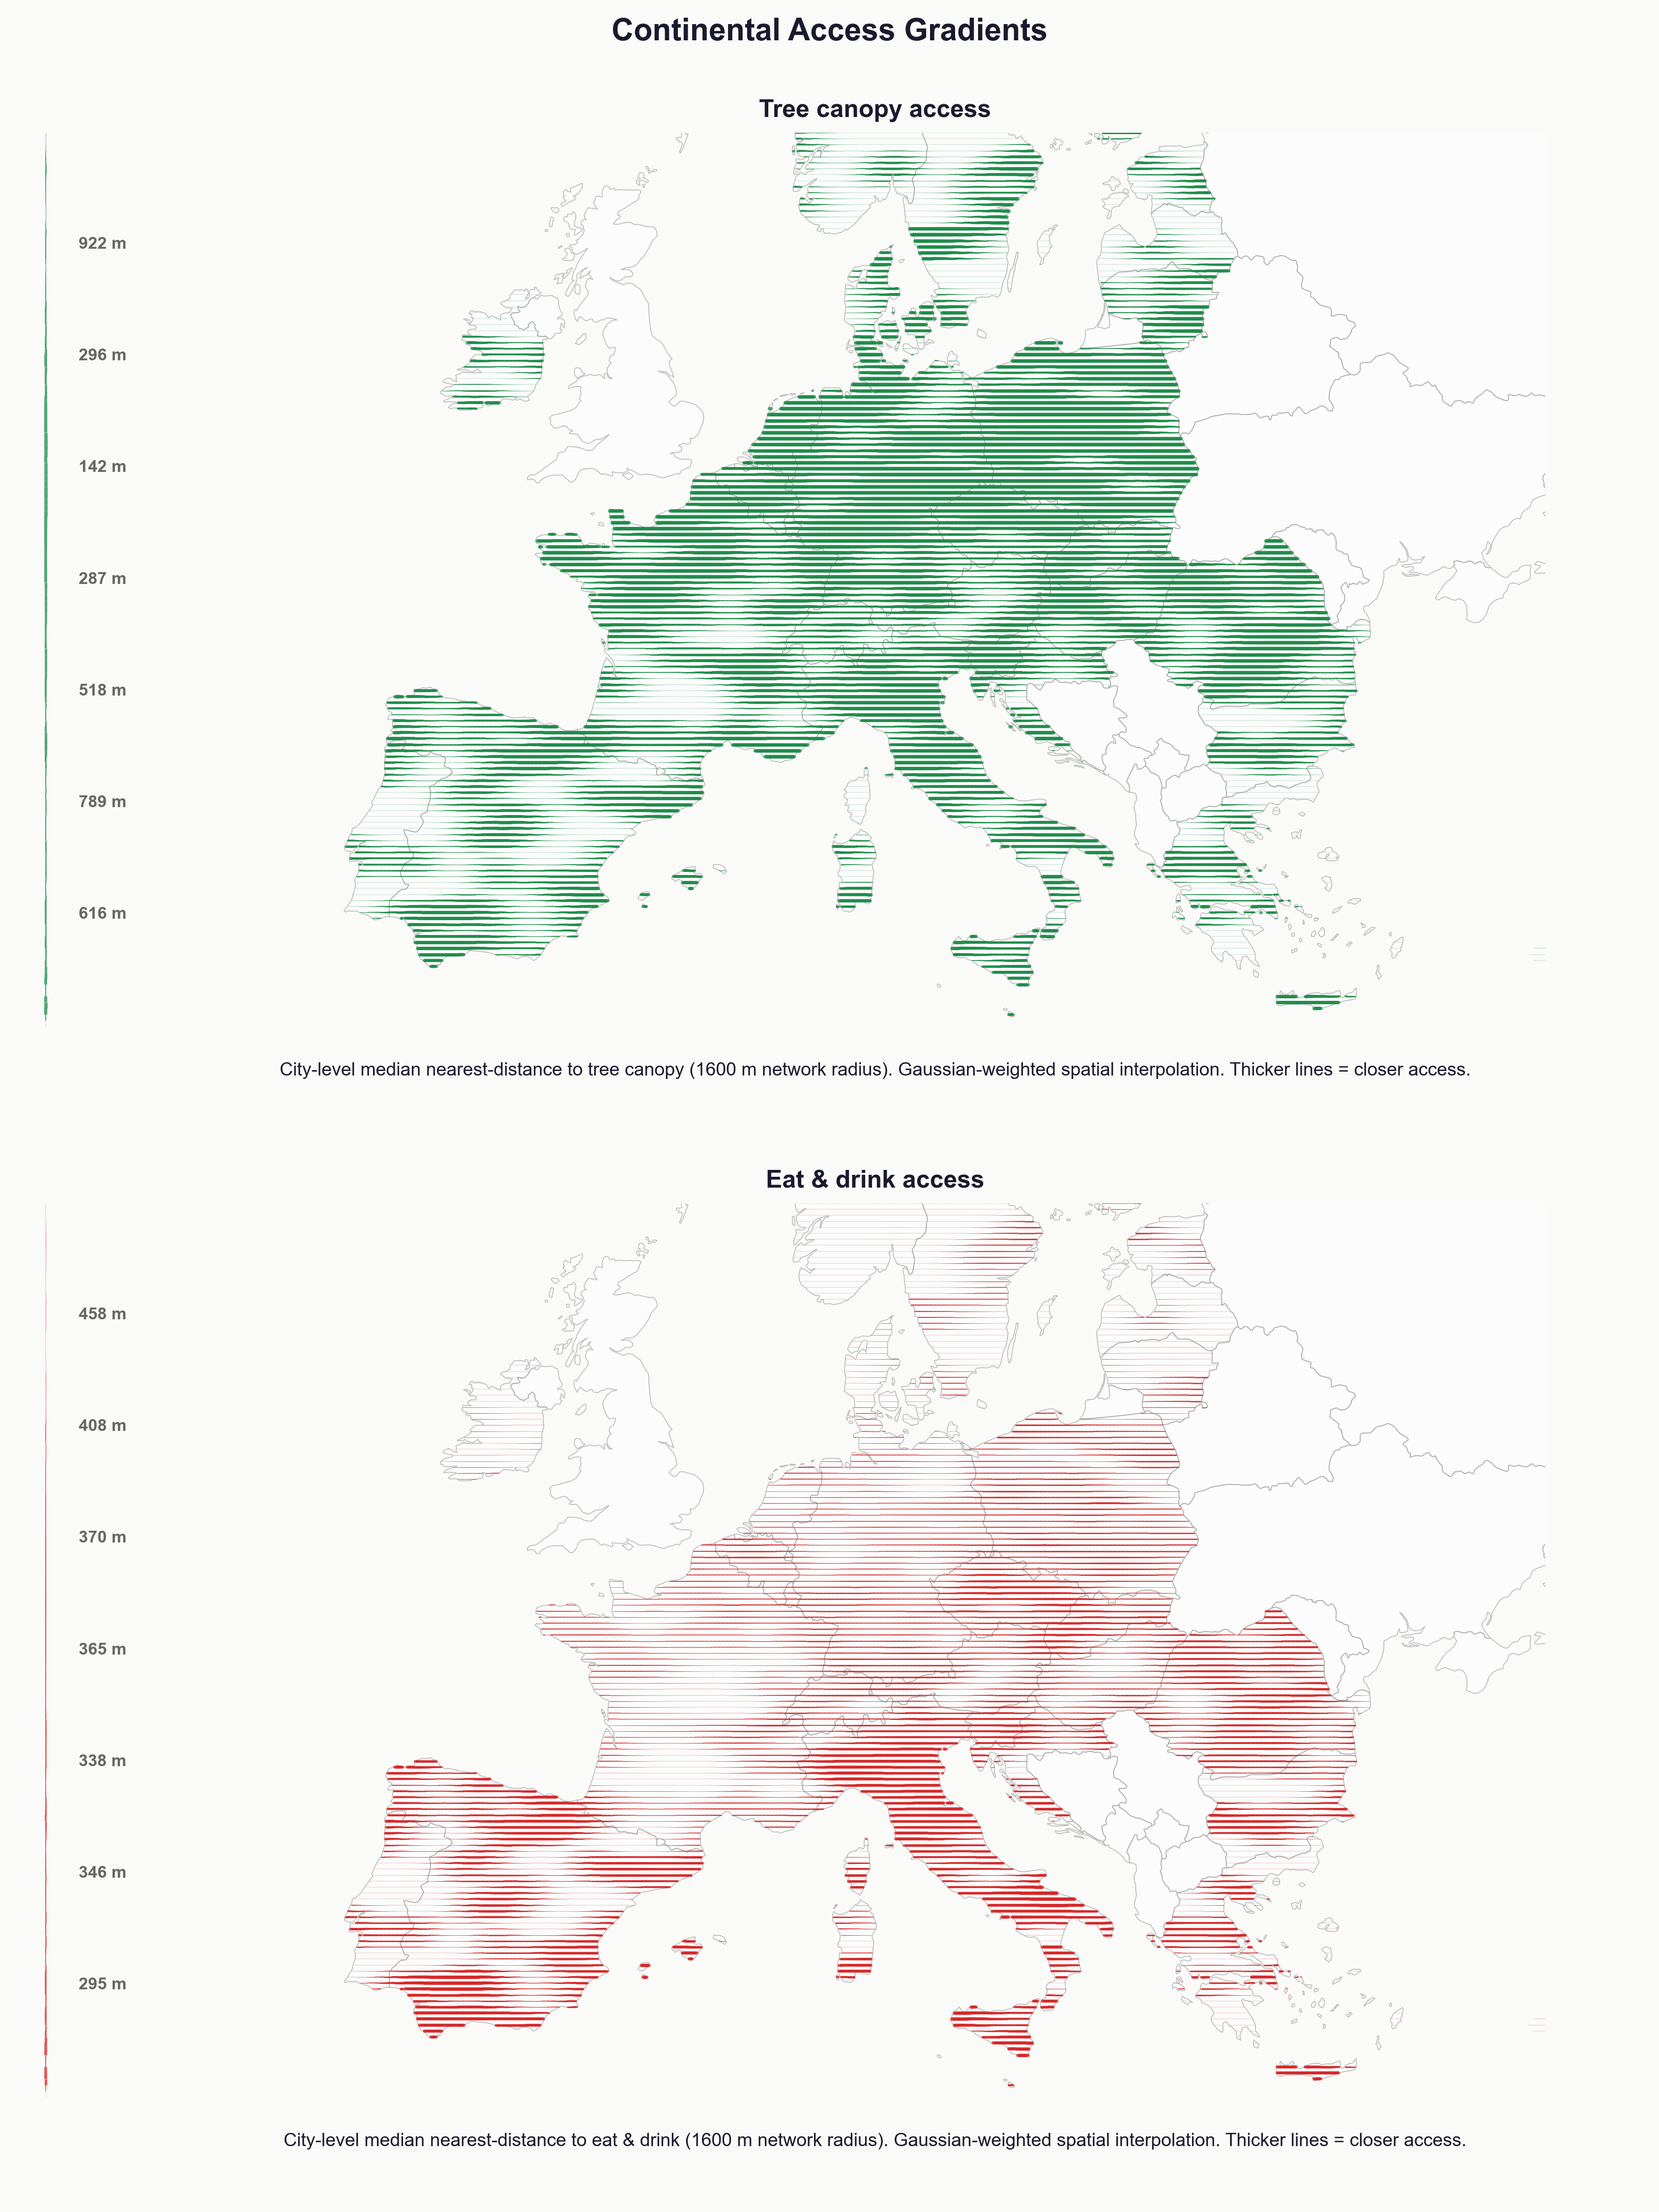
\includegraphics[width=0.98\textwidth]{outputs/atlas/plate9_scanlines.png}
  \caption{Continental scanline maps: tree-canopy proximity and eat \& drink proximity across \nCities{} cities.}
  \label{fig:plate9}
\end{figure}

These two plates situate the morphological patterns in geographic and institutional context. Plate~9 maps two continental gradients across all \nCities{} cities; Plate~10 presents four paired city comparisons in which different combinations of morphological and institutional dimensions vary.

Plate~9 (Figure~\ref{fig:plate9}) uses scanlines where the thickness encodes proximities based on adjacent cities. Tree-canopy proximity (measured as walking distance to the nearest Copernicus Street Tree Layer polygon, not to individual street trees) thickens across Scandinavia, the Baltic states, Poland, and Germany, where the cluster-median city is roughly \distTreesCoolMed\,m from mapped canopy. It thins across the Mediterranean, where the cluster-median city is around \distTreesWarmMed\,m. The gradient tracks climate but also planning tradition: Polish cities (whose socialist-era estates were laid out with systematic greenery and tree stands \citep{starczewski2024green}) and Nordic cities (which retained existing forest cover within suburban expansion \citep{hautamaki2022modern}) show shorter canopy distances than southern European cities. Eat-and-drink proximity reverses the pattern: the cluster-median city is around \distEatDrinkSouthMed\,m in Italy, Spain, and Greece, while in the Nordic countries it is closer to \distEatDrinkNorthMed\,m, a pattern consistent with food and drink establishments being more dispersed through residential fabric in Mediterranean cities than in Nordic ones.

\begin{figure}[htp]

  \centering
  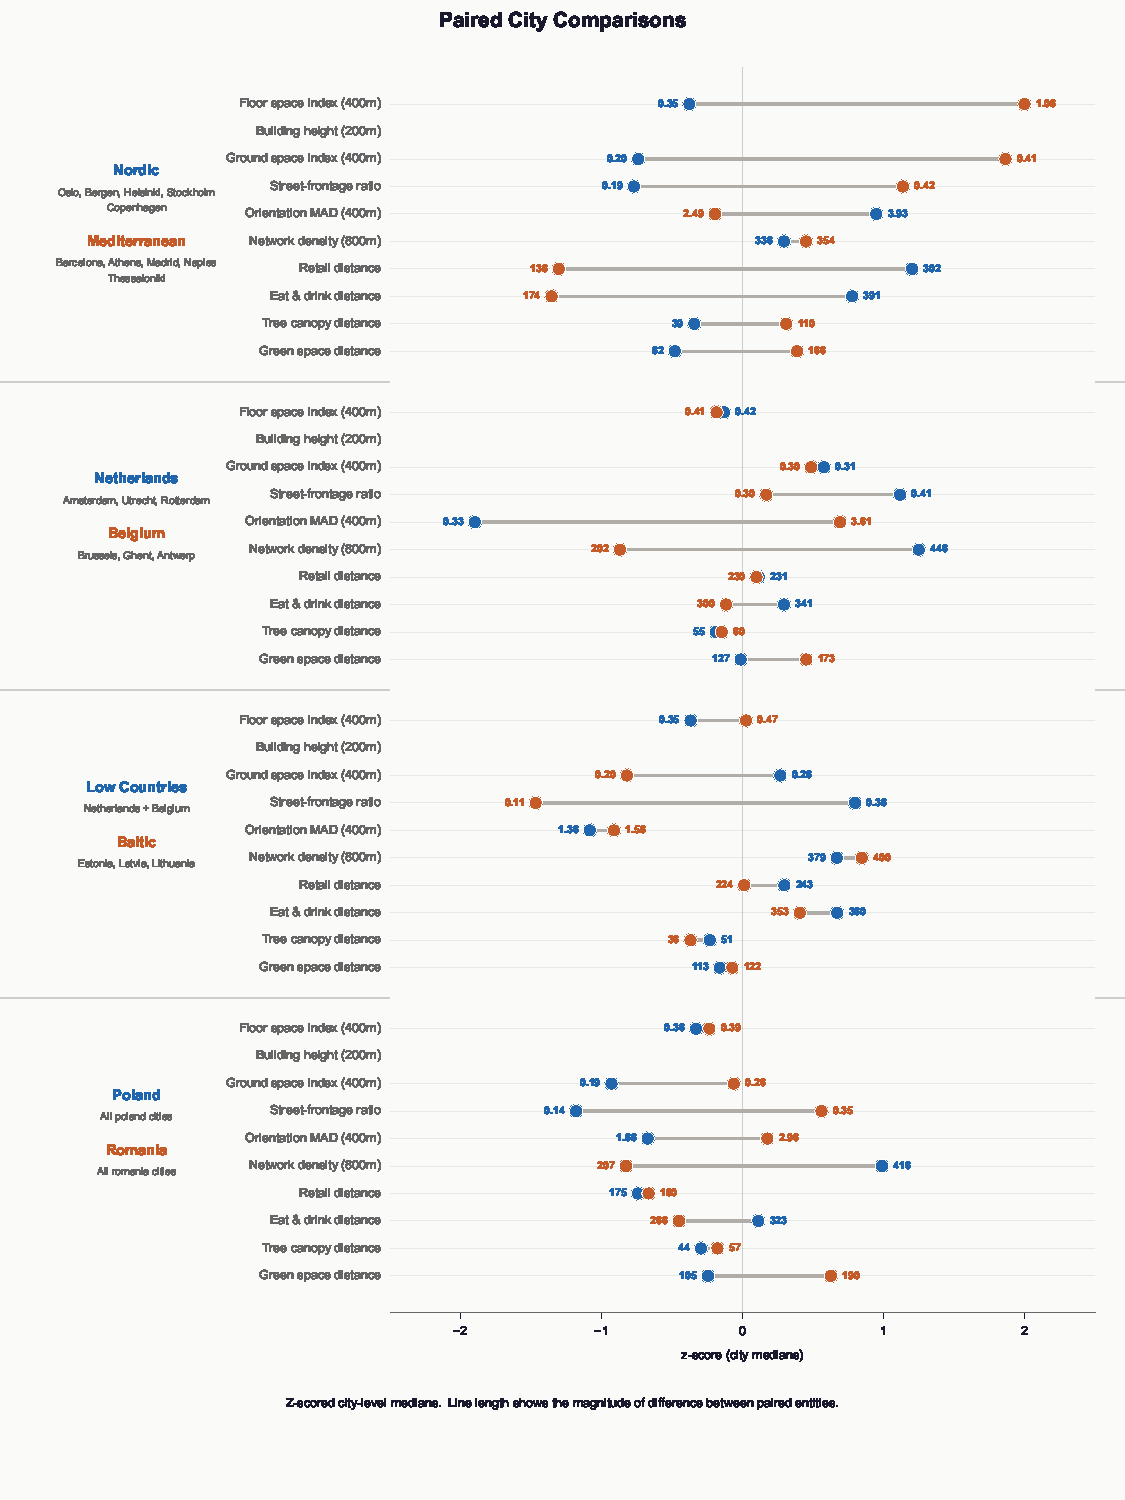
\includegraphics[width=0.98\textwidth]{outputs/atlas/plate10_comparisons.pdf}
  \caption{Four paired city comparisons across morphological and accessibility metrics.}
  \label{fig:plate10}
\end{figure}

The scanlines establish continental gradients but cannot explain them: the Nordic--Mediterranean contrast, for instance, bundles climate, building tradition, and commercial culture into a single spatial pattern. Plate~10 (Figure~\ref{fig:plate10}) uses four paired city comparisons, each varying a different combination of morphological and institutional dimensions.

\paragraph{Nordic vs Mediterranean}
The broadest contrast pairs five Nordic cities (Oslo, Bergen, Helsinki, Stockholm, Copenhagen) with five Mediterranean cities (Barcelona, Athens, Madrid, Naples, Thessaloniki). Building intensity, continuity, height, and irregularity all diverge together. Commercial service distances are shorter in the Mediterranean group (retail \compMedRetail\,m versus \compNordicRetail\,m), while tree-canopy distances run the opposite way.

\paragraph{Netherlands vs Belgium}
Amsterdam, Utrecht, and Rotterdam share a terraced row-house tradition with Brussels, Ghent, and Antwerp, giving both groups similar continuity. They diverge on irregularity and street-network density, yet retail distances remain broadly comparable (\compNLRetail\,m versus \compBERetail\,m).

\paragraph{Low Countries vs Baltic}
The Low Countries (Netherlands and Belgium) and the Baltic states (Estonia, Latvia, Lithuania) have comparable street-network densities but diverge on continuity and intensity, the Baltic states reaching higher FSI through freestanding blocks. Commercial and green-space distances are nonetheless similar (retail \compLCRetail\,m versus \compBalticRetail\,m; green \compLCGreen\,m versus \compBalticGreen\,m).

\paragraph{Poland vs Romania}
Both share a post-socialist inheritance but diverged on planning approach in the latter half of the twentieth century \citep{stanilov2007post, tsenkova2006urban}. Polish cities show higher street-network density while Romania's frontage ratio is higher, yet commercial distances are again similar (\compPLRetail\,m versus \compRORetail\,m) and green-space distances shorter in Poland (\compPLGreen\,m versus \compROGreen\,m).

Across the four comparisons, differences in Continuity and Intensity tend to accompany differences in commercial access distances. Irregularity does not: the pairs that diverge chiefly on layout order show near-identical commercial distances, and the within-city decomposition assigns the axis a negligible marginal share for commercial outcomes (\ref{sec:analytical-supplement}). We record this explicitly as a null result. The Irregularity axis discriminates planning traditions and development histories (Plates~2--3), but layout order carries no consistent commercial-access signal once intensity and continuity are accounted for.

% ==============================================================================
\section{Plates 11 \& 12 --- Density and Morphology}
\label{sec:plate11}
% ==============================================================================

\begin{figure}[htp]

  \centering
  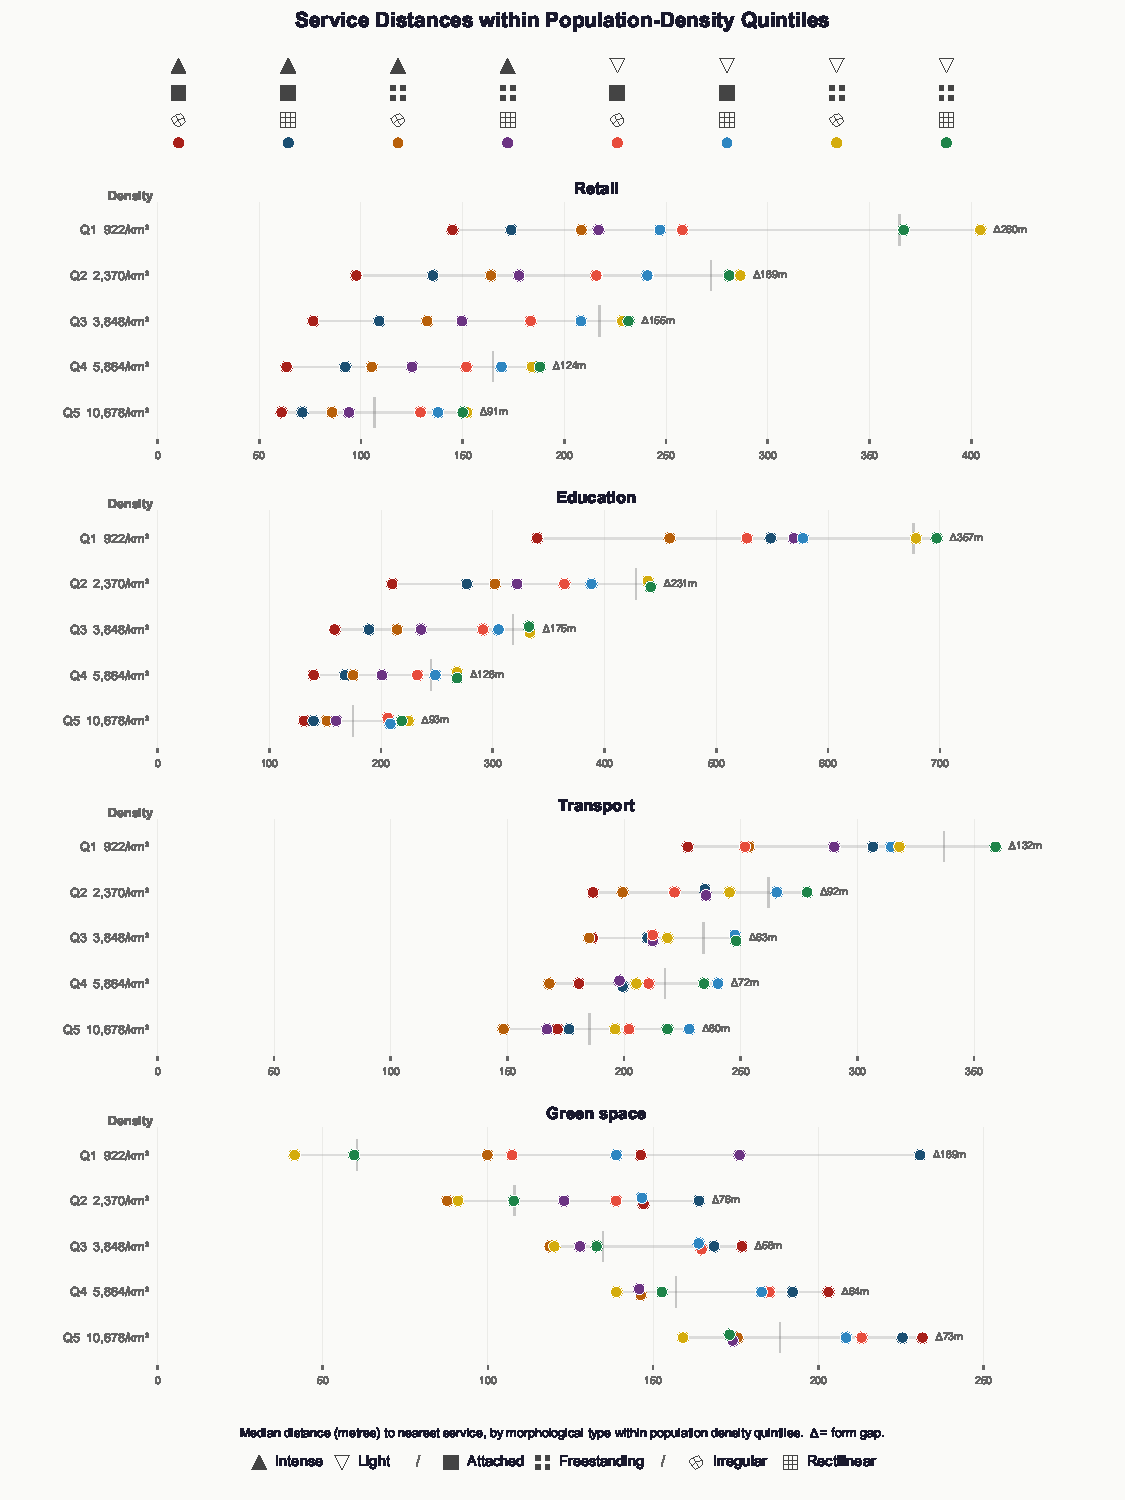
\includegraphics[width=0.98\textwidth]{outputs/atlas/plate11_density_form.pdf}
  \caption{Service distances by morphological type within population-density quintiles.}
  \label{fig:plate11}
\end{figure}

These two plates relate access to density and to form. Plate~11 bins all classified streets into population-density quintiles and compares the eight morphological types within each band; Plate~12 maps street-level access across the intensity--continuity form space. Within-city matched-pair comparisons are provided in the analytical supplement (\ref{sec:analytical-supplement}).

Within each density quintile (Figure~\ref{fig:plate11}) the morphological types remain distinct, and the spread is widest in the sparsest band: at Q1 (median $\sim$\num{\dqMedianOne}/km$^2$) the retail gap between the most and least accessible types is \dqRetailQOnegap\,m, with education wider still at \dqEducationQOnegap\,m, narrowing to \dqRetailQThreegap\,m of retail at Q3 (\dqRetailQThreegapPct\% of the continental median) and \dqRetailQFivegap\,m at Q5. Green space shows the reverse, its type gap largest at Q1 (\dqGreenQOnegap\,m) and smaller in every later band, so the inversion of Plates~5--7 is most pronounced in sparse fabric. Because the quintiles pool streets across cities and countries, these differences reflect both morphological variation and city-level factors (POI coverage, planning context, economic structure) that co-vary with type.

\begin{figure}[htp]
  \centering
  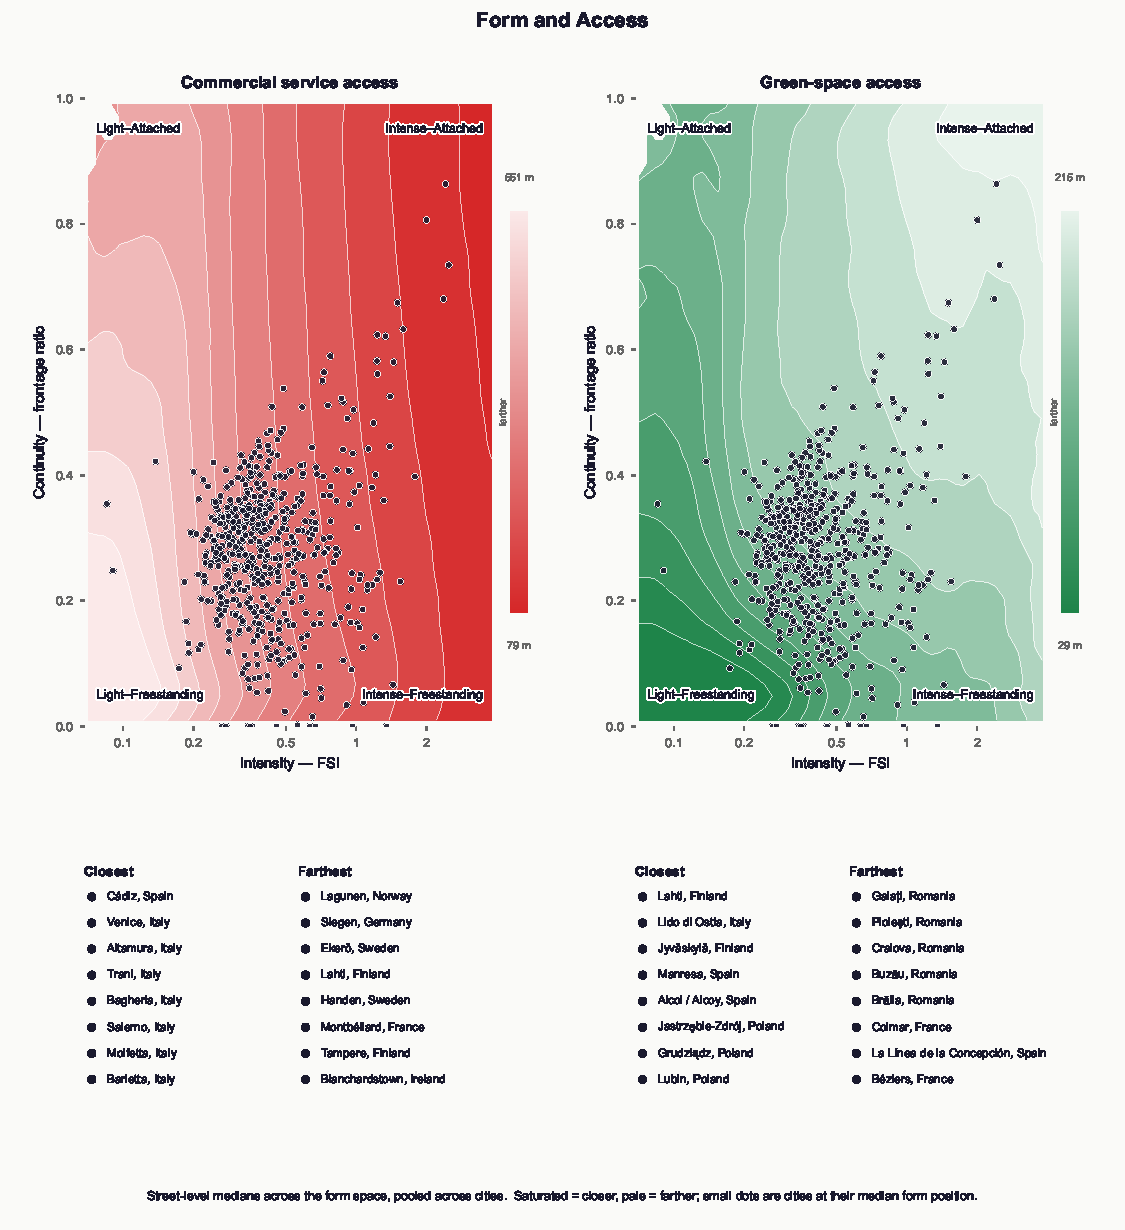
\includegraphics[width=\textwidth]{outputs/atlas/plate12_formspace.pdf}
  \caption{Walking distance to commercial services (left) and green space (right) across the intensity--continuity morphological form space. Each cell is shaded by the street-level median distance of the streets it contains, red for commercial and green for green space, with more saturated tones indicating shorter distances and paler tones longer ones; small dots mark cities at their median form-space position. The two panels use independent colour scales, and green-space distances span a substantially smaller range than commercial. The closest and farthest cities on each measure are listed beneath.}
  \label{fig:plate12}
\end{figure}

Plate~12 (Figure~\ref{fig:plate12}) maps access onto the two morphological axes, intensity (FSI) and continuity (frontage ratio), shading each cell by the median walking distance of its streets for commercial services (left, a composite of retail, health \& medical, education, eat \& drink, and business \& services) and green space (right). The two surfaces run in opposite directions: commercial distance falls along the intensity axis in a broadly vertical gradient, continuity a secondary influence, whereas green-space distance inverts and runs diagonally, shortest in the Light--Freestanding corner (low intensity and low continuity) and longest in dense, attached fabric, where continuity contributes more than it does for commercial access. The form space thus shows directly the green inversion of Plates~5--7 and the differing roles of intensity and continuity reported in the appendix (Table~\ref{tab:marginal}).

Because city medians compress the street-level range, the city dots cluster towards the lower-intensity centre rather than the extremes, and the form--access gradients soften at the city scale. Some compact cities nonetheless achieve short green-space distances, for example in Poland, Spain, and Italy, so compactness and green-space access are not inherently in tension (cf.\ \ref{sec:analytical-supplement}).

The two gradients differ in direction, and the difference has practical consequences. Commercial access improves along the intensity axis, the dimension that regulation controls through permitted floor area; green access depends more on continuity, and because the green gradient spans a smaller range, targeted provision can offset what intensification would otherwise cost. The form space also serves as a diagnostic frame: any street or city can be located in it from two measurements, and its expected commercial and green distances read off from the surrounding cells, giving planners a direct way to position a district against \nCities{}-city norms.

% ==============================================================================
\section{Discussion}
\label{sec:discussion}
% ==============================================================================

\subsection{Form and access}

One of the more consistent patterns in the atlas is that morphological type is associated with pedestrian access to commercial services even when streets are compared within the same city and population-density band. Intense--Attached types show the shortest walking distances and the widest mix of categories; Light--Freestanding types show the longest distances and the highest rates of service absence. The gap between types at the middle population-density quintile amounts to \dqRetailQThreegapPct\% of the continental median and narrows steadily towards the densest band. A within-city decomposition (\ref{sec:analytical-supplement}) finds that the three morphological axes account for \rSqMorphMin--\rSqMorphMax\% of within-city variance in commercial service distances, while adding population density at census resolution adds little, though this may partly reflect the resolution mismatch between 1\,km$^2$ census grids and the \kernelDist\,m morphological kernel. The mismatch bounds the claim. The census grid cannot resolve density variation between neighbouring streets, but it does fix the neighbourhood-scale density at which the matched comparisons are made, so the defensible reading is that built form discriminates commercial access at any given neighbourhood-scale density observable in pan-European data. A finer population grid could reveal street-scale density effects within neighbourhoods; it could not remove the form gradient documented across them. FSI is itself a fine-grained measure of built (as opposed to residential) density, so the comparison separates built form from residential crowding; it does not claim that density in general is irrelevant. These observations are consistent with the Spacematrix argument that building density is a multi-indicator condition whose components carry independent information \citep{berghauser2010spacematrix, godoyshimizu2021density}.

Within the morphological signal, Intensity and Continuity appear to operate on different service domains. For commercial services, FSI accounts for the larger share of the within-city association (\mFSIshareMin--\mFSIshareMax\%), with frontage adding \mContshareMin--\mContshareMax\% independently. A plausible mechanism for the frontage contribution runs through the ground floor: FSI concentrates potential customers and floor space around a street, while continuous frontage supplies the street-facing ground-floor premises that small commercial establishments occupy. This would explain why the frontage effect is clearest for retail, the category most dependent on ground-floor premises and passing footfall (Plates~5--6), and why continuity cuts commercial desert fractions by a third to a half at constant intensity (Plate~6). The dataset does not observe ground-floor use directly, so this reading remains inferential. For green space the pattern inverts: frontage ratio carries the larger share (\mContGreenShare\%) and FSI only \mFSIGreenShare\%. Because the inverted green gradient is shallower than the commercial one, the green-space gap between compact and dispersed fabric is smaller than the corresponding commercial gap. At the city level the two access dimensions do not trade off as simply: Spain, Italy, and Poland each have cities with short distances on both commercial and green dimensions, while German and Nordic cities tend towards short green distances alongside longer commercial ones.

Network structure is correlated with morphological type (fine-grained perimeter-block fabric tends to produce denser street networks), and network centrality alone accounts for \mNetworkRsqMin--\mNetworkRsqMax\% of within-city variance in commercial service distances. Part of the association attributed to building arrangement may therefore run through network structure, which the dataset's morphological and network metrics together could help disentangle. Form is also entangled with the commercial cultures and development histories that accompany it: Intense--Attached fabric tends to coincide with histories of mixed-use intensification and dispersed small-establishment commercial activity. Separating the two is a promising direction for further research, for which the cross-sectional patterns documented here offer a starting point.

\subsection{Regional and institutional patterns}

The atlas records a broad periodisation that cuts across European regions. Pre-mid-twentieth-century development tends to correspond to Intense--Attached types; mid-twentieth-century expansion (modernist reconstruction, mikrorayon planning, suburban growth) produced the sparser, more detached fabric that now forms the majority of the network. The paired comparisons in Plate~10 show how distinct planning traditions register on these axes while often producing similar commercial outcomes. The recurrence of such patterns across \nCities{} cities in different national contexts is a starting point for more targeted studies of how planning traditions and regulatory codes shape pedestrian access \citep{talen2012city}.

\subsection{Applications and planning debates}

Beyond description, the classification serves three uses. First, it provides comparative research with a common language, since a type label computed identically everywhere replaces ad hoc descriptors of fabric. Second, it supports monitoring: as sources refresh, a district's movement in the classification space records densification, infill, or estate regeneration in commensurable terms. Third, it offers design and policy a target vocabulary, since the paired-city and matched-density results indicate which axis (mass, enclosure, or order) is associated with the outcome a plan seeks.

The patterns documented here also bear on several active debates. Proposals for the 15-minute city presuppose that everyday services can be reached on foot \citep{moreno2021fifteen}; the atlas measures how far each European street currently is from that condition and shows the shortfall to be structured by fabric type, with the condition largely met in Intense--Attached streets while deserts exceed 40\% for several everyday categories in the Light--Freestanding fabric that carries the majority of streets. Debates on the compact city have long weighed access gains against amenity and green-space costs \citep{neuman2005compact}; the green inversion documented in Plates~5--7 and~12 supports a more specific position, since the trade-off is real at street level but weakens across cities, and compact cities with short green distances exist in several countries. For transit-oriented development, whose design dimension is often reduced to density and diversity measures \citep{cervero1997travel}, the frontage results identify street-level continuity as a distinct, measurable design variable carrying an access signal independent of built mass. And for the healthy-cities agenda, which calls for comparable pedestrian-scale indicators across jurisdictions \citep{gilescorti2016city}, the dataset supplies that measurement layer for \nCities{} cities under a single method.

\subsection{Demographic patterns}

The demographic gradient parallels the access pattern: the Light types that carry the longest walks also host the higher shares of children (Plate~8), with education distances the widest of all and exceeding the retail gap at every density quintile (Plate~11). The mechanisms proposed in Section~\ref{sec:plate8} are distinguishable in principle: a housing-supply explanation implies the gradient should track dwelling size and cost data, life-cycle sorting implies it should attenuate in cities where family-sized dwellings exist in Intense fabric, and provider-location logic implies education distances should respond to purchasing density rather than to child share. Each is testable within the dataset by pairing the demographic interpolations with the access metrics city by city, and this juxtaposition is among the more policy-relevant questions the atlas raises.

\subsection{Limitations}

Several limitations condition how the patterns in the atlas are interpreted. The three-axis classification reduces a continuous morphological space to eight discrete types, and within-type variation is substantial (Plate~7): a type label describes a central tendency rather than a reliable prediction for any individual street, and streets near a threshold boundary are more likely to be misclassified. The atlas also captures a single snapshot of each source (vintages documented in the companion data paper \citep{simons2024soar}) and cannot track change over time.

On the data side, Overture Maps POI coverage is uneven across countries. A companion study shows fair, category-dependent agreement with official registries in France and the Netherlands \citep{simons2024soar}, but coverage in eastern and southern Europe may be less complete, which would inflate measured accessibility distances. Because coverage gaps and morphological type are spatially correlated, data completeness may contribute to the observed form--access patterns. Green-space proximity is measured against Urban Atlas polygons with a minimum mapping unit of approximately 0.25 hectares, so small pocket parks and courtyards are not captured; this may overstate green-space distances in Intense fabric, which tends to rely on smaller interventions. Building heights come from the 2012 Copernicus Digital Height Model and do not reflect recent construction. Finally, nearest-distance captures proximity to the closest facility rather than the range of choice available within walking distance.

% ==============================================================================
\section{Conclusion}
\label{sec:conclusion}
% ==============================================================================

This atlas has measured \nTotalM{} million European streets and organised the \nClassifiedM{} million with complete morphological data into eight types defined by three measurable axes (intensity, continuity, and irregularity), showing that this form is systematically associated with pedestrian access to services and green space, and with demographic composition, across \nCities{} cities. It is, to our knowledge, the first account of European urban fabric at pedestrian scale to span the continent with uniform methods. The Intense--Attached types combine building mass with continuous facade enclosure, ground-floor frontage, and short walks to commercial services; they account for approximately \pctIntenseAttached\% of the continent's classified streets.

The central regularity is that morphological type tracks pedestrian access to commercial services even within the same city and population-density band: at matched density the Attached--Freestanding gap is \matchedGainMin--\matchedGainMax\,m across the four matched service categories, holding in \matchedDirMin--\matchedDirMax\% of cities, so the signal follows form rather than density within the limits of the 1\,km census grid. The types recur across national borders in patterns shaped by planning tradition and topographic constraint, and the Light types that carry the longest service distances also host the higher shares of children. Green-space access, by contrast, is not determined by form alone: the street-level compact--green trade-off weakens across cities, with some compact cities (Poland, Spain, Italy) close to both commercial and green dimensions, suggesting green provision can be addressed by planning policy.

The SOAR-EU dataset and its adjustable thresholds are openly available, supporting temporal monitoring as sources refresh, within-city analyses of the regulatory variation the atlas documents, quasi-experimental designs around historical disruptions, and extension to dimensions these plates do not address. More broadly, the atlas is offered as empirical infrastructure for comparative urban morphology: a shared measurement base and descriptive vocabulary under which \nCities{} cities can be studied with the same instruments. Questions that have so far been confined to single cities or small samples, such as how planning regimes shape pedestrian access, how fabric conditions demographic sorting, and how green provision responds to compactness, can now be addressed at the scale of a continent.

% ==============================================================================
% Declarations
% ==============================================================================

\section*{Declaration of Competing Interest}

The authors declare that they have no known competing financial interests or personal relationships that could have appeared to influence the work reported in this paper.

\section*{Ethics Statement}

This research did not involve human subjects, animal experiments, or data collected from social media platforms. Census demographics are aggregated to 1\,km$^2$ grid cells and contain no individual-level information. All source datasets are publicly accessible under their respective licences.

\section*{Declaration of Generative AI and AI-assisted Technologies in the Writing Process}

The original data processing was undertaken with minimal AI-assistive technologies. The manuscript itself, together with manuscript-related code and figures, was completed with the aid of Claude (Anthropic). After using this tool, the authors reviewed and edited the content as needed and take full responsibility for the content of the publication.

\section*{CRediT Author Statement}

\noindent\textbf{Gareth Simons}: Conceptualisation, Methodology, Software, Data curation, Formal analysis, Visualisation, Writing --- original draft.\\
\textbf{Kayvan Karimi}: Conceptualisation, Supervision, Review.\\
\textbf{Sepehr Zhand}: Conceptualisation, Review.

\section*{Acknowledgements}

This project has received funding from the European Union's Horizon Europe Research and Innovation Programme under Grant Agreement No.\ 101078890, and from UK Research and Innovation (UKRI) under the UK government's Horizon Europe funding guarantee under grant numbers 10052856 and 10050784.

\section*{Data and Code Availability}

The SOAR-EU dataset is available at Zenodo (\href{https://doi.org/10.5281/zenodo.18961227}{10.5281/zenodo.18961227}), licensed under the Open Database License (ODbL~1.0). The dataset, input-data provenance, processing pipeline, and per-metric validation are documented in the companion data paper \citep{simons2024soar}. Analysis and figure-generation code for the present paper is available at \href{https://github.com/UCL/t2e-soar-eu}{github.com/UCL/t2e-soar-eu} (AGPL-3.0), including the classification implementation, the plate-generation scripts, the within-city decomposition and matched-pair analyses reported in \ref{sec:analytical-supplement}, and the macro-generation utilities that populate the numerical values in the text.

% ==============================================================================
% References
% ==============================================================================

\bibliographystyle{elsarticle-harv}
% \bibliography{references}

\begin{thebibliography}{45}

  \bibitem[Angel et al.(2016)]{angel2016atlas}
  Angel, S., Blei, A.M., Parent, J., Lamson-Hall, P., Galarza S\'{a}nchez, N., 2016.
  \newblock \emph{Atlas of Urban Expansion --- 2016 Edition}.
  \newblock NYU Urban Expansion Program, UN-Habitat, and Lincoln Institute of Land Policy, New York.

  \bibitem[Araldi and Fusco(2019)]{araldi2019street}
  Araldi, A., Fusco, G., 2019.
  \newblock From the street to the metropolitan region: Pedestrian perspective in urban fabric analysis.
  \newblock \emph{Environment and Planning B: Urban Analytics and City Science} 46(7), 1243--1263.
  \newblock \url{https://doi.org/10.1177/2399808319832612}.

  \bibitem[Ballantyne and Berragan(2024)]{ballantyne2024overture}
  Ballantyne, P., Berragan, C., 2024.
  \newblock Overture Point of Interest data for the United Kingdom: A comprehensive, queryable open data product, validated against Geolytix supermarket data.
  \newblock \emph{Environment and Planning B: Urban Analytics and City Science} 51(8), 1974--1980.
  \newblock \url{https://doi.org/10.1177/23998083241263124}.

  \bibitem[Barrington-Leigh and Millard-Ball(2017)]{barringtonleigh2017world}
  Barrington-Leigh, C., Millard-Ball, A., 2017.
  \newblock The world's user-generated road map is more than 80\% complete.
  \newblock \emph{PLoS ONE} 12(8), e0180698.
  \newblock \url{https://doi.org/10.1371/journal.pone.0180698}.

  \bibitem[Berghauser~Pont and Haupt(2010)]{berghauser2010spacematrix}
  Berghauser~Pont, M., Haupt, P., 2010.
  \newblock \emph{Spacematrix: Space, Density and Urban Form}.
  \newblock NAi Publishers, Rotterdam.

  \bibitem[Berghauser~Pont et al.(2019)]{berghauser2019systematic}
  Berghauser~Pont, M., Stavroulaki, G., Bobkova, E., Gil, J., Marcus, L., Olsson, J., Sun, K., Serra, M., Hausleitner, B., Dhanani, A., Legeby, A., 2019.
  \newblock The spatial distribution and frequency of street, plot and building types across five European cities.
  \newblock \emph{Environment and Planning B: Urban Analytics and City Science} 46(7), 1226--1242.
  \newblock \url{https://doi.org/10.1177/2399808319857450}.

  \bibitem[Boeing(2019)]{boeing2019urban}
  Boeing, G., 2019.
  \newblock Urban spatial order: street network orientation, configuration, and entropy.
  \newblock \emph{Applied Network Science} 4, 67.
  \newblock \url{https://doi.org/10.1007/s41109-019-0189-1}.

  \bibitem[Boeing(2020)]{boeing2020multi}
  Boeing, G., 2020.
  \newblock A multi-scale analysis of 27,000 urban street networks: Every US city, town, urbanized area, and Zillow neighborhood.
  \newblock \emph{Environment and Planning B: Urban Analytics and City Science} 47(4), 590--608.
  \newblock \url{https://doi.org/10.1177/2399808318784595}.

  \bibitem[Busquets(2005)]{busquets2005barcelona}
  Busquets, J., 2005.
  \newblock \emph{Barcelona: The Urban Evolution of a Compact City}.
  \newblock Nicolodi / Harvard University Graduate School of Design, Rovereto.

  \bibitem[Caniggia and Maffei(2001)]{caniggia2001architectural}
  Caniggia, G., Maffei, G.L., 2001.
  \newblock \emph{Architectural Composition and Building Typology: Interpreting Basic Building}.
  \newblock Alinea, Florence.

  \bibitem[Cervero and Kockelman(1997)]{cervero1997travel}
  Cervero, R., Kockelman, K., 1997.
  \newblock Travel demand and the 3Ds: Density, diversity, and design.
  \newblock \emph{Transportation Research Part D: Transport and Environment} 2(3), 199--219.
  \newblock \url{https://doi.org/10.1016/S1361-9209(97)00009-6}.

  \bibitem[De~Decker(2008)]{dedecker2008facets}
  De~Decker, P., 2008.
  \newblock Facets of housing and housing policies in Belgium.
  \newblock \emph{Journal of Housing and the Built Environment} 23(3), 155--171.
  \newblock \url{https://doi.org/10.1007/s10901-008-9110-4}.

  \bibitem[Dibble et al.(2019)]{dibble2019origin}
  Dibble, J., Prelorendjos, A., Romice, O., Zanella, M., Strano, E., Pagel, M., Porta, S., 2019.
  \newblock On the origin of spaces: Morphometric foundations of urban form evolution.
  \newblock \emph{Environment and Planning B: Urban Analytics and City Science} 46(4), 707--730.
  \newblock \url{https://doi.org/10.1177/2399808317725075}.

  \bibitem[Diefendorf(1993)]{diefendorf1993wake}
  Diefendorf, J.M., 1993.
  \newblock \emph{In the Wake of War: The Reconstruction of German Cities after World War II}.
  \newblock Oxford University Press, New York.

  \bibitem[Dovey and Pafka(2014)]{dovey2014urban}
  Dovey, K., Pafka, E., 2014.
  \newblock The urban density assemblage: Modelling multiple measures.
  \newblock \emph{Urban Design International} 19, 66--76.
  \newblock \url{https://doi.org/10.1057/udi.2013.13}.

  \bibitem[{European Commission}(2024)]{florczyk2019ghs}
  European Commission, Joint Research Centre, 2024.
  \newblock GHS Urban Centre Database R2024A [dataset].
  \newblock \url{https://human-settlement.emergency.copernicus.eu/ghs_ucdb_2024.php}.

  \bibitem[Faludi and van~der~Valk(1994)]{faludi1994rule}
  Faludi, A., van~der~Valk, A.J., 1994.
  \newblock \emph{Rule and Order: Dutch Planning Doctrine in the Twentieth Century}.
  \newblock Kluwer Academic Publishers, Dordrecht.

  \bibitem[Fleischmann et al.(2022)]{fleischmann2022morphological}
  Fleischmann, M., Feliciotti, A., Romice, O., Porta, S., 2022.
  \newblock Methodological foundation of a numerical taxonomy of urban form.
  \newblock \emph{Environment and Planning B: Urban Analytics and City Science} 49, 1283--1299.
  \newblock \url{https://doi.org/10.1177/23998083211059835}.

  \bibitem[Giles-Corti et al.(2016)]{gilescorti2016city}
  Giles-Corti, B., Vernez-Moudon, A., Reis, R., Turrell, G., Dannenberg, A.L., Badland, H., Foster, S., Lowe, M., Sallis, J.F., Stevenson, M., Owen, N., 2016.
  \newblock City planning and population health: a global challenge.
  \newblock \emph{The Lancet} 388(10062), 2912--2924.
  \newblock \url{https://doi.org/10.1016/S0140-6736(16)30066-6}.

  \bibitem[Godoy-Shimizu et al.(2021)]{godoyshimizu2021density}
  Godoy-Shimizu, D., Steadman, P., Evans, S., 2021.
  \newblock Density and morphology: from the building scale to the city scale.
  \newblock \emph{Buildings and Cities} 2(1), 92--113.
  \newblock \url{https://doi.org/10.5334/bc.83}.

  \bibitem[Hamaina et al.(2012)]{hamaina2012towards}
  Hamaina, R., Leduc, T., Moreau, G., 2012.
  \newblock Towards urban fabrics characterization based on buildings footprints.
  \newblock In: Gensel, J., Josselin, D., Vandenbroucke, D. (Eds.), \emph{Bridging the Geographic Information Sciences}. Springer, Berlin, pp.~327--346.
  \newblock \url{https://doi.org/10.1007/978-3-642-29063-3_18}.

  \bibitem[Hautam\"aki and Donner(2022)]{hautamaki2022modern}
  Hautam\"aki, R., Donner, J., 2022.
  \newblock Modern living in a forest --- landscape architecture of Finnish forest suburbs in the 1940s--1960s.
  \newblock \emph{Geografiska Annaler: Series B, Human Geography} 104(3), 250--268.
  \newblock \url{https://doi.org/10.1080/04353684.2021.1989320}.

  \bibitem[Herfort et al.(2023)]{herfort2023spatio}
  Herfort, B., Lautenbach, S., Porto de Albuquerque, J., Anderson, J., Zipf, A., 2023.
  \newblock A spatio-temporal analysis investigating completeness and inequalities of global urban building data in OpenStreetMap.
  \newblock \emph{Nature Communications} 14, 3985.

  \bibitem[Kropf(2009)]{kropf2009aspects}
  Kropf, K., 2009.
  \newblock Aspects of urban form.
  \newblock \emph{Urban Morphology} 13(2), 105--120.

  \bibitem[Louf and Barthelemy(2014)]{louf2014typology}
  Louf, R., Barthelemy, M., 2014.
  \newblock A typology of street patterns.
  \newblock \emph{Journal of the Royal Society Interface} 11, 20140924.
  \newblock \url{https://doi.org/10.1098/rsif.2014.0924}.

  \bibitem[Maloutas(2003)]{maloutas2003promoting}
  Maloutas, T., 2003.
  \newblock Promoting social sustainability: the case of Athens.
  \newblock \emph{City} 7(2), 167--181.
  \newblock \url{https://doi.org/10.1080/1360481032000136732}.

  \bibitem[Moreno et al.(2021)]{moreno2021fifteen}
  Moreno, C., Allam, Z., Chabaud, D., Gall, C., Pratlong, F., 2021.
  \newblock Introducing the ``15-minute city'': Sustainability, resilience and place identity in future post-pandemic cities.
  \newblock \emph{Smart Cities} 4(1), 93--111.
  \newblock \url{https://doi.org/10.3390/smartcities4010006}.

  \bibitem[Moudon(1997)]{moudon1997urban}
  Moudon, A.V., 1997.
  \newblock Urban morphology as an emerging interdisciplinary field.
  \newblock \emph{Urban Morphology} 1(1), 3--10.

  \bibitem[Neuman(2005)]{neuman2005compact}
  Neuman, M., 2005.
  \newblock The compact city fallacy.
  \newblock \emph{Journal of Planning Education and Research} 25(1), 11--26.
  \newblock \url{https://doi.org/10.1177/0739456X04270466}.

  \bibitem[Oliveira(2016)]{oliveira2016urban}
  Oliveira, V., 2016.
  \newblock \emph{Urban Morphology: An Introduction to the Study of the Physical Form of Cities}.
  \newblock Springer, Cham.

  \bibitem[{Overture Maps Foundation}(2026)]{overture2026}
  {Overture Maps Foundation}, 2026.
  \newblock Overture Maps Data --- Release 2026-05-20.0 [dataset].
  \newblock \url{https://docs.overturemaps.org/blog/2026/05/20/release-notes/}.

  \bibitem[Panerai et al.(2004)]{panerai2004urban}
  Panerai, P., Castex, J., Depaule, J.-C., Samuels, I., 2004.
  \newblock \emph{Urban Forms: The Death and Life of the Urban Block}.
  \newblock Architectural Press, Oxford.

  \bibitem[Simons(2021)]{simons2021thesis}
  Simons, G.D., 2021.
  \newblock \emph{Detection and prediction of urban archetypes at the pedestrian scale: computational toolsets, morphological metrics, and machine learning methods}.
  \newblock Ph.D. thesis, UCL (University College London).
  \newblock \url{https://discovery.ucl.ac.uk/id/eprint/10134012/}.

  \bibitem[Simons(2023)]{simons2023cityseer}
  Simons, G., 2023.
  \newblock The cityseer Python package for pedestrian-scale network-based urban analysis.
  \newblock \emph{Environment and Planning B: Urban Analytics and City Science} 50(5), 1328--1344.
  \newblock \url{https://doi.org/10.1177/23998083221133827}.

  \bibitem[Simons et al.(2026)]{simons2024soar}
  Simons, G., Karimi, K., Zhand, S., 2026.
  \newblock SOAR-EU: A Scalable, Open, Automatable, and Reproducible European Urban Dataset.
  \newblock Submitted to \emph{Scientific Data}.

  \bibitem[Stanilov(2007)]{stanilov2007post}
  Stanilov, K. (Ed.), 2007.
  \newblock \emph{The Post-Socialist City: Urban Form and Space Transformations in Central and Eastern Europe after Socialism}.
  \newblock Springer, Dordrecht.

  \bibitem[Starczewski et al.(2024)]{starczewski2024green}
  Starczewski, T., Rogatka, K., Noszczyk, T., Kukulska-Kozie\l{}, A., Cegielska, K., 2024.
  \newblock Green spaces in Polish large prefabricated housing estates developed in the socialist era.
  \newblock \emph{Journal of Housing and the Built Environment} 39(4), 1987--2007.
  \newblock \url{https://doi.org/10.1007/s10901-024-10147-0}.

  \bibitem[Talen(2012)]{talen2012city}
  Talen, E., 2012.
  \newblock \emph{City Rules: How Regulations Affect Urban Form}.
  \newblock Island Press, Washington, DC.

  \bibitem[Tsenkova and Nedovi\'{c}-Budi\'{c}(2006)]{tsenkova2006urban}
  Tsenkova, S., Nedovi\'{c}-Budi\'{c}, Z. (Eds.), 2006.
  \newblock \emph{The Urban Mosaic of Post-Socialist Europe: Space, Institutions and Policy}.
  \newblock Physica-Verlag, Heidelberg.

  \bibitem[Vanderhaegen and Canters(2017)]{vanderhaegen2017mapping}
  Vanderhaegen, S., Canters, F., 2017.
  \newblock Mapping urban form and function at city block level using spatial metrics.
  \newblock \emph{Landscape and Urban Planning} 167, 399--409.
  \newblock \url{https://doi.org/10.1016/j.landurbplan.2017.05.023}.

  \bibitem[Whitehand(2001)]{whitehand2001british}
  Whitehand, J.W.R., 2001.
  \newblock British urban morphology: the Conzenian tradition.
  \newblock \emph{Urban Morphology} 5(2), 103--109.

  \bibitem[Yap and Biljecki(2023)]{yap2023global}
  Yap, W., Biljecki, F., 2023.
  \newblock A global feature-rich network dataset of cities and dashboard for comprehensive urban analyses.
  \newblock \emph{Scientific Data} 10, 667.
  \newblock \url{https://doi.org/10.1038/s41597-023-02578-1}.

\end{thebibliography}

% ==============================================================================
% SUPPLEMENTARY MATERIAL
% ==============================================================================
\clearpage
\appendix

\section{Machine learning building footprint coverage}
\label{sec:source-robustness}

Overture Maps building footprints combine community-contributed sources (primarily OpenStreetMap) with ML-derived sources (primarily Microsoft ML Building Footprints). The ML fraction varies widely across countries: low where cadastral imports are complete (e.g.\ the Netherlands and France) and approaching half in the most ML-reliant (e.g.\ Romania and Spain). Metrics that depend on exact polygon boundary coincidence, particularly shared wall ratio, are systematically lower in cities with higher ML fractions, because ML-derived footprints introduce gaps between adjacent buildings and sometimes merge neighbouring structures into single polygons. The companion data paper documents this effect in more detail \citep{simons2024soar}.

Plate~4 restricts to \nMLRestrictedCities{} cities with less than 10\% ML-derived footprints to ensure that per-building morphometrics (area, perimeter, corners, volume, shared wall ratio) reflect building form rather than digitisation artefacts. The full \nCities-city version (Figure~\ref{fig:plate4_full}) shows the same deviation pattern in every type; the only material shift is in shared wall ratio, which is suppressed in higher-ML cities as expected.

The Continuity axis uses bilateral street-frontage ratio rather than shared wall ratio (SWR) because it is robust to source composition: it measures building edge coverage along each side of the street within a 35\,m corridor, taking the more-covered side, and is considerably less sensitive to ML fraction than SWR (companion data paper \citep{simons2024soar}, Supplementary~S5). At the classification threshold of \threshCont, the proportion classified as continuous differs by under two percentage points between high-quality and remaining cities. All other plates use the full \nCities-city dataset, as their displayed variables (service accessibility, demographics, network density) are independent of building footprint source quality.

\begin{figure}[p]
  \centering
  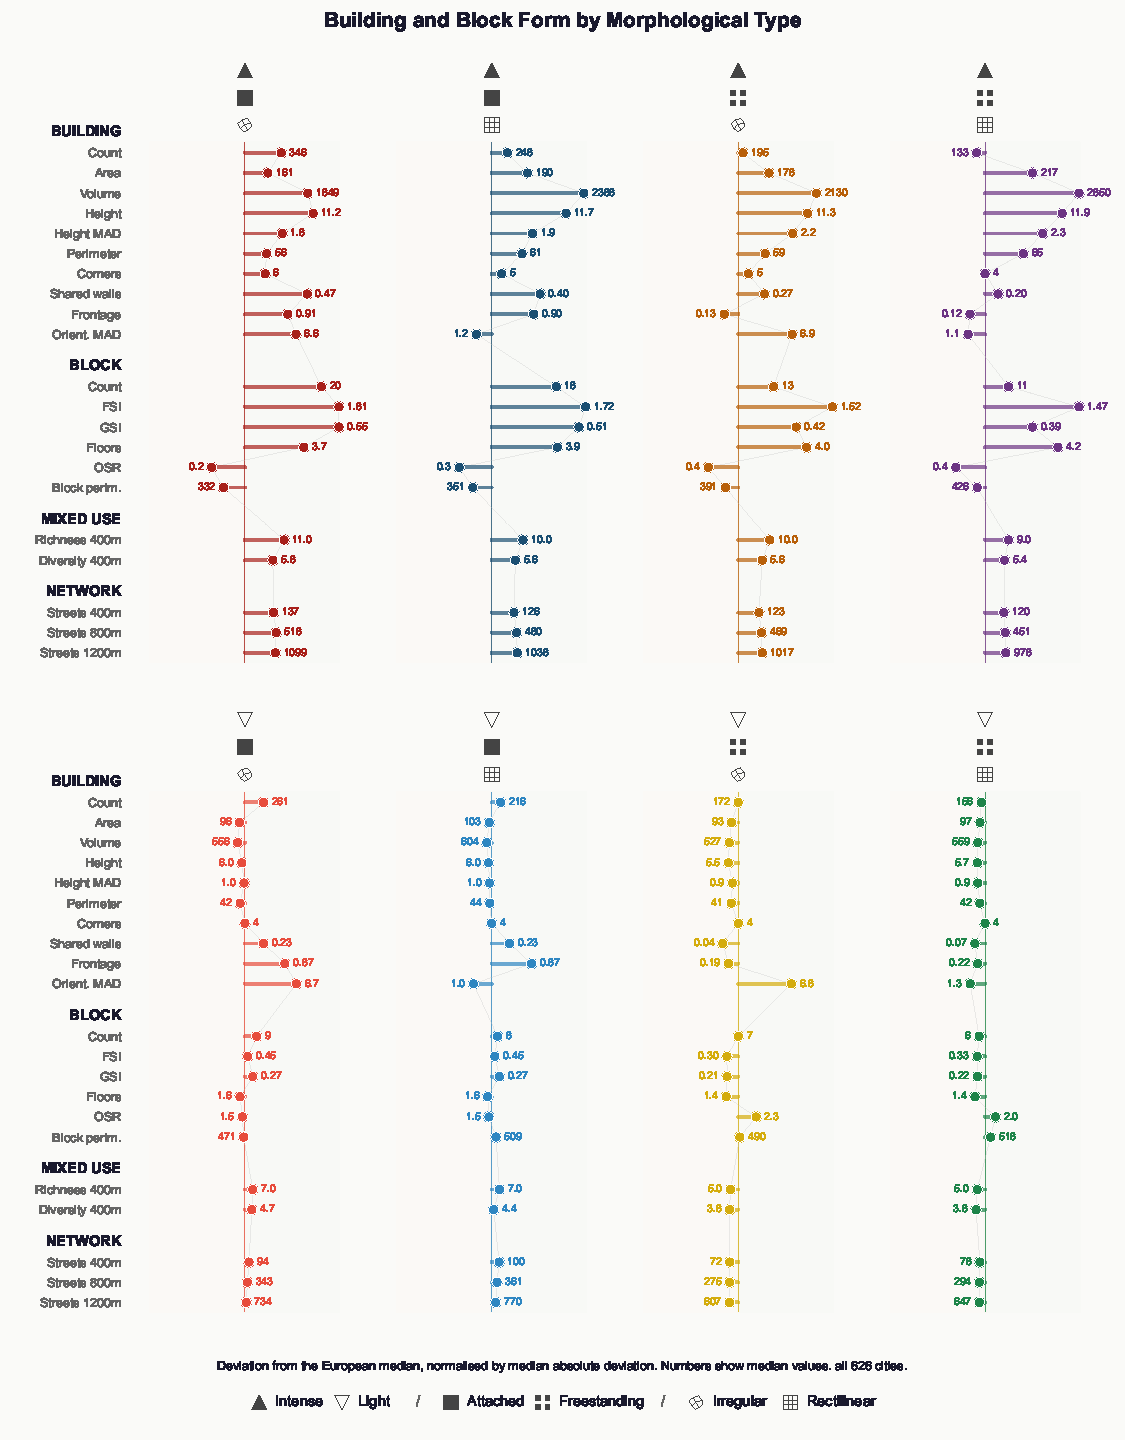
\includegraphics[width=\textwidth]{outputs/atlas/plate4_buildings_full.pdf}
  \caption{As Figure~\ref{fig:plate4}, but using all \nCities{} cities. Deviation profiles are stable; shared wall ratio is the only metric with a material shift, consistent with ML-derived footprint artefacts.}
  \label{fig:plate4_full}
\end{figure}

\section{Continuity axis: notes on measurement and threshold}
\label{sec:continuity-calibration}

Figure~\ref{fig:frontage_validation} validates the frontage ratio as a continuity measure and the 0.75 threshold.

At the city level, median frontage ratio varies from near zero in Finnish and Polish cities, where freestanding apartment blocks and detached houses dominate, to its highest in Greek cities with dense Mediterranean infill (Figure~\ref{fig:frontage_validation}A). The ordering follows known housing traditions: the Netherlands and Belgium (terraced canal and row houses) rank high; Nordic and Central European cities (freestanding blocks, regulated open space) rank low. Romania ranks higher than its eastern European neighbours, consistent with its dense historic urban cores. Italy and Spain span the full range within their borders, reflecting the coexistence of compact historic cores and dispersed suburban development.

Frontage ratio is only modestly correlated with FSI at the city level (Pearson $r = \rFrontageFSIcity$): denser cities tend towards somewhat higher frontage, but the two axes share little variance, so the Continuity axis still captures configuration that Intensity does not. A city can be high-intensity with freestanding towers or low-rise with continuous terraces; frontage distinguishes these configurations where FSI does not.

Splitting streets by intensity reveals distinct distributional shapes (Figure~\ref{fig:frontage_validation}B). Low-intensity streets (FSI $<$ \threshFSI) show a broad interior peak and a declining tail, consistent with the mixture of detached houses, terraces, and low-rise courtyards that make up most European low-intensity fabric. High-intensity streets (FSI $\geq$ \threshFSI) instead ramp monotonically towards a mode at 1, the perimeter-block form characteristic of high-intensity European centres. The two distributions cross near two-thirds: above this value, high-intensity streets outnumber low-intensity streets at every frontage level. The \threshCont\ threshold sits above the crossover, in the range where continuous-frontage fabric dominates both subsets. The choice of \threshCont\ rests on interpretability: a street where at least three-quarters of its more-fronted side is occupied by building facades reads as predominantly enclosed.

\begin{figure}[p]
  \centering
  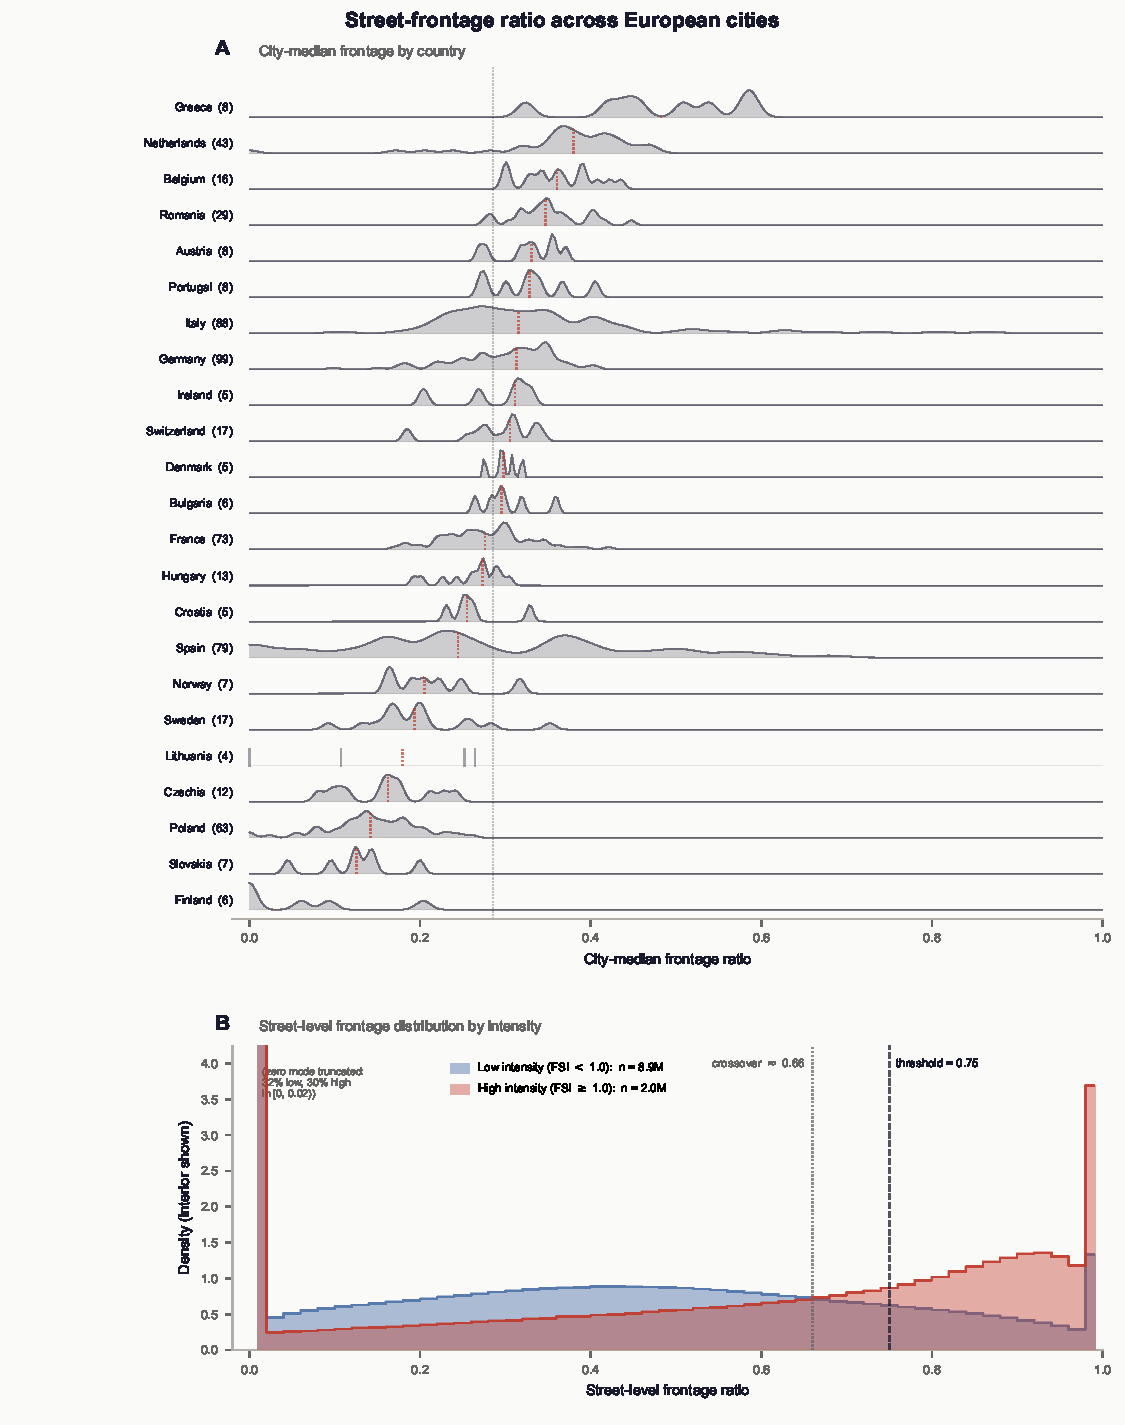
\includegraphics[width=0.92\textwidth]{outputs/atlas/validation/frontage_validation.pdf}
  \caption{Street-frontage ratio across European cities. (A)~Ridgeline densities of city-median frontage ratio by country (kernel density estimates where $n \geq 5$, rug ticks otherwise), ordered by national median (dotted red drop-line); the dotted grey line marks the grand median across all cities. (B)~Street-level frontage distribution split by intensity: density histograms for low-intensity (FSI $<$ \threshFSI, blue) and high-intensity (FSI $\geq$ \threshFSI, red) streets. The dominant zero mode (freestanding facades on both sides of the street) is truncated to show interior structure; the truncated fraction is annotated in-panel. The dashed line marks the \threshCont\ classification threshold; the dotted grey line marks the distribution crossover near two-thirds where high-intensity streets begin to outnumber low-intensity streets.}
  \label{fig:frontage_validation}
\end{figure}

\section{Axis selection and classification validity}
\label{sec:axis-selection}

\emph{Variable choice.} Among four candidate intensity variables, FSI discriminates between types most strongly (mean $\eta^2 = \etaSqCandFsi$, versus \etaSqCandHeight{} for height and \etaSqCandGsiCand{} for ground-space index), because it integrates vertical extent and horizontal coverage in a single measure.

\emph{Axis independence.} The three axes carry largely independent information. Across \nAxesM{} million classified streets, the Pearson correlation between Intensity and Continuity is \rIntCont{}, and correlations involving Irregularity are close to zero (\rIntIrreg{} with Intensity, \rContIrreg{} with Continuity); all eight types are populated.

\emph{External validity.} As a check that the classification captures properties it was not built from, type membership also discriminates fabric variables not used in its construction: it explains \etaSqGsi{} of the variance in ground-space index and \etaSqHeight{} of building height (the $\eta^2$ statistic); building count per walking neighbourhood is only weakly discriminated ($\eta^2$ = \etaSqBldgDensity{}).

\section{Analytical supplement: within-city patterns}
\label{sec:analytical-supplement}

The plates in the main text describe cross-sectional patterns. This appendix looks at the same patterns within cities, using city-demeaned regression models and matched-pair comparisons across \nAnalysisMStreets{} million classified streets in \nAnalysisCities{} urban centres with complete predictor coverage. Models include city-clustered standard errors and 10\% spatial subsampling to reduce overlap from the \kernelDist\,m distance-weighted kernel. The results are broadly consistent with the plate-level observations, though the within-city framing brings some additional texture.

Table~\ref{tab:decomposition} shows within-city $R^2$ for five nested models predicting service distance (log-transformed). The morphological axes together account for a modest but consistent share of within-city variance (\rSqMorphMin--\rSqMorphMax\% for commercial outcomes), and adding street network structure raises this to \rSqMorphNetMin--\rSqMorphNetMax\%. Census-resolution population density adds little once morphology is included, though this comes with a scale caveat: the 1\,km$^2$ grid is coarser than the \kernelDist\,m morphological kernel, and a finer-grained density measure might alter this conclusion.

\begin{table}[ht]
  \centering
  \caption{Within-city $R^2$ by predictor family. All models use city-demeaned
    (within-city) estimation with 10\% spatial subsampling. Population density's
    marginal $\Delta R^2$ when added to the full model is at most 0.026 across outcomes.}
  \label{tab:decomposition}
  \small
  \begin{tabular}{lrrrrrr}
    \toprule
    Model & Retail & Eat \& drink & Education & Health & Green space & Trees \\
    \midrule
    Pop.~density alone & 0.139 & 0.172 & 0.172 & 0.185 & 0.033 & 0.000 \\
    3 morph.~axes alone & 0.171 & 0.198 & 0.147 & 0.172 & 0.102 & 0.023 \\
    Network alone & 0.122 & 0.148 & 0.162 & 0.159 & 0.036 & 0.003 \\
    3 axes + network & 0.228 & 0.267 & 0.239 & 0.256 & 0.124 & 0.030 \\
    Everything & 0.240 & 0.284 & 0.263 & 0.281 & 0.126 & 0.033 \\
    \bottomrule
  \end{tabular}
\end{table}


Table~\ref{tab:marginal} breaks the morphological contribution down by axis. For commercial services, FSI tends to carry the larger share (\mFSIshareMin--\mFSIshareMax\% of the morphological $R^2$) with frontage adding \mContshareMin--\mContshareMax\% independently. For green space the pattern inverts: frontage accounts for \mContGreenShare\% and FSI only \mFSIGreenShare\%. This mirrors the directional difference visible in the plates.

\begin{table}[ht]
  \centering
  \caption{Marginal $\Delta R^2$ of each predictor family and each morphological axis.
    Within-morphology marginals show the unique contribution of each axis
    when added to the other two.}
  \label{tab:marginal}
  \small
  \begin{tabular}{lrrrrrrr}
    \toprule
    Outcome & Full $R^2$ & $\Delta$ Morph & $\Delta$ Pop.~dens & $\Delta$ Network & $\Delta$ FSI & $\Delta$ Frontage & $\Delta$ MAD \\
    \midrule
    Retail & 0.213 & 0.113 & 0.0000 & 0.041 & 0.132 & 0.019 & 0.000 \\
    Eat \& drink & 0.257 & 0.128 & 0.0000 & 0.053 & 0.171 & 0.011 & 0.002 \\
    Education & 0.227 & 0.084 & 0.0000 & 0.073 & 0.124 & 0.012 & 0.001 \\
    Health & 0.241 & 0.104 & 0.0000 & 0.064 & 0.140 & 0.016 & 0.001 \\
    Green space & 0.130 & 0.089 & 0.0000 & 0.024 & 0.010 & 0.081 & 0.002 \\
    Trees & 0.023 & 0.021 & 0.0000 & 0.004 & 0.002 & 0.010 & 0.004 \\
    \bottomrule
  \end{tabular}
\end{table}


Table~\ref{tab:matched} uses coarsened exact matching on city and population-density quintile to compare attached and freestanding streets within the same density band. Streets with attached building fabric tend to be \matchedGainMin--\matchedGainMax\,m closer to commercial services, with the direction consistent across \matchedDirMin--\matchedDirMax\% of cities. For green space the difference runs the other way: attached streets are on average \matchedGreenLoss\,m farther from the nearest green-space polygon.

\begin{table}[ht]
  \centering
  \caption{Within-city matched-pair comparison: Attached vs Freestanding streets,
    matched on city and population-density quintile. Effect is the difference
    in mean distance (Attached minus Freestanding); negative values indicate
    Attached streets are closer. \%~cities shows the proportion of cities
    where the effect is in the indicated direction.}
  \label{tab:matched}
  \small
  \begin{tabular}{lrrrrrr}
    \toprule
    Outcome & Effect (m) & Median & P25 & P75 & \% cities & $N$ cities \\
    \midrule
    Retail & -43.9 & -45.0 & -58.4 & -32.5 & 99.0\% closer & 592 \\
    Eat \& drink & -44.9 & -44.6 & -63.2 & -31.1 & 97.3\% closer & 592 \\
    Education & -42.8 & -43.7 & -62.1 & -28.4 & 97.5\% closer & 592 \\
    Health & -43.9 & -43.4 & -60.6 & -29.9 & 97.5\% closer & 592 \\
    Green space & +36.8 & +35.7 & +24.7 & +45.2 & 97.8\% farther & 592 \\
    Trees & +17.7 & +15.1 & +10.2 & +21.2 & 96.8\% farther & 592 \\
    \bottomrule
  \end{tabular}
\end{table}


The same within-city lens clarifies which demographic gradients are morphological and which reflect between-city composition. Population density is the clearest separator: every Intense type exceeds every Light type with no overlap (Plate~8). Among the compositional shares (Table~\ref{tab:demo-robust}), the child and working-age gradients persist once cities are demeaned and hold in a clear majority of cities; the apparent employment gradient, by contrast, is a between-city effect (its pooled Light--Intense gap collapses under city-demeaning and its direction holds in only about half of cities), while the elderly share is flat throughout. The main text therefore reports the child and working-age gradients but not employment.

\begin{table}[ht]
  \centering
  \caption{Within-city robustness of demographic gradients, Light versus Intense types. The pooled gap is the Light$-$Intense difference in median share (percentage points). The city-demeaned effect (Cliff's $\delta$) removes between-city differences, so values near zero indicate no within-city signal. The final column is the share of cities (with $\geq$30 streets in each group) whose within-city direction matches the pooled sign.}
  \label{tab:demo-robust}
  \small
  \begin{tabular}{lrrr}
    \toprule
    Demographic & Pooled gap (pp) & City-demeaned $\delta$ & Cities consistent (\%) \\
    \midrule
    Children ($<$15)     & $\demoChildGap$ & $\demoChildDelta$ & \demoChildPct \\
    Working age (15--64) & $\demoWorkGap$  & $\demoWorkDelta$  & \demoWorkPct \\
    Elderly ($\geq$65)   & $\demoElderGap$ & $\demoElderDelta$ & \demoElderPct \\
    Employment           & $\demoEmpGap$   & $\demoEmpDelta$   & \demoEmpPct \\
    \bottomrule
  \end{tabular}
\end{table}

\end{document}
